\documentclass[preprint,12pt]{elsarticle}

\journal{Computers \& Operations Research}

\usepackage{latexsym} \usepackage{subcaption} \usepackage{graphicx}
\usepackage{mathptmx} \usepackage{placeins}
%
%****************************************************************************
%AUTHOR: You may want to use some of these packages. (Optional)
\usepackage{amsmath} \usepackage{amsfonts} \usepackage{amssymb}
\usepackage{amsbsy} \usepackage{amsthm} \usepackage{booktabs}
\usepackage{epsfig}

\usepackage{caption} \usepackage{standalone} \usepackage{tikz}
\usetikzlibrary{arrows} \usetikzlibrary{decorations.markings}
\usetikzlibrary{calc} \usetikzlibrary{shapes}

\usepackage{natbib}
% \usepackage{authblk}

%****************************************************************************


%
%****************************************************************************
%AUTHOR: If you do not wish to use hyperlinks, then just comment out the
%hyperref usepackage commands below.

%% This version of the command is used if you use pdflatex. In this case you
%% cannot use ps or eps files for graphics, but pdf, jpeg, png etc are fine.

\usepackage[colorlinks=true,urlcolor=blue,citecolor=black,anchorcolor=black,linkcolor=black]{hyperref}

%% The next versions of the hyperref command are used if you adopt the
%% outdated latex-dvips-ps2pdf route in generating your pdf file. In
%% this case you can use ps or eps files for graphics, but not pdf, jpeg, png etc.
%% However, the final pdf file should embed all fonts required which means that you have to use file
%% formats which can embed fonts. Please note that the final PDF file will not be generated on your computer!


%%\usepackage[dvips,colorlinks=true,urlcolor=blue,citecolor=black,%
%% anchorcolor=black,linkcolor=black]{hyperref}
%****************************************************************************


%
%**************************************************************************** *
%* AUTHOR: YOUR CALL!  Document-specific macros can come here.  *
%****************************************************************************
%Packages added manually
\usepackage{xcolor} \usepackage{multirow} \usepackage{pdflscape}
\usepackage{comment}

%######################################################### * *  The Document.  *
\begin{document}

\begin{frontmatter}


\title{Evaluating Heterogeneous Ambulance Fleet Allocations in Jakarta}

\author[inst1]{Geraint Palmer} \author[inst1]{Mark Tuson} \author[inst1]{Sarie
    Brice} \author[inst1]{Paul Harper} \author[inst1]{Vincent Knight}
    \author[inst2]{Leanne Smith} \author[inst1,inst3]{Daniel Gartner}


\affiliation[inst1]{organization={School of Mathematics, Cardiff
    University},%Department and Organization addressline={Abacws, Senghennydd
    Road}, city={Cardiff}, postcode={CF24 4AG}, state={Wales}, country={United
    Kingdom}}
            
\affiliation[inst2]{organization={Welsh Ambulance Services NHS
    Trust},%Department and Organization addressline={Beacon House, William Brown
    Close}, city={Cwmbran}, postcode={NP44 3AB}, state={Wales}, country={United
    Kingdom}}

\affiliation[inst3]{organization={Aneurin Bevan University Health
    Board},%Department and Organization addressline={Lodge Road},
    city={Caerleon}, postcode={NP18 3XQ}, state={Wales}, country={United
    Kingdom}}

%% Text of abstract  100-200 words

%A self-contained abstract of about 100-200 words outlining the aims, scope and
    %conclusions of the paper must be supplied..
 \begin{abstract} Ambulance services have a duty of care to the clinical
     outcomes of the population they serve, and therefore aim to maximise the
     chances of survival and improve patient outcomes following a medical
     emergency. Despite this, although the ambulance location-allocation problem
     has been widely studied, it has predominantly focused on minimising
     response times or maximising coverage alone, and not explicitly for
     considering patient outcomes. In this paper we propose a modelling approach
     to consider where to optimally locate different types of emergency response
     vehicles in order to maximise patient outcomes within a heterogeneous
     population.  To achieve this, we develop a heuristic algorithm for finding
     better fleet allocations which is used in conjunction with a discrete-event
     simulation model of ambulance services with heterogeneous vehicles. Our
     approach is informed by, and tested on, real-world data from Jakarta,
     Indonesia. Using our developed models, decision makers are better able to
     understand ambulance fleet capacity needs and locations, and their impact
     on patient outcomes.

\end{abstract}


%%Research highlights
% Please use 'Highlights' in the file name and include 3 to 5 bullet points
% (maximum 85 characters, including spaces, per bullet point).
\begin{highlights} \item A sequential simulation for ambulance demand and
    capacity planning \item Mathematical modelling for maximising survival with
    heterogeneous patients and fleets \item Cross-entropy heuristic algorithm
        for finding better fleet allocations \item Application to Jakarta for
            policy recommendations and testing future demand scenarios
% \item Output evaluation using several performance metrics and levels of detail
            % %72 characters incl. spaces \item Our approach determines the
            % trade-off between different allocation levels and transportation
            % modes \item Comparisons with real-world ambulance data reveal the
            % potential of allocation strategies
\end{highlights}

\begin{keyword}
% maximum of six keywords
%% keywords here, in the form: keyword \sep keyword
Ambulance Planning \sep Emergency Medical Services \sep Simulation \sep Health
Care \sep Optimisation \sep Mathematical Modelling \end{keyword}

\end{frontmatter}


\newpage

%%\tableofcontents

\section{Introduction and Background}

%% This sentence needs to be in the beginning because it sets the focus on "life saving" or "life threatening"
Time-critical conditions (TCCs) are a substantial cause of mortality worldwide,
responsible for an estimated 54\% of all deaths \cite{FraserBMJ}. Emergency
medical services (EMS) play a pivotal role in responding to TCCs and saving
patients from life-threatening medical conditions. Most EMS research, especially
planning to meet increasing ambulance demands, tends to be focussed on
high-income countries including, for example, Australia
\cite{lowthian2011increasing}, Germany \cite{veser2015demographic}, and USA
\cite{birmingham2021trends}. In contrast, most low and middle-income countries
(LMICs) lack an organised EMS system, with most ambulances used purely for
patient transport and not as an emergency care vehicle \cite{plummer2017ems}.
However, the burden of deaths due to TCCs is much greater in LMICs than in
high-income countries, the difference being around threefold \cite{ChangPMC}.
For traffic accidents, strokes and heart attacks, rapid access to appropriate
treatment is especially vital. 

The application of our research is focused on Indonesia, as supported by an
award for Global Challenges Research Funds (GCRF). In Indonesia, an LMIC, there
has been very little prior work on developing an EMS strategy, driven largely by
inadequate resources including a lack of financial investment and human capital
\cite{plummer2017ems,pusponegoro2003terrorism,yusvirazi2018state}. Related
research by the authors \cite{BriceSyaribahNoor2022Esui} has highlighted
particular challenges in Indonesia as a lack of a single coordinated EMS, the
ability or willingness to pay for an ambulance, a large geographical area, and
areas of severe traffic congestion especially in Jakarta, the capital.  

When our research programme commenced in October 2019, ambulance services in
Jakarta were provided by many disparate, mostly private providers that charge
patients for their use, such as private hospitals. We initially partnered with
Ambulans 118, a non-government charitable ambulance service established in 2005
by the Indonesian Surgeons’ Association, that  currently operates in five cities
across Indonesia: Jakarta, Palembang, Yogyakarta, Surabaya and Makasser. Unlike
private providers, Ambulans 118 suggests that a donation is made for use of its
EMS vehicles, but otherwise provides free emergency medical care and is also
leading on paramedic training across the country. 

The overarching goal of our research was to work with the Indonesian Government,
the different ambulance providers, and hospitals, to help them forecast
emergency demand and make critical decisions on the optimal types, capacities
and geographical locations of emergency vehicles within a potentially
co-ordinated EMS system, starting with Jakarta. To facilitate this, in
collaboration with Ambulans 118 we organised workshops in Jakarta in February
2020, thankfully just before the COVID-19 pandemic and lockdowns, which were
attended by over 170 people including doctors, nurses, paramedics, academics,
and officials from the Indonesian Ministry of Health. This paper presents some
aspects of the overall research programme, specifically focusing on the
development of a simulation model and location-allocation heuristics for
maximising patient survival.  

Fundamental to the project and the research described in this paper was an
initial study that we carried out in order to better understand patient needs
and the barriers to use of ambulances in Indonesia. Throughout the month of
December 2020, we undertook comprehensive surveys in Emergency Departments (EDs)
across Jakarta and published the first known study in to EMS demand within the
country \cite{BriceSyaribahNoor2022Esui}. Our study showed that the utilisation
of ambulances by patients attending EDs is considerably low and of concern. The
low utilisation is contributed to patients’ lack of awareness of available
ambulance services given a lack of coordination, patients’ disinclination to use
ambulances due to high costs, and long response times.  All of these barriers
impact on patient outcomes, especially for those with  life-threatening
conditions. For example, remarkably more trauma patients took a car-share ride
(20\%) or motorcycle (20\%) to reach the ED than an ambulance (just 10\%), while
only 14\% of critical cardiovascular patients used an ambulance compared to 67\%
travelling to hospital by private car or a car-share ride.

The first contribution of this paper is the development of a comprehensive
sequential discrete event EMS simulation that models and evaluates heterogeneous
fleet allocations of emergency vehicles by utilising a novel approach in which
transit jobs, rather than patients, are framed as the queueing `customers'. Our
methodology utilises two discrete event simulations of the same system that are
run sequentially and together combine to form the logic of a single simulation
of a heterogeneous fleet; and key performance indicators (KPIs) are calculated
by making use of survival functions. Secondly, we extend the work of
\cite{Knight2012918} to consider both heterogeneous patients and heterogeneous
fleets, utilising a cross-entropy heuristic to find allocations that maximise
patient survival. The resulting allocations are evaluated using the discrete
event simulation. Thirdly, we demonstrate the use and impact of our modelling
framework applied to current and proposed ambulance allocations in the city of
Jakarta, thus supporting Government-level decision making with an overall goal
to improve the lives of those living in LMICs.  This leads to decision support
and managerial insights in Indonesia, although the developed modelling framework
could be readily applied to other locations.

The paper is structured as follows: Section~\ref{sec:litreview} gives an
overview of the literature on modelling ambulance allocations.
Section~\ref{sec:simulation} outlines the logic of the sequential discrete event
simulation models for heterogeneous fleets. Section~\ref{sec:jakarta} describes
the current emergency service situation in Jakarta and presents simulation
results from current and proposed fleet allocations.
Section~\ref{sec:betterallocations} describes the survival objective and
heuristic algorithm to find better fleet allocations, and
Section~\ref{sec:discussion} discusses the findings and contributions of the
paper.

\section{Literature Review}\label{sec:litreview}

There is a rich literature on Operational Research applied to EMS location and
related allocation problems. Literature reviews that include these topics are
\citet{aringhieri2017emergency, belanger2019recent, farahani2019or, Li2011,
Liu2021, reuter2017logistics} and  \citet{wang2021emergency}.

Emergency medical services can be evaluated using different performance measures
with coverage and response time being the predominant metrics
\cite{Mclay2010evaluating}. However, missing a response time target by just one
second, for example, would be considered as a `failure' in many models with no
appreciation at all of the impact on patient survival or outcome
\cite{Mclay2010evaluating}. This seems somewhat restrictive and short-sighted,
which is why we focus on survival as a metric and thus, in the following,
compare and contrast papers using that metric with our approach.

Table \ref{tab:RelatedWork} provides an overview of recent research that focus
on the survival metric. We break down related papers into discrete-event
simulation~(DES), queueing theory and optimisation methods, and we provide a
summary of each paper from the table as well as compare and contrast them with
our modelling and solution approach.

\begin{table}[htbp] \centering \small \resizebox{\textwidth}{!}{%
        \begin{tabular}{llcccc} \toprule Reference   & Year & DES & Queueing
            Theory & Optimisation \\ \midrule \citet{amorim2019integrated} &
            2019 &  & & \checkmark \\ \citet{boutilier2022drone} & 2022 &  &
            \checkmark \\ \citet{Erkut200842} & 2008 & & & \checkmark\\
        \citet{Knight2012918} & 2012 & & \checkmark & \checkmark \\
        \citet{MCormack2015} & 2015 & \checkmark & & \checkmark\\ \bottomrule
        \end{tabular}% } \caption{Break down of related research that focuses on
        survival.\label{tab:RelatedWork}} \end{table}

\FloatBarrier


 % The original work considered average response time optimisation models,
% whereby emergency vehicles are allocated such that travel time is minimised.
% However these typically:
%\begin{itemize} \item fail to capture the extent of variation in the data and
%may provide an unequitable solution for the population; \item are not as
%sensitive to dispatch rules compared with travel time distribution based models
%\textbf{(Chelst 1979)}, so are more beneficial for strategic policy
%investigations, but less so for tactical and operational modelling; \item are
%misaligned with modern day emergency services, whereby, average response time
%is not a measure of significance, instead the focus is on system wide service
%delivery.  \end{itemize}

%The table reveals that coverage in terms of a population is a widely used
%measure as a proxy for patient survival in EMS location-allocation planning.
%More specifically,

\citet{amorim2019integrated} propose an integrated strategic and tactical
planning approach which features an optimization model and a local search
heuristic based on Gaussian Processes.  Their methodology is applied to the city
of Porto while reporting on performance metrics such as survival. Our approach
is different because we use a discrete-event simulation framework and a
cross-entropy optimisation approach to determine the number of ambulances
required in each station. 


\citet{boutilier2022drone} develop an integrated location-queueing model that
incorporates existing EMS response times in a drone network. They use a p-median
approach and an Erlang loss model. Although survival is not their main
optimization criterion,  they report how many patients would survive using their
approach.

Erkut et al.~\cite{Erkut200842} can be considered the first modelling approach
that considers decaying survival probabilities during response time.  The
rationale is, because survival can be thought of as a more robust and generic
objective for EMS performance measurement than coverage or average response
time. In an application of a recently developed Maximal Survival Location
Problem model (MSLP), the authors use data from Edmonton, Canada and  show that
maximising survival is superior to other objectives in clinical outcome for
cardiac arrest patients.

McCormack and Coates~(2015)~\cite{MCormack2015} focus on the optimization of EMS
vehicle fleet allocation and base station location through the use of a genetic
algorithm (GA) with an integrated EMS simulation model. Their objective is
maximization of the overall expected survival probability across patient
classes. Applications of the model were undertaken using real call data from the
London Ambulance Service. The difference between their modelling approach and
our is that we have a different survival function, focus on a different
heuristic optimization and evaluate our approach with data from a development
country and have higher traffic volume and congestion in our data. 

Knight, Harper and Smith \cite{Knight2012918} provide a supporting extension of
the MSLP that allows it to be applied more generally to real-world EMS systems,
acknowledging that different patients have varying levels of expected survival
probabilities.  The Maximum Expected Survival Location Model for Heterogeneous
Patients, MESLMHP, allows multiple classes of patient groups to be defined,
where previously only cardiac arrest patients formed part of the objectives for
primary response.  In reality, by definition any emergency patient has a
necessity for swift attendance, and a timely response to any incident type may
impact on clinical outcome in some way. It is for this reason MESLMHP is
designed to be generic enough to accommodate any number of patient groups, with
each class weighted dependent upon the relative urgency of the incident.  More
than just a contribution to the model’s demand input, these patients are
included in the optimisation when maximising total population survival
probability.

%Two tiers to the EMS model realized the different demands on two vehicle
%classes; ambulances and rapid response cars. Multiple patient classes were
%modelled and survival functions used to differentiate the required levels of
%service.  The simulation model was shown to effectively emulate real-life
%performance. Optimization of the existing resource plan resulted in significant
%improvements in survival probability. Optimizing a selection of 1 hour periods
%in the plan, without introducing additional resources, resulted in a notable
%increase in the number of cardiac arrest patients surviving per year. The
%introduction of an additional base station further improved survival when its
%location and resourcing were optimized for key periods of service. Also, the
%removal of a base station from the system was found to have minimal impact on
%survival probability when the selected station and resourcing were optimized
%simultaneously.

%\begin{itemize} \item Money and lives saved is a more coherent message for
%health service public forums and reassure that the service is putting the
%patient at the heart of their operations; \item Survival is already a key
%message in many public health and emergency campaigns, with stroke and heart
%attack campaigns featuring heavily in the media in recent years; \item EMS
%targets may differ around the world, but maximising patient survival is a
%common objective; \item Coverage is a proxy for survival – explicitly using
%survival simply streamlines the objective; \item Evidence from previous studies
%shows preferable patient outcome with survival based allocation objectives.
%\end{itemize}


%Pan et al.~\cite{ShengliPan201234} focus on binary coverage using mathematical
%programming. In contrast, our work considers a patient-centric metric. Another
%major difference is that we propose a probabilistic model and solve use
%simulation modelling paired with a heuristic algorithm to find fleet
%allocations.




%while \cite{Berman2003474} focus on gradual coverage. \cite{Revelle1988143}
%use a reliability measure to account for variance in resource availability.

%This concept links to the idea of response performance since coverage is
%measured by travel time or distance between the EMS vehicle station (or standby
%points) and patient locations; however, it is also subject to two types of
%errors (pointed out in \cite{Erkut200842}) and one solution limitation:
%\begin{itemize} \item Measurement Error – a lack of distinction between covered
%and uncovered areas, and results within a covered area; \item Optimality Error
%– inequitable resource distribution for a population; \item Threshold
%Limitation – theoretical capped improvement, where in reality, the system has
%continuous improvement gains given more resources.  \end{itemize}

%After years of response based EMS performance modelling, research is gradually
%moving towards more clinical outcome based measures, whereby survival and
%post-treatment quality of life of patients are starting to be considered.
%Although the quantity of survival-maximising literature is still small in
%comparison to response target led approaches, it is supported by a
%strengthening focus in this by ambulance services themselves.  For example in
%the UK, like in many developed nations, encouragement for innovative and
%patient-centred approaches stems in general from a pressure of ageing and
%sicker populations, increasing demand \textbf{(National Audit Office 2011)}, a
%shift in activity to lower acuity, and the need for healthcare reform (House of
%Commons 2011; NHS 2014).  



  

% \section{Quantifying Allocation Effectiveness: MESLMHPHF Score}

% \subsection{MESLMHPHF Score} %% TODO: VK We build on previous work by the
% authors \cite{Knight2012918} who developed the Maximal Expected Survival
% Location Model for Heterogeneous Patients, MESLMHP. It is helpful here to
% briefly revisit the MESLMHP model as a point of reference for the extension
% (Section 4) and for ease of comparison in the case study (Section 5). 

% \subsection{MESLMHP formulation} Let $m$ denote the number of demand nodes,
% $n$ the number of service nodes and $k$ the number of patient types.  Using
% the notation $[a]=\{x \; | \; 1 \leq x \leq a\}$ for any $a \in Z$, where
% $m,n,k \in Z$, let the demand of type $l \in [k]$ from demand node $i \in [m]$
% be denoted by $\lambda_i^l$.  The average ambulance utilisation at a given
% service station $j \in [n]$ is given by $\pi_j$ and the probability that a
% vehicle at station $j$ is available to respond is therefore $(1-\pi_j )$.  

% To maintain an order of preference for all stations in allocation to each
% demand node, let $\rho \in R_{\geq0}^{(m\ast n)}$ denote the preference
% matrix; for demand node $i$, the $j^{th}$ favoured choice of station,
% $\rho_{ij}$, having no available vehicle (occurring with probability$
% \pi_{\rho_{ij}}^{x_j}$, where $x_j$ is the number of vehicles located at the
% station $j$) implies the $(\rho_{i,j+1})^{th}$ service node will be the next
% station to be selected.  

% It is possible to have a different survival function for each patient type $l,
% s_l: \mathbb{R}_{\geq 0} \Rightarrow [0,1]$.  For each demand-service node
% pair, the travel time is required as input to the model, represented by travel
% matrix $t_{i,j} \in \mathbb{R}_{\geq 0}^{m \ast n}$.  Finally, since the
% different groups of patients are based on the urgency of the medical
% condition, a weight $w_l$ for each patient type is required in order to
% prioritise the demand.

% Commencing with the probability of survival of a patient of type $l$ from
% demand node $i$, serviced by station $\rho_{ij}$, the formulation is as
% follows: \begin{equation} P_{i,\rho_{ij}}^l = s_l \left(t_{i,\rho_{ij}}\right)
% \left(1-\pi_{\rho_{ij}}^{x_{\rho_{ij}}}\right)
% \prod_{r=1}^{j-1}\pi_{\rho_{ir}}^{x_{\rho_{ir}}} \end{equation}

% Therefore, the objective of MESLMHP is to maximise the weighted sum over
% demand nodes for each of the patient groups, $f(z)$ (with specific capacity
% $z$), where

% \begin{equation} f(z) =
% \sum_{l=1}^{k}w_l\sum_{i=1}^{m}\lambda_i^l\sum_{j=1}^{n}P_{i,\rho_{ij}}^l
% =\sum_{l=1}^{k}w_l\sum_{i=1}^{m}\lambda_i^l\sum_{j=1}^{n}s_l \left(t_{i,
% \rho_{ij}}\right) \left(1-\pi_{\rho_{ij}}^{x_{\rho_{ij}}}\right)
% \prod_{r=1}^{j-1}\pi_{\rho_{ir}}^{x_{\rho_{ir}}} \end{equation}

% such that \begin{equation} \sum_{j=1}^n x_j = z \;\;  \text{and} \;\;  x_j \in
% \mathbb{Z}_{\geq 0} \end{equation}




% \subsection{Survival Calculation}

% In reality, some emergency incidents do not result in a substantive
% deterioration of a patient’s status over time; however, in all situations,
% there is a reasonable cut-off beyond which a patient should not expect to have
% to wait for care.  In the UK for example, this varies from twenty minutes to
% four hours, dependent upon the criticality.  Consequently, a mixture of
% theoretical survival functions and step functions can be utilised by the
% single allocation optimisation model (equation 2), representing the different
% objectives (clinical or time focused), as well as the varying levels of
% patient criticality, and the effect of response management upon the
% population’s health. 

% Survival probabilities for critical incidents, calculated from a theoretical
% monotonically decaying survival function reported in the literature
% \cite{Valenzuela20001206} are used to demonstrate an attainable level of
% success from a response.  The survival curve $s(t)$ (equation 4) selected for
% this study is shown in Figure 1 alongside a step or hard-target function
% (equation 5) representing an example of a typical EMS response time target in
% minutes.  The survival curve, $s(t)$, represents survival until hospital
% discharge following cardiac arrest; its origins are explained in detail by
% Knight, Harper and Smith \cite{Knight2012918}.

% \begin{equation} s(t) = \left(1 + e^{0.26+0.139t}\right)^{-1} \end{equation}

% \begin{equation} h(t) = \begin{cases} 1 \text{ if } 0\leq t \leq 8 \\ 0 \text{
% if } t > 8 \end{cases} \end{equation}

% \begin{figure}[ht] \centering
% 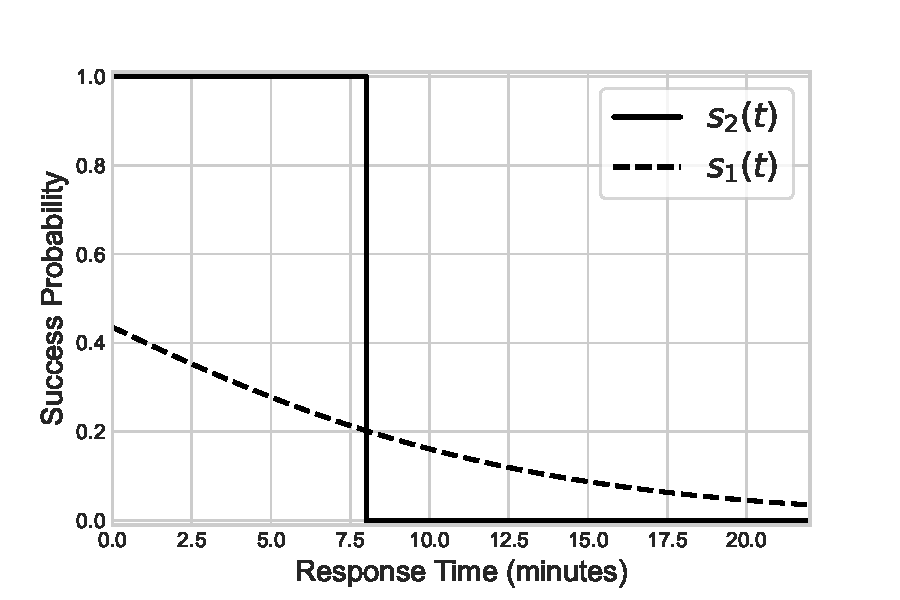
\includegraphics[width=0.6\textwidth]{img/Survival_Function_(new).pdf}
% \caption{Survival function $s(t)$, estimated by Valenzuela et al.
% \cite{Valenzuela20001206} compared with a current EMS target, $h(t)$,
% represented as a step function (binary coverage).}
% \label{Figures:survivalfunction} \end{figure} \begin{comment} Check Figure it
% seems inaccurate \end{comment}

% When system performance using the hard target approach is translated into
% survival, the current 8 minute UK response target greatly overestimates
% clinical outcome for the most critical patients responded to within 8 minutes,
% yet predicts no positive outcome whatsoever for patients responded to after
% this cut-off.  The survival curve $s(t)$ offers a more realistic view of the
% chance of success following a response for more than just cardiac arrest
% patient groups. 

% \subsection{MESLMHPHF constructs} \label{sec:MESLMHPHF} The model described in
% Section 3.1, advances the MSLP by considering different classes of patients;
% however to enhance its realism further, multiple vehicle types are now
% incorporated.  By enhancing the formulation of the MESLMHP, to accommodate a
% fleet that is both heterogeneous in type and purpose, the MESLMHPHF is
% generated.  This new model is formulated in the following sections of this
% paper, and is evaluated in terms of an improved allocation of multiple
% ambulance resources in order to maximise survival of a heterogeneous
% population.   A typical EMS fleet in many countries, including the UK, is made
% up of two main types of vehicle – Emergency Ambulances, EAs (slow but capable
% of conveyance; that is they can transfer the patient to hospital), and Rapid
% Response Vehicles, RRVs (which respond quickly but cannot convey).  Previous
% models, that assume only a homogeneous fleet, ignore the full nature of
% ambulance service delivery, whereby certain combinations of vehicles and crews
% must be dispatched to each particular type of incident.  We now address
% directly the aspiration to serve the highly varying types of medical
% emergencies with the most appropriate sub-fleet resource. 


% The logic of the service extension from a homogeneous fleet (MESLMHP) to two
% vehicle types or sub-fleets is now described, allowing the formulation of the
% Maximal Expected Survival Location Model for Heterogeneous Patients and
% Heterogeneous Fleet, MESLMHPHF.\\ Consider two different sets of patient
% groups, defined as: \begin{itemize} \item $k_1$: Highly critical patients
% (such as cardiac arrest, heart attack or stroke patients) to be responded to
% by either: \begin{itemize} \item 	the most preferable (closest) RRV initially
% for immediate paramedic attention, and to be followed up by the most
% preferable (closest) EA response for conveyance when available – assumes the
% RRV can reach the scene faster than the chosen EA; \item or by the most
% preferable (closest) EA only – assumes no RRVs available, or the most
% preferable RRV cannot reach the scene faster than the most appropriate EA;
% \end{itemize}	\item $k_2$: Less critical patients that require only EA
% attendance.  That is, RRV responses are not considered in this dispatch
% decision.  \end{itemize} (That is, RRV attendance to $k_1$ patients is
% dependent on RRV availability and the speed of response of EA vehicles.)\\


% Such a mixed responder service, as is common throughout the world, means that
% multiple response options are available to dispatchers, enabling the
% organisations to deliver the most appropriate care to each patient.  For two
% patient sets, served by a two sub-fleet system, these response options can be
% thought to follow one of four mathematical constructs:


% \subsubsection{Construct 1: RRV Responder; k1 Patient} Assume the vehicle type
% $u = 0$ if an RRV, and $u = 1$ if an EA. Let $x_{ju}$ be the number of
% vehicles at station $j$ of type $u$ and $\pi_{j,u}$ the utilisation of these
% vehicles.
    
% For a $k_1$  incident, the elements required for computation of an RRV
% response are the probability of an available RRV at station $j$, busy
% probabilities of all preferred RRVs, and busy probabilities of preferred EAs
% \textit{if and only if} the EAs could have responded more quickly than the
% current RRV. 

% Let $R$ be a variable that indicates whether an EA at a more preferable
% station could reach the scene faster than an RRV at the considered station,
% \begin{equation} R = \begin{cases} 1 \text{ if } (t_{i, \rho_{ir},1} - t_{i,
% \rho_{ij},0}) \leq 0 \\ 0 \text{ otherwise }  \end{cases} \end{equation}
% where, $t_{i, \rho_{ir},u}$ is the travel time of a vehicle of type $u$
% between demand node $i$ and preferred station $\rho_{i,r}$ ($r$ is a greater
% preference than $j$).  If the travel times are equal, the best decision would
% be to dispatch the EA at the preferred station, so for an RRV at $j$ to
% respond, the busy probability of the EA at $r$ is still required in the
% calculation.  The variable $R$ takes a value of 1 if the EA at the more
% preferable station $r$, has a journey time to the scene shorter than (or
% equivalent to) the RRV at the current station$ j$, and a value of 0 if the EA
% would be slower than the current RRV.

% Multiplying these busy probabilities for all stations favoured over station
% $j$, the total probability of only more preferable vehicles being busy is:
% \begin{equation}
% \prod_{r=1}^{j-1}\pi_{\rho_{ir},0}^{x_{\rho_{ir,}0}}\left(\pi_{\rho_{ir},1}^{x_{\rho_{ir},1}}\right)^R
% \end{equation} ($R=0$ creates an EA busy probability of 1 for the preferred
% station, implying that the EA at $r$ would never serve demand of type $l$ from
% node $i$ over an RRV at station  $j$).

% \subsubsection{Construct 2: EA Responder; k1 Patient} For a $k_1$  incident,
% the elements required for computation of an EA response are the probability of
% an available EA at station $j$, busy probabilities of all favoured RRVs and
% EAs, and busy probabilities of less preferred RRVs if and only if the less
% preferable RRVs could have responded more quickly than the current EA.  Let
% $Q$ be a variable that indicates whether an RRV at a less preferable station
% could reach the scene faster than an EA at the considered station,

% \begin{equation} Q = \begin{cases} 1 \text{ if } (t_{i, \rho_{iq},0} - t_{i,
% \rho_{ij},1}) < 0 \\ 0 \text{ otherwise }  \end{cases} \end{equation}

% where $t_{i, \rho_{iq},0}$ is the travel time of a vehicle of type $u$ between
% demand node $i$ and preferred station $\rho_{iq}$ ($q$ is a lower preference
% than $j$).  If the travel times are equal, the best decision would be to
% dispatch the EA at the current station, so the busy probability of an RRV at
% $q$ is not required.  The variable $Q$ takes a value of 1 if the RRV at a less
% preferable station $q$, has a journey time to the scene shorter than the EA at
% the current station $j$.  It takes a value of 0 if the EA would be the quicker
% vehicle to respond.

% Multiplying these busy probabilities over all stations (other than current
% station $j$), the total probability of only more preferable vehicles being
% busy can be written as:  \begin{equation}
% \prod_{r=1}^{j-1}\pi_{\rho_{ir},0}^{x_{\rho_{ir,}0}}\pi_{\rho_{ir},1}^{x_{\rho_{ir},1}}
% \prod_{q=j+1}^{n}\left(\pi_{\rho_{iq},0}^{x_{\rho_{iq,}0}}\right)^Q
% \end{equation}

% ($Q=0$ creates an RRV busy probability of 1 for the less preferable station
% $q$, implying the RRV at $q$ would never serve demand of type $l$ over an EA
% at station $j$).

% \subsubsection{Construct 3: RRV or EA Responder; k1 Patient} Merging the two
% mathematical formulations of constructs 1 and 2, we reach the situation, where
% the probability of either an RRV or an EA being the first responder to an
% emergency of type $k_1$  is calculated.

% The total busy probability for this construct must consider the probabilities
% that all preferable vehicles are busy given a vehicle of type $u$ responds to
% the incident.  \begin{equation}
% \prod_{r=1}^{j-1}\pi_{\rho_{ir},0}^{x_{\rho_{ir},0}}
% \left(\pi_{\rho_{ir},1}^{x_{\rho_{ir},1}}\right)^{\left(R^{1-u}\right)}
% \prod_{q=j+1}^{n}\left(\pi_{\rho_{iq},0}^{x_{\rho_{iq,}0}}\right)^{Q\cdot u}
% \end{equation} To demonstrate that this formulation works as a combined
% construct for any responder type to a $k_1$ patient, consider the following
% examples: For an RRV to have responded from station $\rho_{ij}$, all RRVs at
% preferable stations must be unavailable, and any EAs at preferable stations
% must be unavailable or unable to respond faster.  An RRV response, $u=0$,
% implies the second factor (EA utilisation at station $r$) in the first product
% term of Equation 8, will simplify to be to the power $R$; whereas the power $Q
% \cdot u$ of the utilisation factor (of an EA at station $q$) in the second
% product term reduces to 0, giving the total product value of 1.  Therefore,
% the final form of Equation 8 for an RRV response is equivalent to that of
% Equation 6.

% For an EA to have responded first, all RRVs (that could reach the scene faster
% from preferable or less preferable stations) must be unavailable, and all EAs
% at more preferable stations must be unavailable.  An EA response, $u=1$,
% implies in the first product term in Equation 8, the power of the second
% factor (EA utilisation at $r$) is $R^0=1$; for the second product term, the
% power is simply $Q$, resulting in the formulation given by Equation 7 as
% required.

% \subsubsection{Construct 4: EA Only Responder; k2 Patient } When the demand is
% for an incident type captured by set $k_2$, that is, only an EA is required to
% attend the scene, the total busy probability of all more preferable vehicles
% is the same as given in the MESLMHP formulation of Equation 1,

% \begin{equation} \prod_{r=1}^{j-1}\pi_{\rho_{ir}}^{x_{\rho_{ir}}}.
% \end{equation}

% Therefore, in these cases, where an EA will respond from station $j$, simply
% consider the utilisation of EAs at all stations $r$, where $r$ is preferred to
% station $j$ in dispatch to demand node $i$.

% \subsection{MESLMHPHF formulation} Piecing the four constructs together, we
% take the MESLMHP model forward to become the full MESLMHPHF model formulation.
% If $k_1$  is the set of patient groups that require both an RRV and EA
% response if possible and $k_2$  is the set that require only an EA response,
% then let $l$ be a patient group such that $l \in k_1,k_2$.  

% The survival probability of a patient of type $l \in k_1$ from demand node
% $i$, serviced by a vehicle of type $u$ found at station $\rho_{ij}$, can now
% be written as:

% \begin{align} \rho_{i,\rho_{ij},u}^l &=
% s_l\left(t_{i,\rho_{ij},u}\right)\left(1-\pi_{\rho_{ij},u}^{x_{\rho_{ij},u}}\right)
% \left(\pi_{\rho_{ij},1-u}^{x_{\rho_{ij},1-u}}\right)^u \\ \nonumber &\cdot
% \prod_{r=1}^{j-1}\left(\pi_{\rho_{ir},0}^{x_{\rho_{ir},0}}\left(\pi_{\rho_{ir},1}^{x_{\rho_{ir},1}}\right)^{\left(R^{1-u}\right)}\right)
% \prod_{q=j+1}^{n}\left(\left(\pi_{\rho_{iq},0}^{x_{\rho_{iq,}0}}\right)^{Q\cdot
% u}\right) \end{align}

% The survival probability of a patient of type $l \in k_2$, from demand node
% $i$, serviced by an EA vehicle stationed at $\rho_{ij}$, can be written as:

% \begin{equation} \rho_{i,\rho_{ij},1}^l =
% s_l\left(t_{i,\rho_{ij},1}\right)\left(1-\pi_{\rho_{ij},1}^{x_{\rho_{ij},1}}\right)
% \cdot \prod_{r=1}^{j-1}\pi_{\rho_{ir},1}^{x_{\rho_{ir},1}} \end{equation}

% The new model aims to maximise the number of survivors from different patient
% groups given an allocation of a heterogeneous fleet through the addition of
% these two probabilities (Equations 9 and 10) summed over all stations and
% demand for the given patient groups and weighted accordingly.  

% The objective of MESLMHPHF is to maximise:

% \begin{align} g(z) &=
% \sum_{l=1}^{|k_1|}w_l\sum_{i=1}^{m}\lambda_i^l\sum_{j=1}^{n} \sum_{u=0}^{1}
% p_{i,\rho_{ij},u}^l +
% \sum_{l=1}^{|k_2|}w_l\sum_{i=1}^{m}\lambda_i^l\sum_{j=1}^{n}
% p_{i,\rho_{ij},1}^l \nonumber \\ &=
% \sum_{l=1}^{|k_1|}w_l\sum_{i=1}^{m}\lambda_i^l\sum_{j=1}^{n} \sum_{u=0}^{1}
% s_l\left(t_{i,\rho_{ij},u}\right)\left(1-\pi_{\rho_{ij},u}^{x_{\rho_{ij},u}}\right)\left(\pi_{\rho_{ij},1-u}^{x_{\rho_{ij},1-u}}\right)^u
% \nonumber \\ &\cdot
% \prod_{r=1}^{j-1}\left(\pi_{\rho_{ir},0}^{x_{\rho_{ir},0}}\left(\pi_{\rho_{ir},1}^{x_{\rho_{ir},1}}\right)^{\left(R^{1-u}\right)}\right)
% \prod_{q=j+1}^{n}\left(\left(\pi_{\rho_{iq},0}^{x_{\rho_{iq,}0}}\right)^{Q\cdot
% u}\right) \nonumber \\ &+
% \sum_{l=1}^{|k_2|}w_l\sum_{i=1}^{m}\lambda_i^l\sum_{j=1}^{n}
% s_l\left(t_{i,\rho_{ij},1}\right) \cdot
% \left(1-\pi_{\rho_{ij},1}^{x_{\rho_{ij},1}}\right) \cdot
% \prod_{r=1}^{j-1}\pi_{\rho_{ir},1}^{x_{\rho_{ir},1}} \end{align}

% such that

% \begin{equation} \sum_{j=1}^n x_{j,u} = Z_u \end{equation} and
% \begin{equation} \sum_{u=0}^1 Z_u = Z \end{equation}

% with $u = 0$ if an RRV, and $u = 1$ if an EA, and $x_{j,u} \in
% \mathbb{Z}_{\geq 0}^n$, and

% \begin{equation} R = \begin{cases} 1 \text{ if } (t_{i, \rho_{ir},1} - t_{i,
% \rho_{ij},0}) \leq 0 \\ 0 \text{ otherwise }  \end{cases} \end{equation}
% \begin{equation} Q = \begin{cases} 1 \text{ if } (t_{i, \rho_{iq},1} - t_{i,
% \rho_{ij},0}) \leq 0 \\ 0 \text{ otherwise }  \end{cases} \end{equation}


\section{Quantifying Allocation Effectiveness: Discrete Event
Simulation}\label{sec:simulation}
%% GERAINT
%% Simulation logic, sequential simulation for multiple vehicle types, KPIs of interest
Discrete event simulation (DES) is a common methodology that allows us to
investigate given scenarios under uncertainty. Here it will be used to quantify
the effectiveness of given ambulance allocations by measuring a range of key
performance indicators (KPIs), such as the average response time, the percentage
of abandoned calls, vehicle utilisations, and expected survival based on
response times.  The simulation is built using the Ciw library
\cite{palmer2019ciw}, and the model logic is described below. Its central ideas
include modelling transit jobs as customers, rather than the patients
themselves, and simulating primary and secondary vehicles as two simulations
sequentially, with the output of the former being the input of the latter.
First, Section~\ref{sec:simulation_notation} introduces some notation used
throughout the paper.

\subsection{Notation}\label{sec:simulation_notation}

Let $\mathcal{P}$ be the set of pick-up locations, indexed by $p$; $\mathcal{A}$
be the set of ambulance locations, indexed by $a$; $\mathcal{Y}$ be the set of
hospitals, indexed by $y$; and $\mathcal{K}$ be the set of medical specialities,
indexed by $k$.  An allocation is given by $Z_a$ and $\tilde{Z}_a$, where $Z_a$
is the number of primary vehicles allocated to ambulance location $a$; and
$\tilde{Z}_a$ is the number of secondary vehicles allocated to ambulance
location $a$.

Now we also let: \begin{itemize} \item $\tilde{B}_{pa}$ be the traffic-free
            travel time from ambulance location $a$ to pick-up location $p$; and
            let $B_{pa}$ be a random variable representing the time it takes for
            an ambulance to drive this distance; \item $\tilde{C}_{py}$ be the
                traffic-free travel time from pick-up location $p$ to hospital
                $y$; and let $C_{py}$ be a random variable representing the time
                it takes for an ambulance to drive this distance; \item
                    $\tilde{D}_{ya}$ be the traffic-free travel time from
                    hospital $y$ to ambulance location $a$; and let $D_{ya}$ be
                    a random variable representing the time it takes for an
                    ambulance to drive this distance; \item $\tilde{F}_{pa}$ be
                        the traffic-free travel time from pick-up location $p$
                        to ambulance location $a$; and let $F_{pa}$ be a random
                        variable representing the time it takes for an ambulance
                        to drive this distance; \item $G_k$ be a random variable
                        representing the time the ambulance spends with patients
                    of speciality $k$ at the pick up location; \item $J_k$ be a
                        random variable representing the time the ambulance
                        spends with patients of speciality $k$ at the hospital;
                    \item $\Theta$ be a random variable representing the time
                    the ambulance spends re-fuelling, re-stocking, and resting
                between transit jobs; \item $\lambda_{pk}$ be the rate at which
                    patients of speciality $k$ make calls from pick-up location
                $p$; \item $q_{pky}$ be the probability that a patient of
                    speciality $k$ from pick-up location $p$ is taken to
                    hospital $y$.  Note that $\sum_y q_{pky} < 1$ is possible,
                    that is a patient may not go to any hospital, in which case
the ambulance returns to their ambulance location.  \end{itemize}



\subsection{Simulating Primary Vehicles}\label{sec:simulation_primary} For
primary vehicles, that is emergency ambulances, the logic to simulate is as
follows: Patients make a call from one of a number of pick-up locations and
await an ambulance to pick them up and take them to an appropriate hospital.
Ambulances are stationed at a number of ambulance locations; when a patient
makes a call, all free ambulances from any location calculate their expected
time to reach that patient, and the ambulance with the smallest expected time to
the patient is called out.  The ambulance drives from its current ambulance
location to the patient's pick-up location, then if a hospital is required, from
the patient's pick-up location to the hospital, and then from the nearest
hospital back to their original ambulance location.  If a hospital is not
required, the ambulance returns to their original ambulance location.

Rather than considering patients as customers in a queue, here the situation is
re-framed to model transit jobs as customers, with the ambulances as servers.

Transit jobs can be categorised into classes corresponding to the pick-up
locations $\mathcal{P}$ and speciality $\mathcal{K}$. Jobs of class $(p, k) \in
\mathcal{P} \times \mathcal{K}$ arrive with rate $\lambda_{pk}$. Servers can be
categorised into classes corresponding to the ambulance locations $\mathcal{A}$.
Service times are server-dependent, that is the service time of a transit job of
type $(p, k)$, being served by a server of class $a$, will have service time
$T_{paky}$ given by Equation~\ref{eqn:service_time_withhosp} if a hospital is
required, and service time $T_{pak}$ given by
Equation~\ref{eqn:service_time_nohosp} if no hospital is required.

\begin{align} T_{paky} &= B_{pa} + G_k + C_{py} + J_{yk} + D_{ya} + \Theta
\label{eqn:service_time_withhosp} \\ T_{pak} &= B_{pa} + G_k + F_{pa} + \Theta
\label{eqn:service_time_nohosp} \end{align}

That is $T_{paky}$ and $T_{pak}$ is the overall time the ambulance spends
dealing with that transit job and is unavailable to receive any more transit
jobs. Figure~\ref{fig:travel_routes} shows the route a particular ambulance will
take when servicing a transit job, where there is a probability $1 - \sum_{y}
q_{pky}$ that the ambulance will return, possibly on a different route, assuming
distances are not symmetrical, to the ambulance location after a pick-up (dashed
line), when patients do not need to go to the hospital.

\begin{figure} \centering \includestandalone[width=0.65\textwidth]{img/diagram}
\caption{Ambulance routes for a given transit job.} \label{fig:travel_routes}
\end{figure}

From a patient's point of view their service only lasts $G_k + C_{py} + J_{yk}$,
(or $G_k$ if no hospital is required), and their waiting time is $B_{pa}$ plus
the time waiting for an ambulance to be dispatched. However in our case, if
there are no free ambulances at the time of call, it is assumed that patients
find their own care or transport, and so the call is abandoned. Therefore, the
time waiting for dispatch is always zero.

An ambulance from location $a_{\star}$, from the set of currently free
ambulances $\mathcal{A}_{\text{free}}$, is assigned to a call from pick up
location $p$ by:

\begin{equation}\label{eqn:choose_vehicle} a_{\star} = \arg\min_{a \in
\mathcal{A}_{\text{free}}} \mathbb{E}\left[B_{pa}\right].  \end{equation}

Furthermore, all service times are time dependent, and calculated from travel
distances and approximate hourly traffic levels, described in
Section~\ref{sec:travel_times}.

\subsection{Travel Time Calculations}\label{sec:travel_times} Each day is split
into a set of periods, $\mathcal{H}$ indexed by $h$.  Within each period traffic
levels are considered constant but differ from period to period. Traffic levels
influence the speed of the ambulance through a delay factor $d_h$ associated
with each period.  Therefore, the expected speed $S_h$ at which an ambulance
travels during period $h$ is given by Equation~\ref{eqn:speed},

\begin{equation}\label{eqn:speed} S_h = s d_h \end{equation}

where $s$ is the average speed that ambulances drive given no traffic.  The
relationship between time travelled and distance covered is piece-wise linear
with slope $S_h$ in period $h$. Therefore, travel times are calculated using
this relationship.

As an example, consider the scenario where for the first period $t \in (0, 4)$
we have $S_1$ = 1; for $t \in (4, 8)$ we have $S_2 = \frac{1}{4}$, for $t \in
(8, 12)$ we have $S_3 = 2$, and for $t \in (12, 16)$ we have $S_4 = 1$.
Consider that the ambulance must travel 11 units.  If the ambulance begins its
journey at $t=0$, then the expected travel time would be 11 time units, shown in
Figure~\ref{fig:travel_times_1}.  However if the ambulance begins its journey at
time $t=3$ then the expected travel time is 10 time units, shown in
Figure~\ref{fig:travel_times_2}.

\begin{figure} \begin{center} \begin{subfigure}{6.6cm}
\includestandalone[scale=0.33]{img/travel_times} \caption{Beginning at $t=0$, a
travel time of $11$.} \label{fig:travel_times_1} \end{subfigure}
\begin{subfigure}{6.6cm} \includestandalone[scale=0.33]{img/travel_times_2}
\caption{Beginning at $t=3$, a travel time of $10$.} \label{fig:travel_times_2}
\end{subfigure} \end{center} \caption{Example of calculating travel times for
two different starting times.} \label{fig:travel_times} \end{figure}

Furthermore it is assumed that travel times for each segment of the route follow
a Triangular distribution around the calculated expected travel time, between
75\% and 125\% of the value.  This is the method used to calculate the expected
values of $B_{pa}$, $C_{py}$, $D_{ya}$ and $F_{pa}$ for the transit job service
times, from the traffic-free travel times $\tilde{B}_{pa}$, $\tilde{C}_{py}$,
$\tilde{D}_{ya}$ and $\tilde{F}_{pa}$ respectively.

\subsection{Time-dependent Demand} Additionally, the call arrival rates
$\lambda{pk}$ are Poisson and time dependent. Each day is split into four 6-hour
periods, the morning, afternoon, evening and night, and each speciality $k$ and
pick up location $p$ will have a different call arrival rate for each of these
periods.

For some locations and specialities the number of observed calls might be very
low, and so the $\lambda{pk}$ rate would be very low. This can cause
synchronicity issues when sampling arrivals \citep{pidd2004computer}, where
artificially long inter-arrival times can be introduced at the beginning of one
time period due to the low arrival rate in the previous time period.  In order
to overcome this here, rather than sample inter-arrival times iteratively from
an Exponential distribution, an entire schedule of arrival dates are sampled at
the beginning of the simulation run, first by sampling the number of arrivals
required in each time period from a Poisson distribution, and then by sampling
specific dates within that time period using a Uniform distribution.

This mechanism was implemented in the Ciw software in version v2.3.3
\cite{ciw233}, and described in the documentation here:
\url{https://ciw.readthedocs.io/en/latest/Guides/time_dependent.html}.

\subsection{Simulating Secondary Vehicles}\label{sec:simulation_secondary}
Secondary non-transit vehicles, such as rapid response vehicles (RRVs), can
travel faster than primary transport vehicles such as ambulances, and so can be
dispatched at the same time as the primary vehicle but reach the patient
earlier, providing vital on-site care before the primary transit vehicle
arrives.  Here secondary vehicles are simulated in a second discrete event
simulation, run sequentially, but simulating the exact same time period and
events as the first simulation. This is similar to sequential hybrid simulation
methodology \cite{brailsfordetal19, morganetal17}, however in this case the two
combined components are both DES, and are combined to simplify the logic of each
component.

This is possible as there are no synchronicity issues between the two
components.  Primary vehicles operate independently of secondary vehicles, that
is the way primary vehicle responds to a patient is unaffected by the presence
or lack of a secondary vehicle.  Therefore, primary vehicle logic is not
compromised by simulating primary vehicles in isolation.  Secondary vehicles are
impacted by the behaviour of primary vehicles, they must remain with the patient
until the primary vehicle arrives, and so must be simulated after the simulation
of primary vehicles, taking as inputs the exact list of events that occurred.
That is the logic of the secondary vehicles is determined by observing the
actions of primary vehicles and reacting to them.  Simulation results are
combined for each individual patient, to determine the their response time
caused by either primary or secondary vehicles.

Secondary vehicles are chosen in the same way was primary vehicles, by choosing
out of the currently free vehicles the one with the smallest expected time to
patient, given in Equation~\ref{eqn:choose_vehicle}. Their service times are
reactionary to what occurred with the primary vehicle.

Let $B_{pa_2}$ be the time it takes for the secondary vehicle to travel from its
location $a_2$ to the patient pick-up location $p$; $\hat{B}_{pa_1}$ is the time
is took for the primary vehicle to get from its location $a_1$ to the patient
pick-up location $p$; $\hat{G}_k$ is the time the primary vehicle spent with the
patient; and $F_{pa_2}$ is the time is takes to return to the secondary
vehicle's location $a_2$ from the patient pick-up location $p$.  Note that
$\hat{B}_{pa_1}$ and $\hat{G}_k$ are exact values obtained from the initial
simulation of the primary vehicles, while $B_{pa_2}$ and $F_{pa_2}$ are random
variables to sample in the subsequent simulation.  Travel times are calculated
as described in Section~\ref{sec:travel_times}, replacing the primary vehicle
delay factor, $d_h$, with a delay factor for secondary vehicles, $\tilde{d}_h$.
This accounts for secondary vehicles travelling faster and reacting to traffic
differently to primary vehicles.

Exact synchronicity considerations are shown in
Figure~\ref{fig:sequential_logic}: \begin{itemize} \item whenever the secondary
            vehicle reaches the patient before the primary vehicle, they remain
            with the patient until the primary vehicle leaves; \item if
            secondary vehicle arrives after the primary vehicle they will
        immediately return to their stations as they are not needed at the
    scene; \item if the expected time for the secondary vehicle to reach the
        patient exceeds the expected time for the primary vehicle to reach the
        patient then the secondary vehicle is not deployed, and so that transit
        job would be abandoned in the secondary simulation (although still seen
        by a primary vehicle in the initial simulation).  \end{itemize}

Therefore job service times for secondary vehicles, $\tilde{T}_{pak}$, are given
by:

\begin{equation} \tilde{T}_{pak} = \max\left(B_{pa_2}, \hat{B}_{pa_1} +
\hat{G}_k \right) + F_{pa_2} \end{equation}


\begin{figure} \centering \includestandalone[scale=0.6]{img/synchronicity}
\caption{Visualising secondary vehicle logic reacting to the primary vehicle's
actions.} \label{fig:sequential_logic} \end{figure}


\subsection{Combined Model} Combining the logic presented in
Sections~\ref{sec:simulation_primary} and~\ref{sec:simulation_secondary} gives
the overall simulation logic for simulating both primary and secondary vehicle
types.  It is used to quantify the effectiveness of a given allocation $(Z_a,
\tilde{Z}_a)$ for all $a \in \mathcal{A}$, by recording several useful KPIs.  In
this work, the KPIs of interest are: the average primary vehicle utilisation,
the average secondary vehicle utilisation, the mean response time, the
percentage of abandoned calls (that is a measure of the primary vehicle
unavailability), and the expected overall survival. Survival is modelled using a
combination of survival function curves and hard cut-offs, and is described in
Section~\ref{sec:survival}.



\section{The Case of Jakarta}\label{sec:jakarta}

Jakarta, the capital of Indonesia, has a population of 10.5 million
\cite{BPS_Jakarta} residing within 664 km$^2$. The city is divided into five
municipalities and one district, each of which is divided into sub districts
and, in turn, neighbourhoods. There is a total of 42 sub districts and 261
neighbourhoods within  mainland Jakarta (excluding the Thousand Islands regency
in the north) \cite{BPS_Jakarta_angka}, a map is given in
Figure~\ref{fig:region_names}. 

As described in Section 1, there are many challenges to calling for an ambulance
in Jakarta, as captured in \cite{BriceSyaribahNoor2022Esui}. A fragmented
ambulance service and poor data collection also means that estimating the true
demand for ambulances in Jakarta is itself particularly challenging.  To help
understand these difficulties, we ran workshops and worked with, and collected
data from, different ambulance providers, including Ambulans 118 and
subsequently the 119 Emergency Ambulance Service, which was recently established
by the Indonesian Government as an attempt for a coordinated EMS system.  Based
on this survey work \cite{BriceSyaribahNoor2022Esui} and initial analysis and
reporting, the regional government of Jakarta  invested in a new fleet of
coordinated ambulances accessible via the single emergency number 119.  This
work evaluates this fleet's effectiveness in terms of a range of KPIs, including
survival.

% and now desires assistance on where to optimally locate them and if further
% investment in capacity is needed based on different demand scenarios.  The 119
% coordinated single service is now available to the people of Jakarta, and this
% will likely impact on future demand based on our survey findings
% \cite{BriceSyaribahNoor2022Esui} that cited awareness as a particular barrier
% to use, which hopefully now may be less impeding. 

% Considering the low rate of available ambulances (approximately 0.8 per
% 100,000 population), there is a need to strategically allocate these
% ambulances across Jakarta to maximise patient outcomes and to evaluate the
% benefit of increases in fleet size and types of vehicles.

The developed models have been parameterised using demand data that covers all
261 neighbourhoods from 1 January to 31 December 2019, before the COVID-19
pandemic. 2020-2021 data received was, naturally, heavily skewed by the pandemic
with significantly  lower demand, and so was not considered as representative of
a typical period for forecasting future needs, hence the decision to use the
available 2019 demand.  

Working with our ambulance partners, after careful consideration the following
patient `specialities', that is priority categories, were agreed and have been
used in our work to prioritise demand based on clinical need (although other
categories could readily be adopted and included as necessary):

\begin{figure} \begin{center}
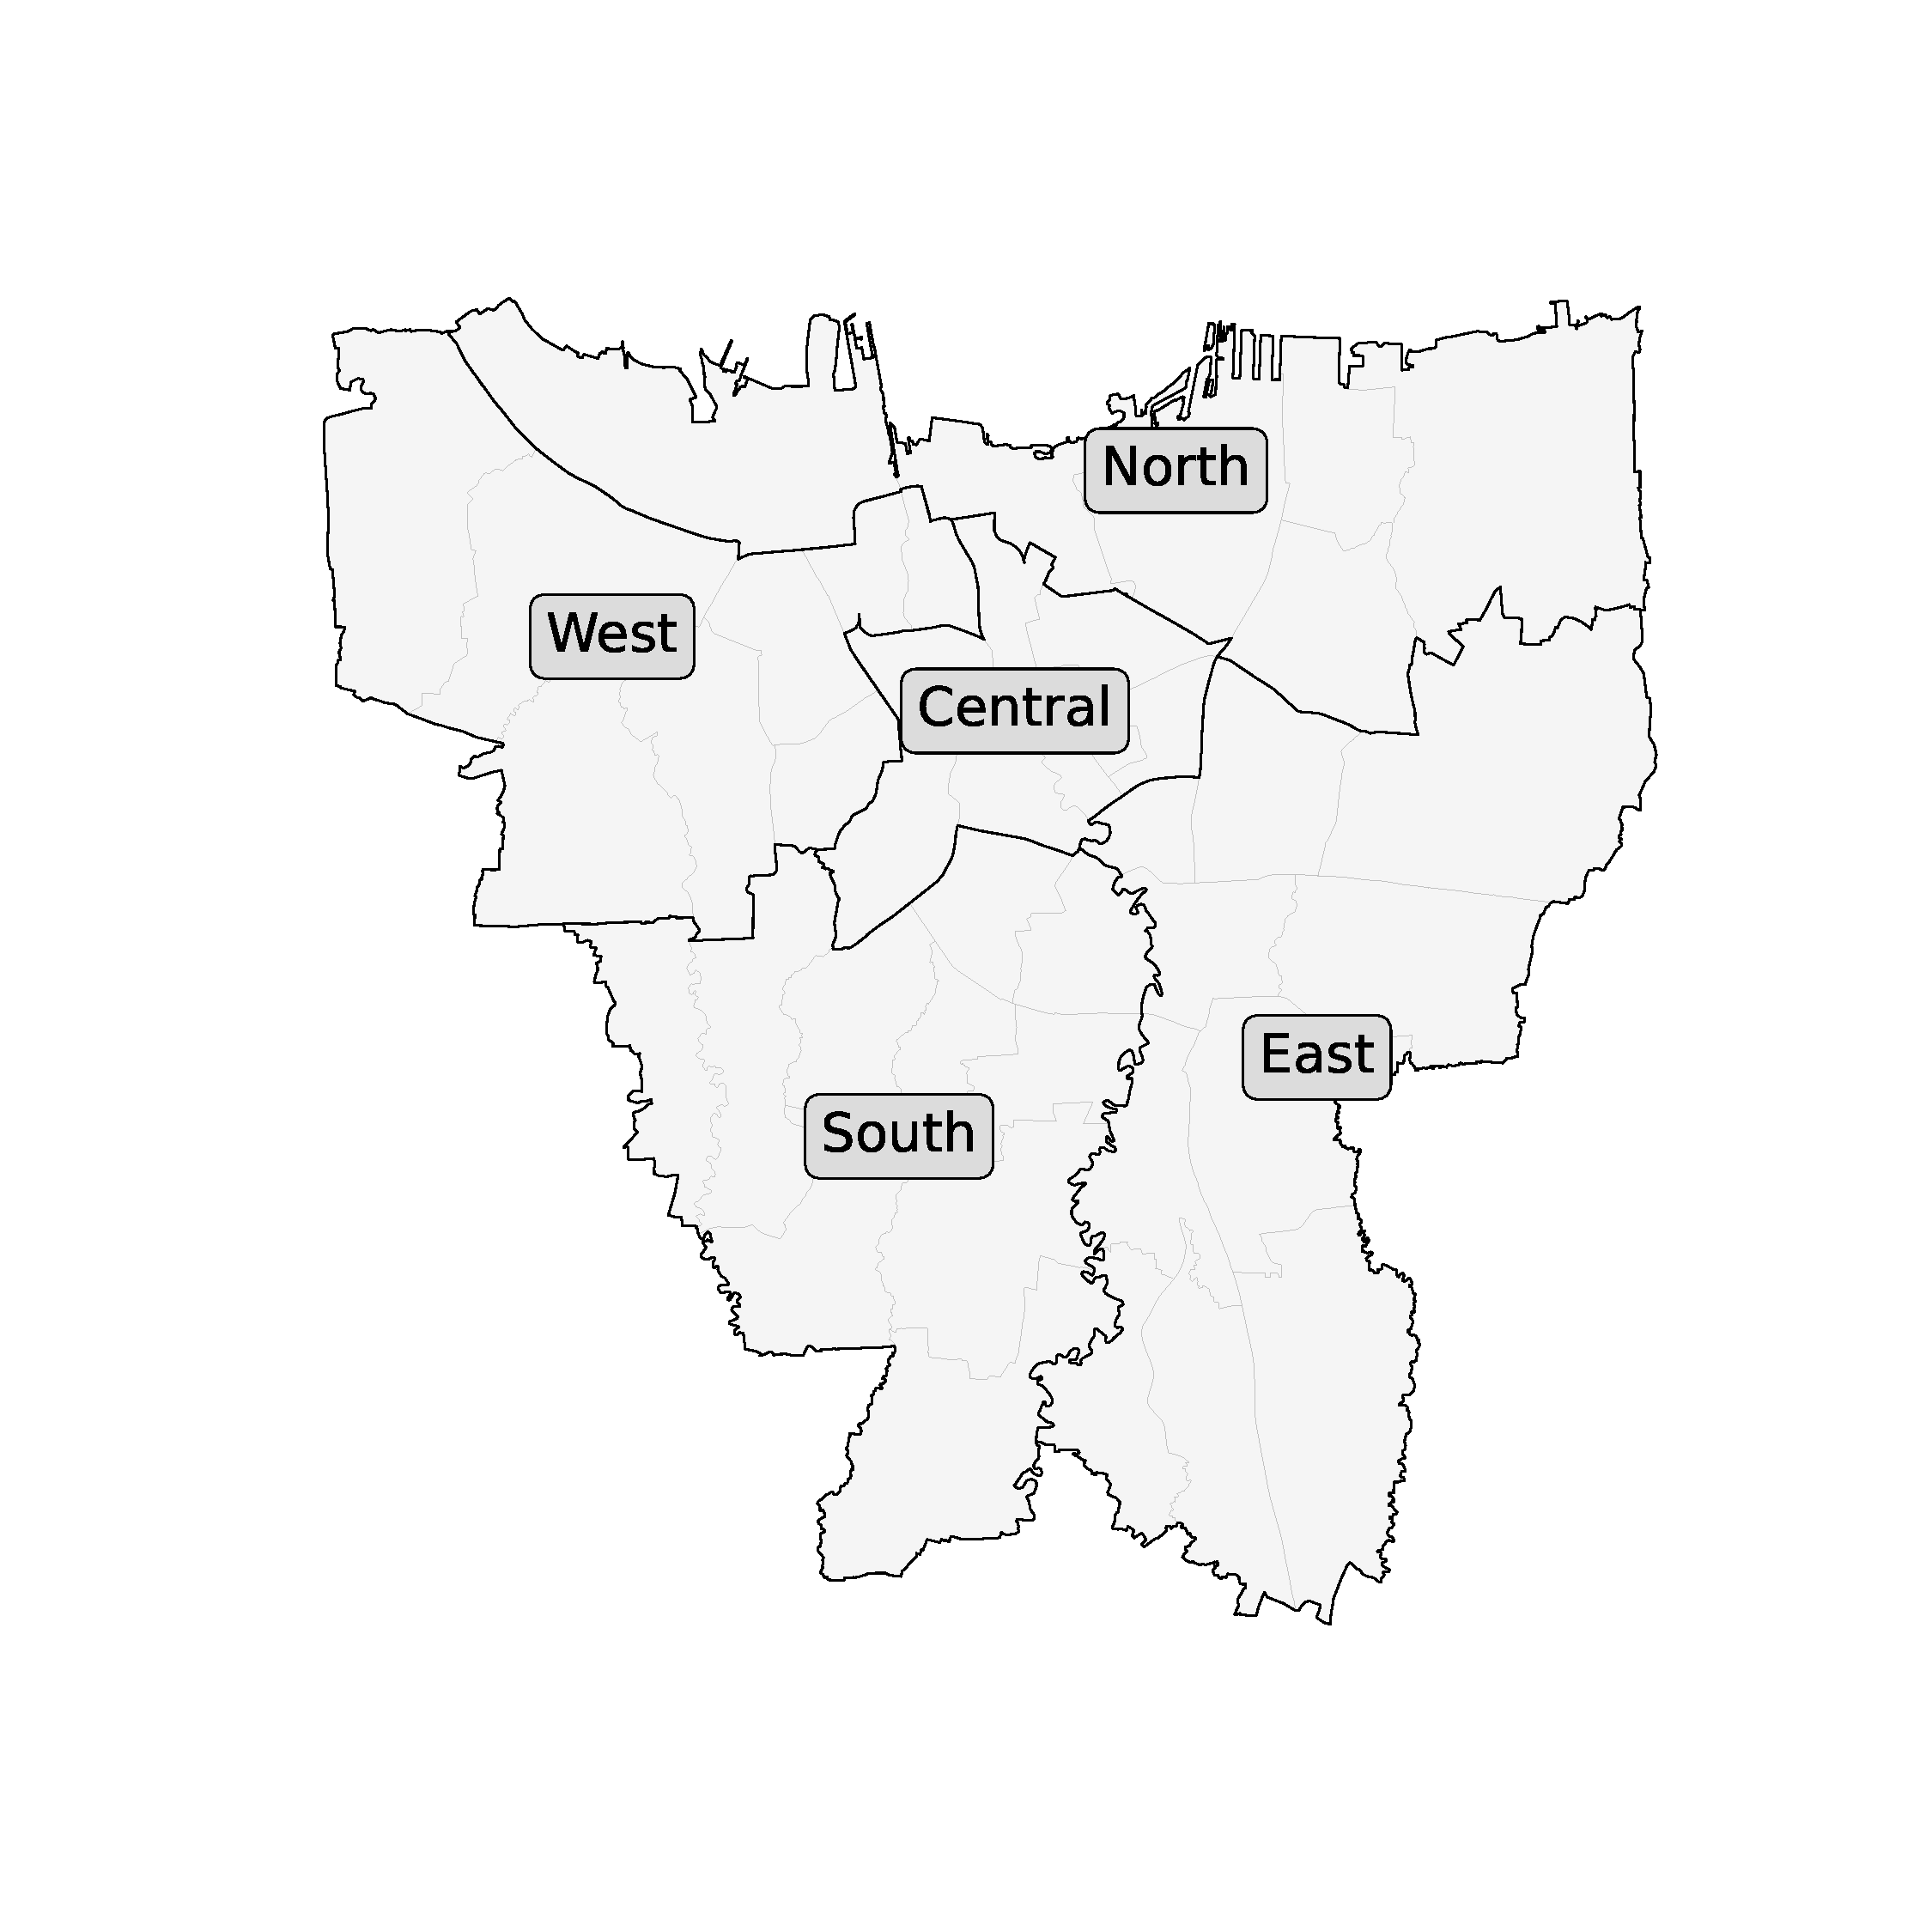
\includegraphics[width=0.8\textwidth]{img/jakarta_region_names.pdf} \end{center}
\caption{Map of Jakarta's Municipalities.} \label{fig:region_names} \end{figure}

\begin{itemize} \item \textbf{A1 - High priority emergency patients}: critical
            patients who require immediate life-saving assistance with a target
            ambulance response time of 8 minutes.  In our data set there were
            168 identified calls that met this criterion.  \item \textbf{A2 -
                Other emergency patients}: urgent patients that require
                assistance with a target response time of 15 minutes. In our
                data set there were 23,784 calls of this type.  \item \textbf{B
                    - Non-emergency patients}: patients that still benefit from
                    an ambulance response but non-critical with a target
                    response time of 60 minutes. There were 31,725 calls of this
                    type in the data set.  \end{itemize}

The number of calls from each of these specialities varies by neighbourhood, as
shown in Figure~\ref{fig:yearly_demand}. It can be seen that many calls are
highly concentrated in a handful of neighbourhoods rather than spread throughout
the city.

\begin{figure} \begin{center}
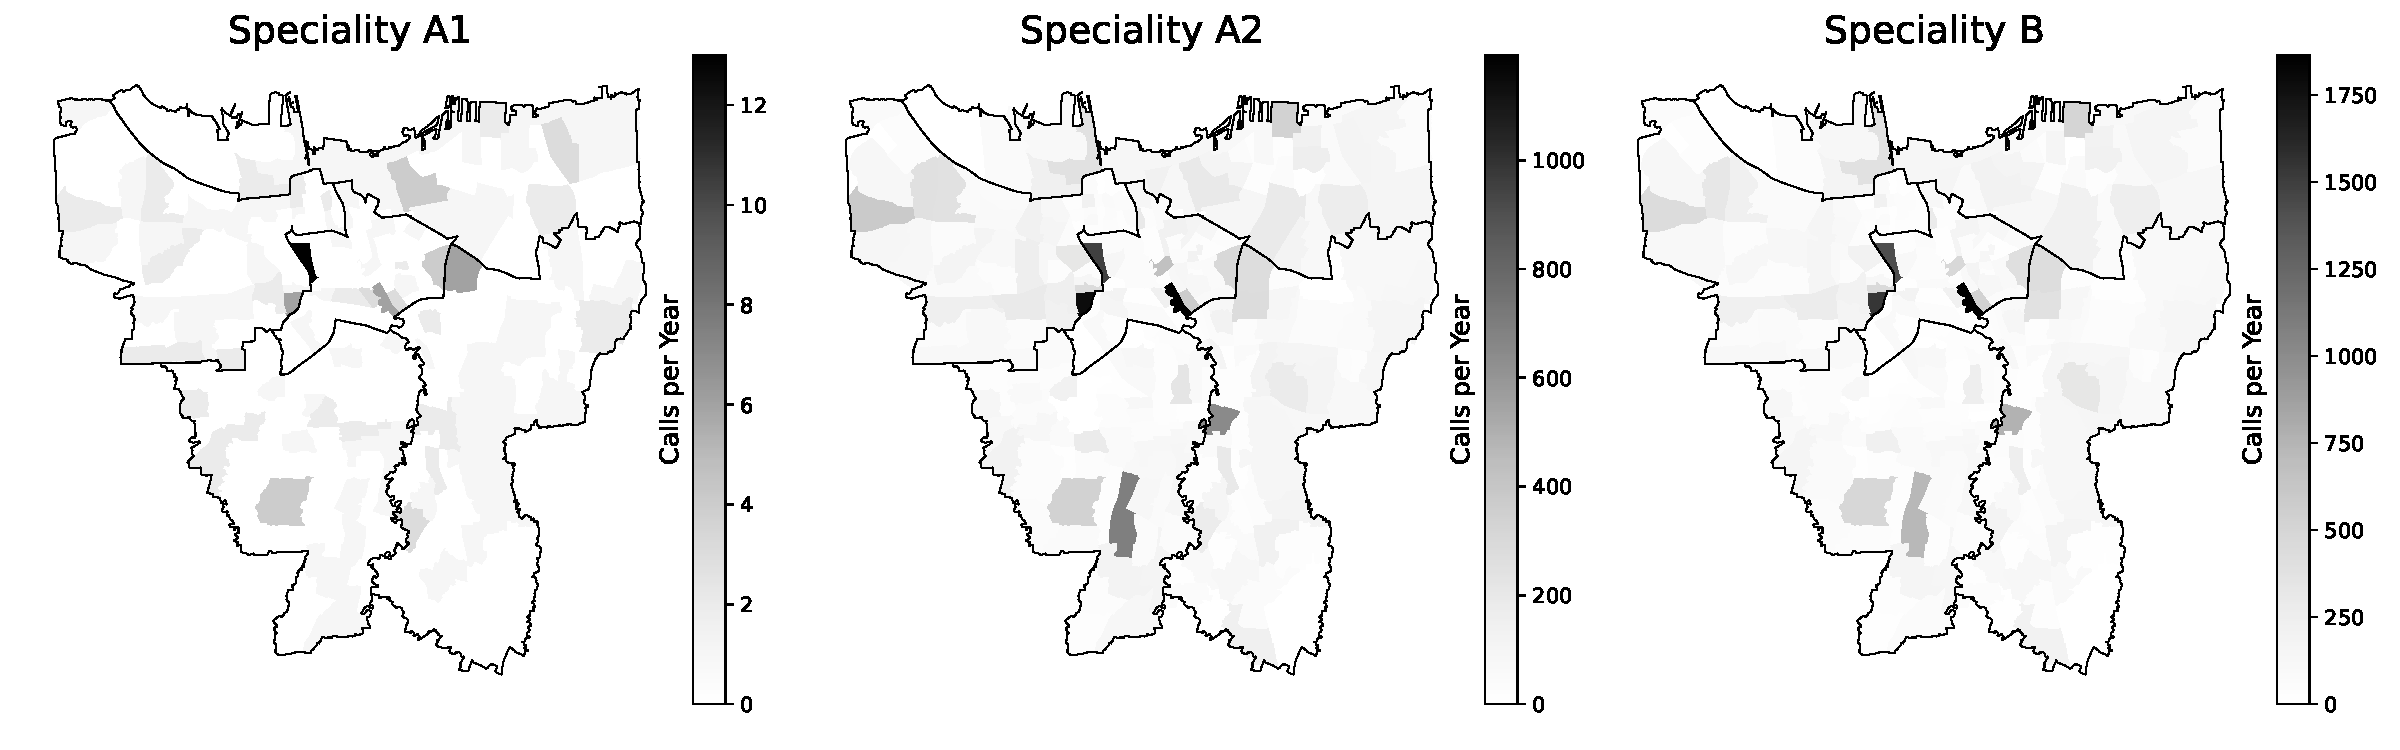
\includegraphics[width=\textwidth]{img/yearly_demand.pdf} \end{center}
\caption{Number of calls received by speciality and neighbourhood.}
\label{fig:yearly_demand} \end{figure}

In Sections~\ref{sec:analysis_current} and~\ref{sec:analysis_grid} we use the
discrete event simulation described above to find appropriate KPIs to measure
the performance of the current allocations and two proposed grid allocations for
the city. \ref{apx:parameters} provides further details on the parameterisation
of the model.

\begin{table} \begin{center} \begin{tabular}{ccc} \toprule Municipality & Number
    of neighbourhoods & Current number of ambulance stations \\ \midrule North
    & 31 & 9 \\ South   & 65 & 14 \\ East    & 63 & 13 \\ West    & 57 & 16 \\
    Central & 45 & 15 \\ \bottomrule \end{tabular} \caption{Numbers of
    neighbourhoods and ambulance stations by municipality.} \label{tbl:jakarta}
    \end{center} \end{table}

\subsection{Survival Functions}\label{sec:survival} A key concept here is the
survival curve of a patient.  In reality, some emergency incidents do not result
in a substantive deterioration of a patient’s status over time; however, in all
situations, there is a reasonable cut-off beyond which a patient should not
expect to have to wait for care, and mixture of theoretical survival functions
and step functions can be utilised.  Survival probabilities for critical
incidents, calculated from a theoretical monotonically decaying survival
function reported in the literature \cite{Valenzuela20001206} are used to
demonstrate an attainable level of success from a response. One particular
survival curve $s_1(t)$ of Equation~\ref{eqn:survival_curve}, represents
survival until hospital discharge following cardiac arrest; its origins are
explained in detail by \cite{Knight2012918}. It is used here for critical A1
patients. Figure~\ref{fig:survivalfunction} shows the difference between using
this survival curve and a hard cut-off of 8 minutes.  However, hard cut-off
curves like Equation~\ref{eqn:survival_cutoff_8} can still be used to represent
meeting artificially selected targets and are used here for the survival of A2
and B patients, with targets of 15 and 60 minutes respectively, given by
Equations~\ref{eqn:survival_cutoff_15} and~\ref{eqn:survival_cutoff_60}.

\begin{equation}\label{eqn:survival_curve} s_1(t) = \left(1 +
e^{0.26+0.139t}\right)^{-1} \end{equation}

\begin{equation}\label{eqn:survival_cutoff_8} s_2(t) = \begin{cases} 1 \text{ if
} 0\leq t \leq 8 \\ 0 \text{ if } t > 8 \end{cases} \end{equation}

\begin{equation}\label{eqn:survival_cutoff_15} s_3(t) = \begin{cases} 1 \text{
if } 0\leq t \leq 15 \\ 0 \text{ if } t > 15 \end{cases} \end{equation}

\begin{equation}\label{eqn:survival_cutoff_60} s_4(t) = \begin{cases} 1 \text{
if } 0\leq t \leq 60 \\ 0 \text{ if } t > 60 \end{cases} \end{equation}

\begin{figure}[ht] \centering
    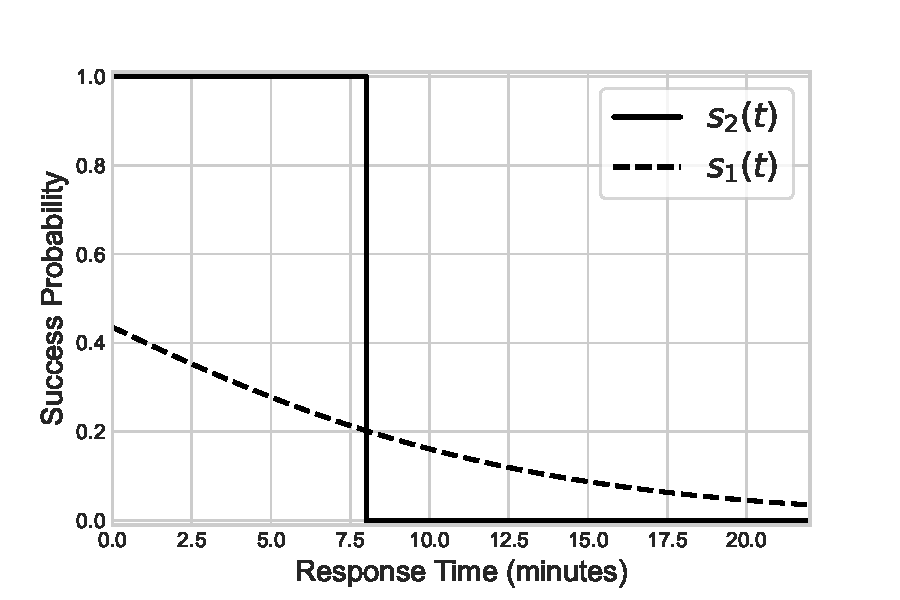
\includegraphics[width=0.6\textwidth]{img/Survival_Function_(new).pdf}
    \caption{Survival function $s_1(t)$, estimated by \cite{Valenzuela20001206}
    compared with a current EMS target, $s_2(t)$, represented as a step function
    (binary coverage).} \label{fig:survivalfunction} \end{figure}


\subsection{Current Allocation}\label{sec:analysis_current} As of October 2022,
the 119 service in Jakarta ran a fleet of 81 primary Emergency Ambulances (EAs)
and 13 secondary motorbike Rapid Response Vehicles (RRVs), distributed across 67
ambulance stations throughout the city. Table~\ref{tbl:jakarta} and
Figure~\ref{fig:current_allocation} summarise the allocations by municipality
and sub districts. 

\begin{figure} \begin{center}
    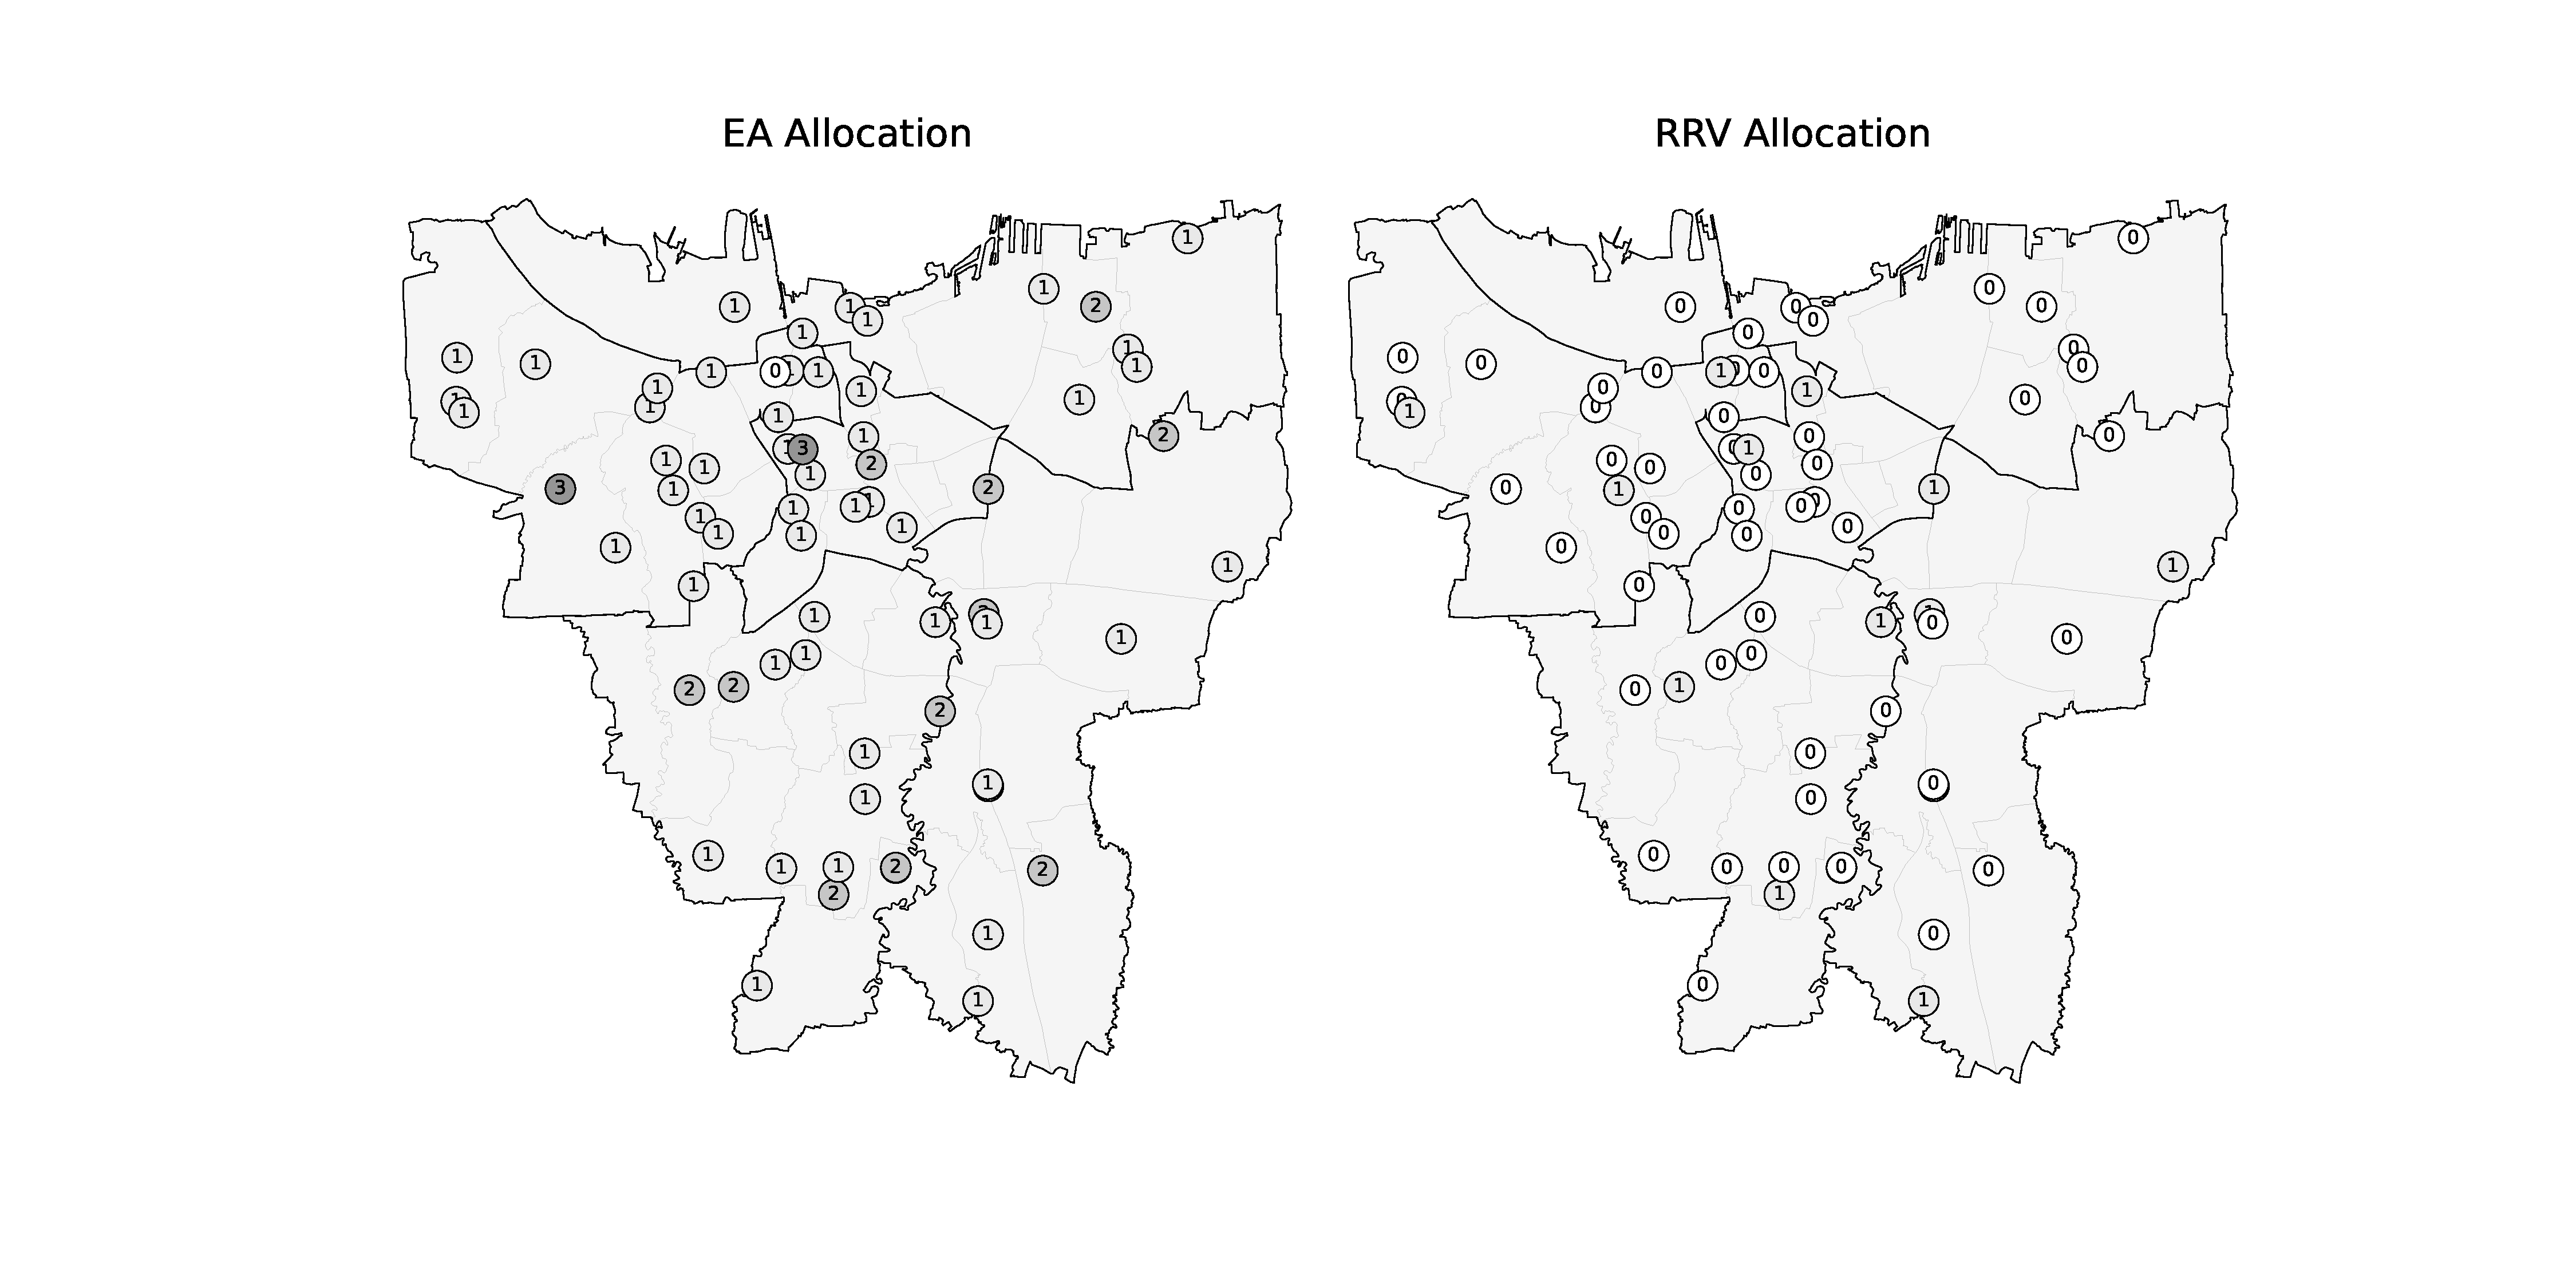
\includegraphics[width=\textwidth]{img/map_current} \caption{Map of current
    Emergency Ambulance (EA) and Rapid Response Vehicle (RRV) locations and
    allocations to ambulance bases across Jakarta.}
    \label{fig:current_allocation} \end{center} \end{figure}

\subsection{Proposed `Grid' Allocation}\label{sec:analysis_grid} Discussions
with senior staff at 119 identified that they were seriously considering to
re-configure their ambulance allocations into a grid structure, placing an
ambulance station at regular intervals throughout the city and uniformly
distributing the vehicles that they felt would ensure coverage. Two possible
grid allocations were being considered: one placing an EA every 3km across the
city (giving a total of 70 vehicles), and another placing three EAs every 5km
across the city (giving a total of 72 vehicles).
Figure~\ref{fig:grid_allocations} show these proposed allocations.

\begin{figure} \begin{center} \begin{subfigure}{0.48\textwidth}
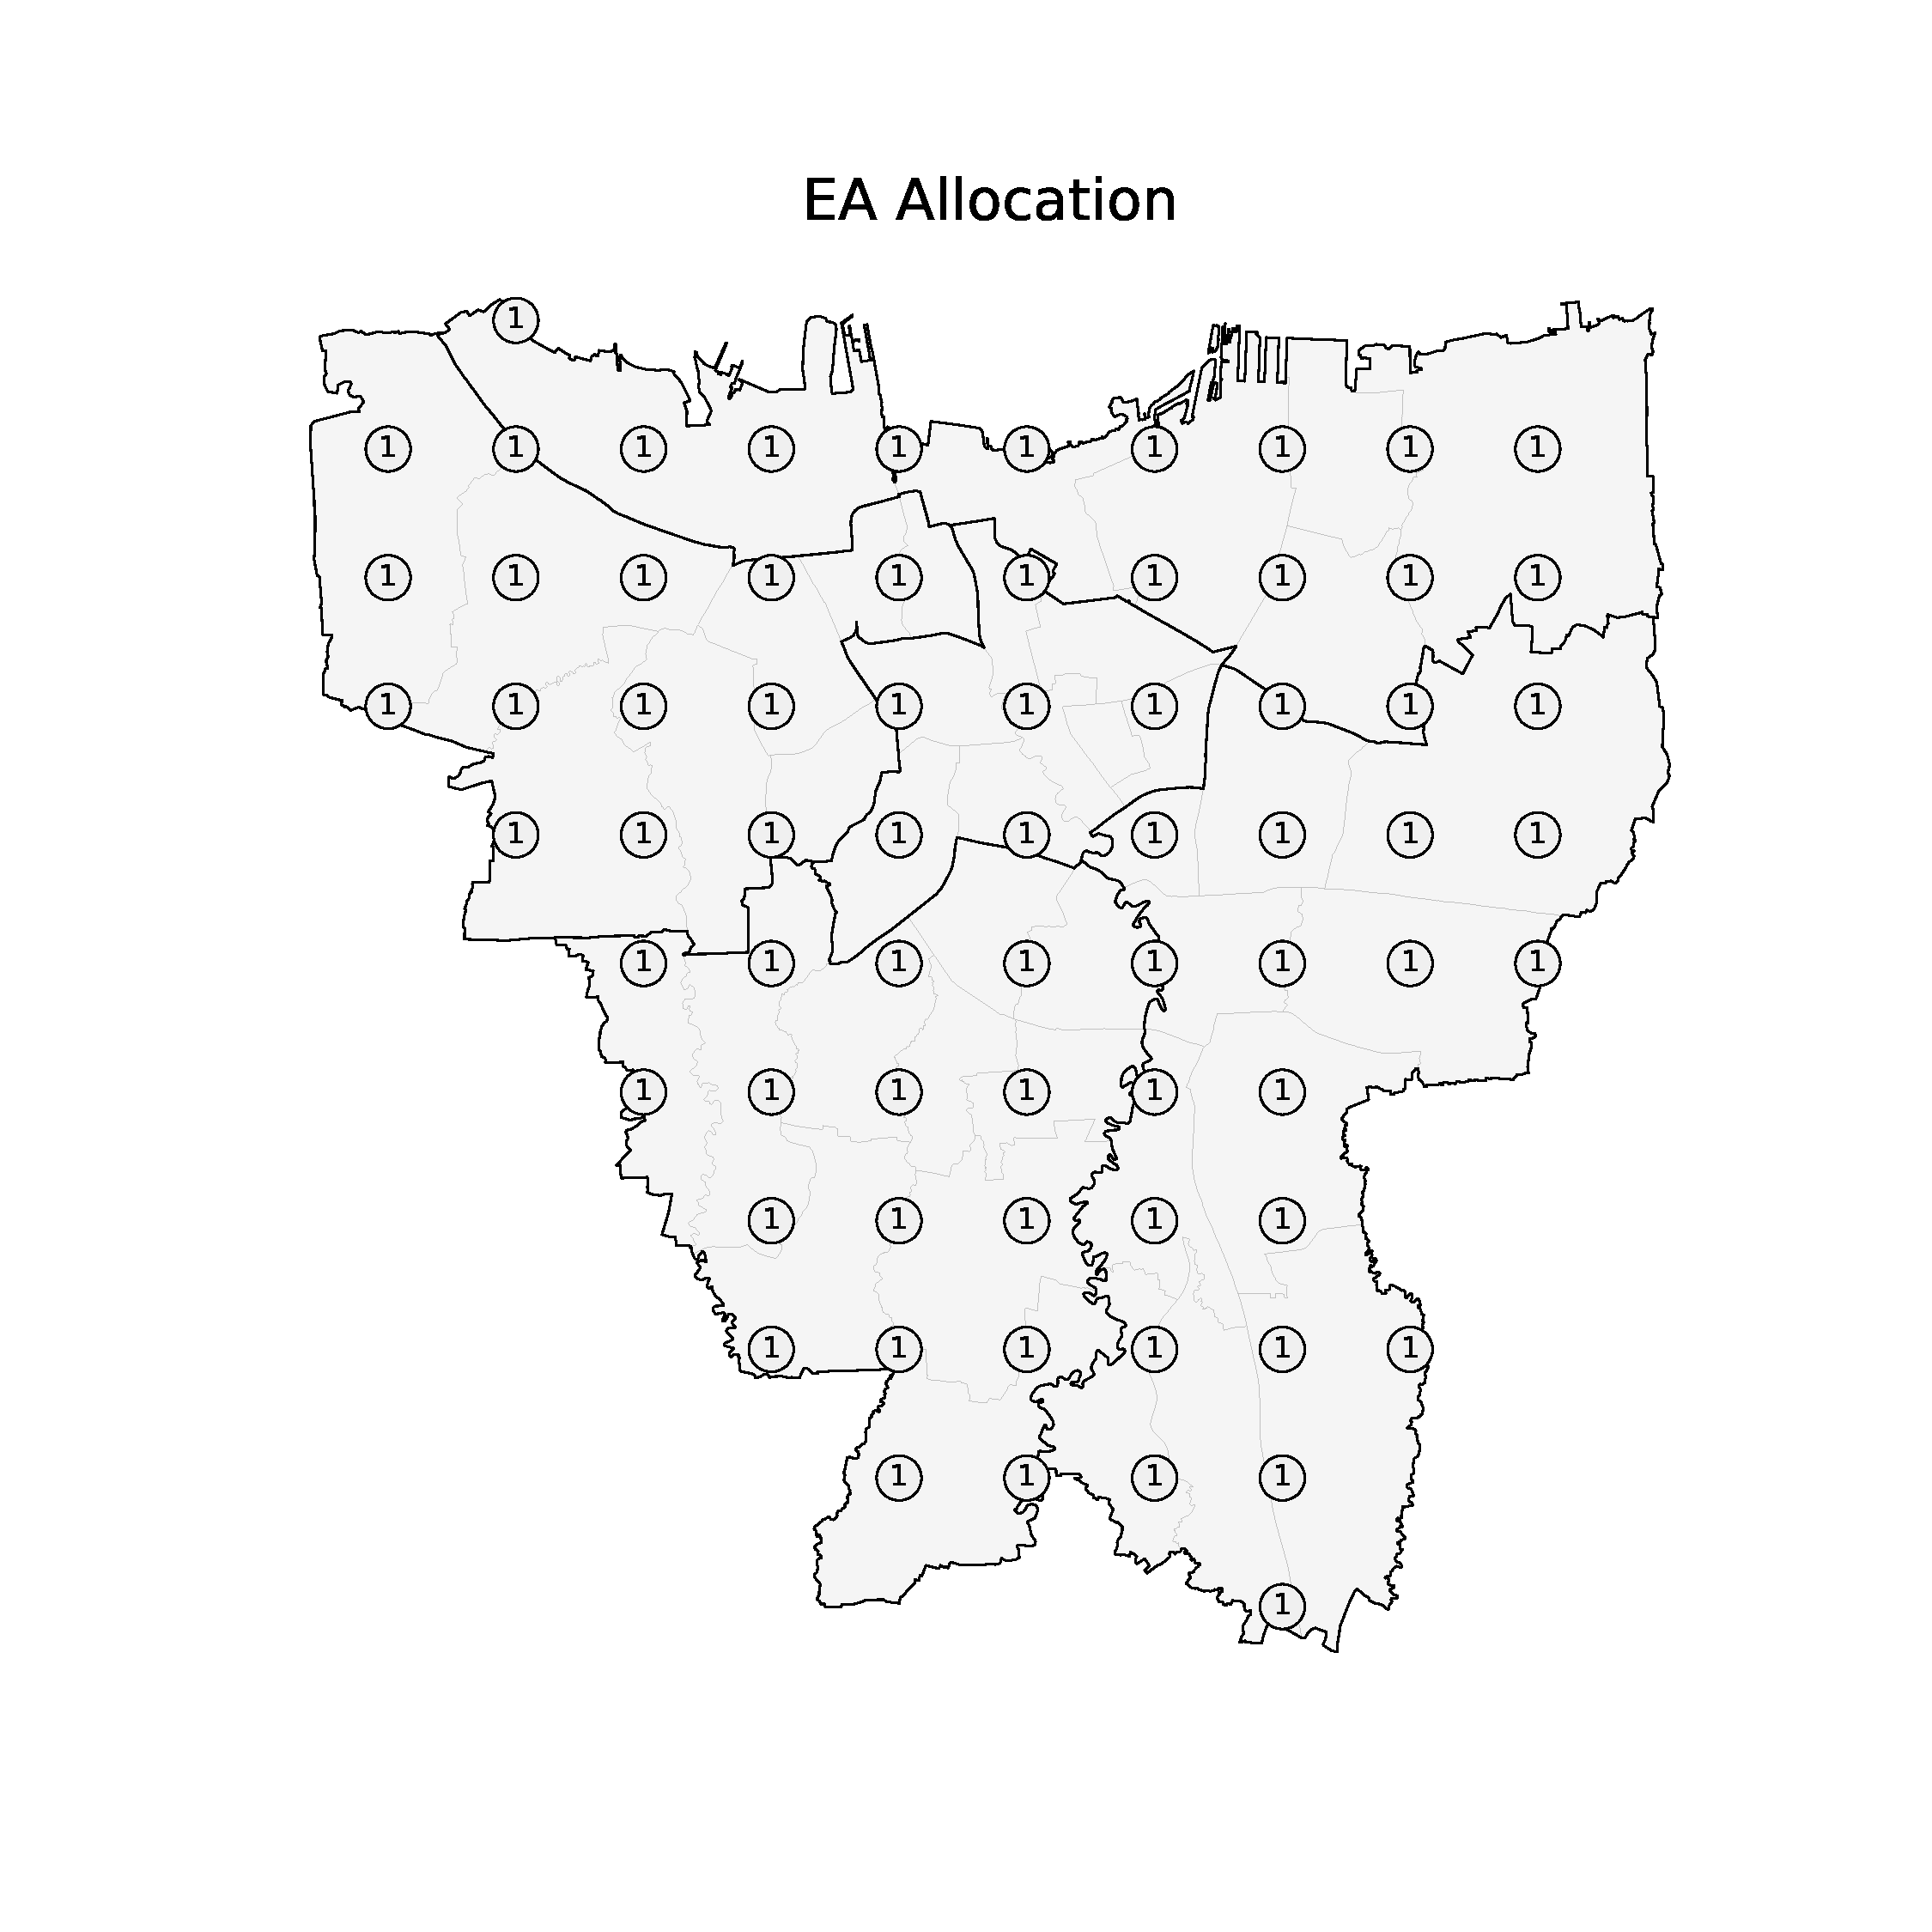
\includegraphics[width=\textwidth]{img/map_grid3km_proposed} \caption{3km grid.}
\end{subfigure} \hfill \begin{subfigure}{0.48\textwidth}
    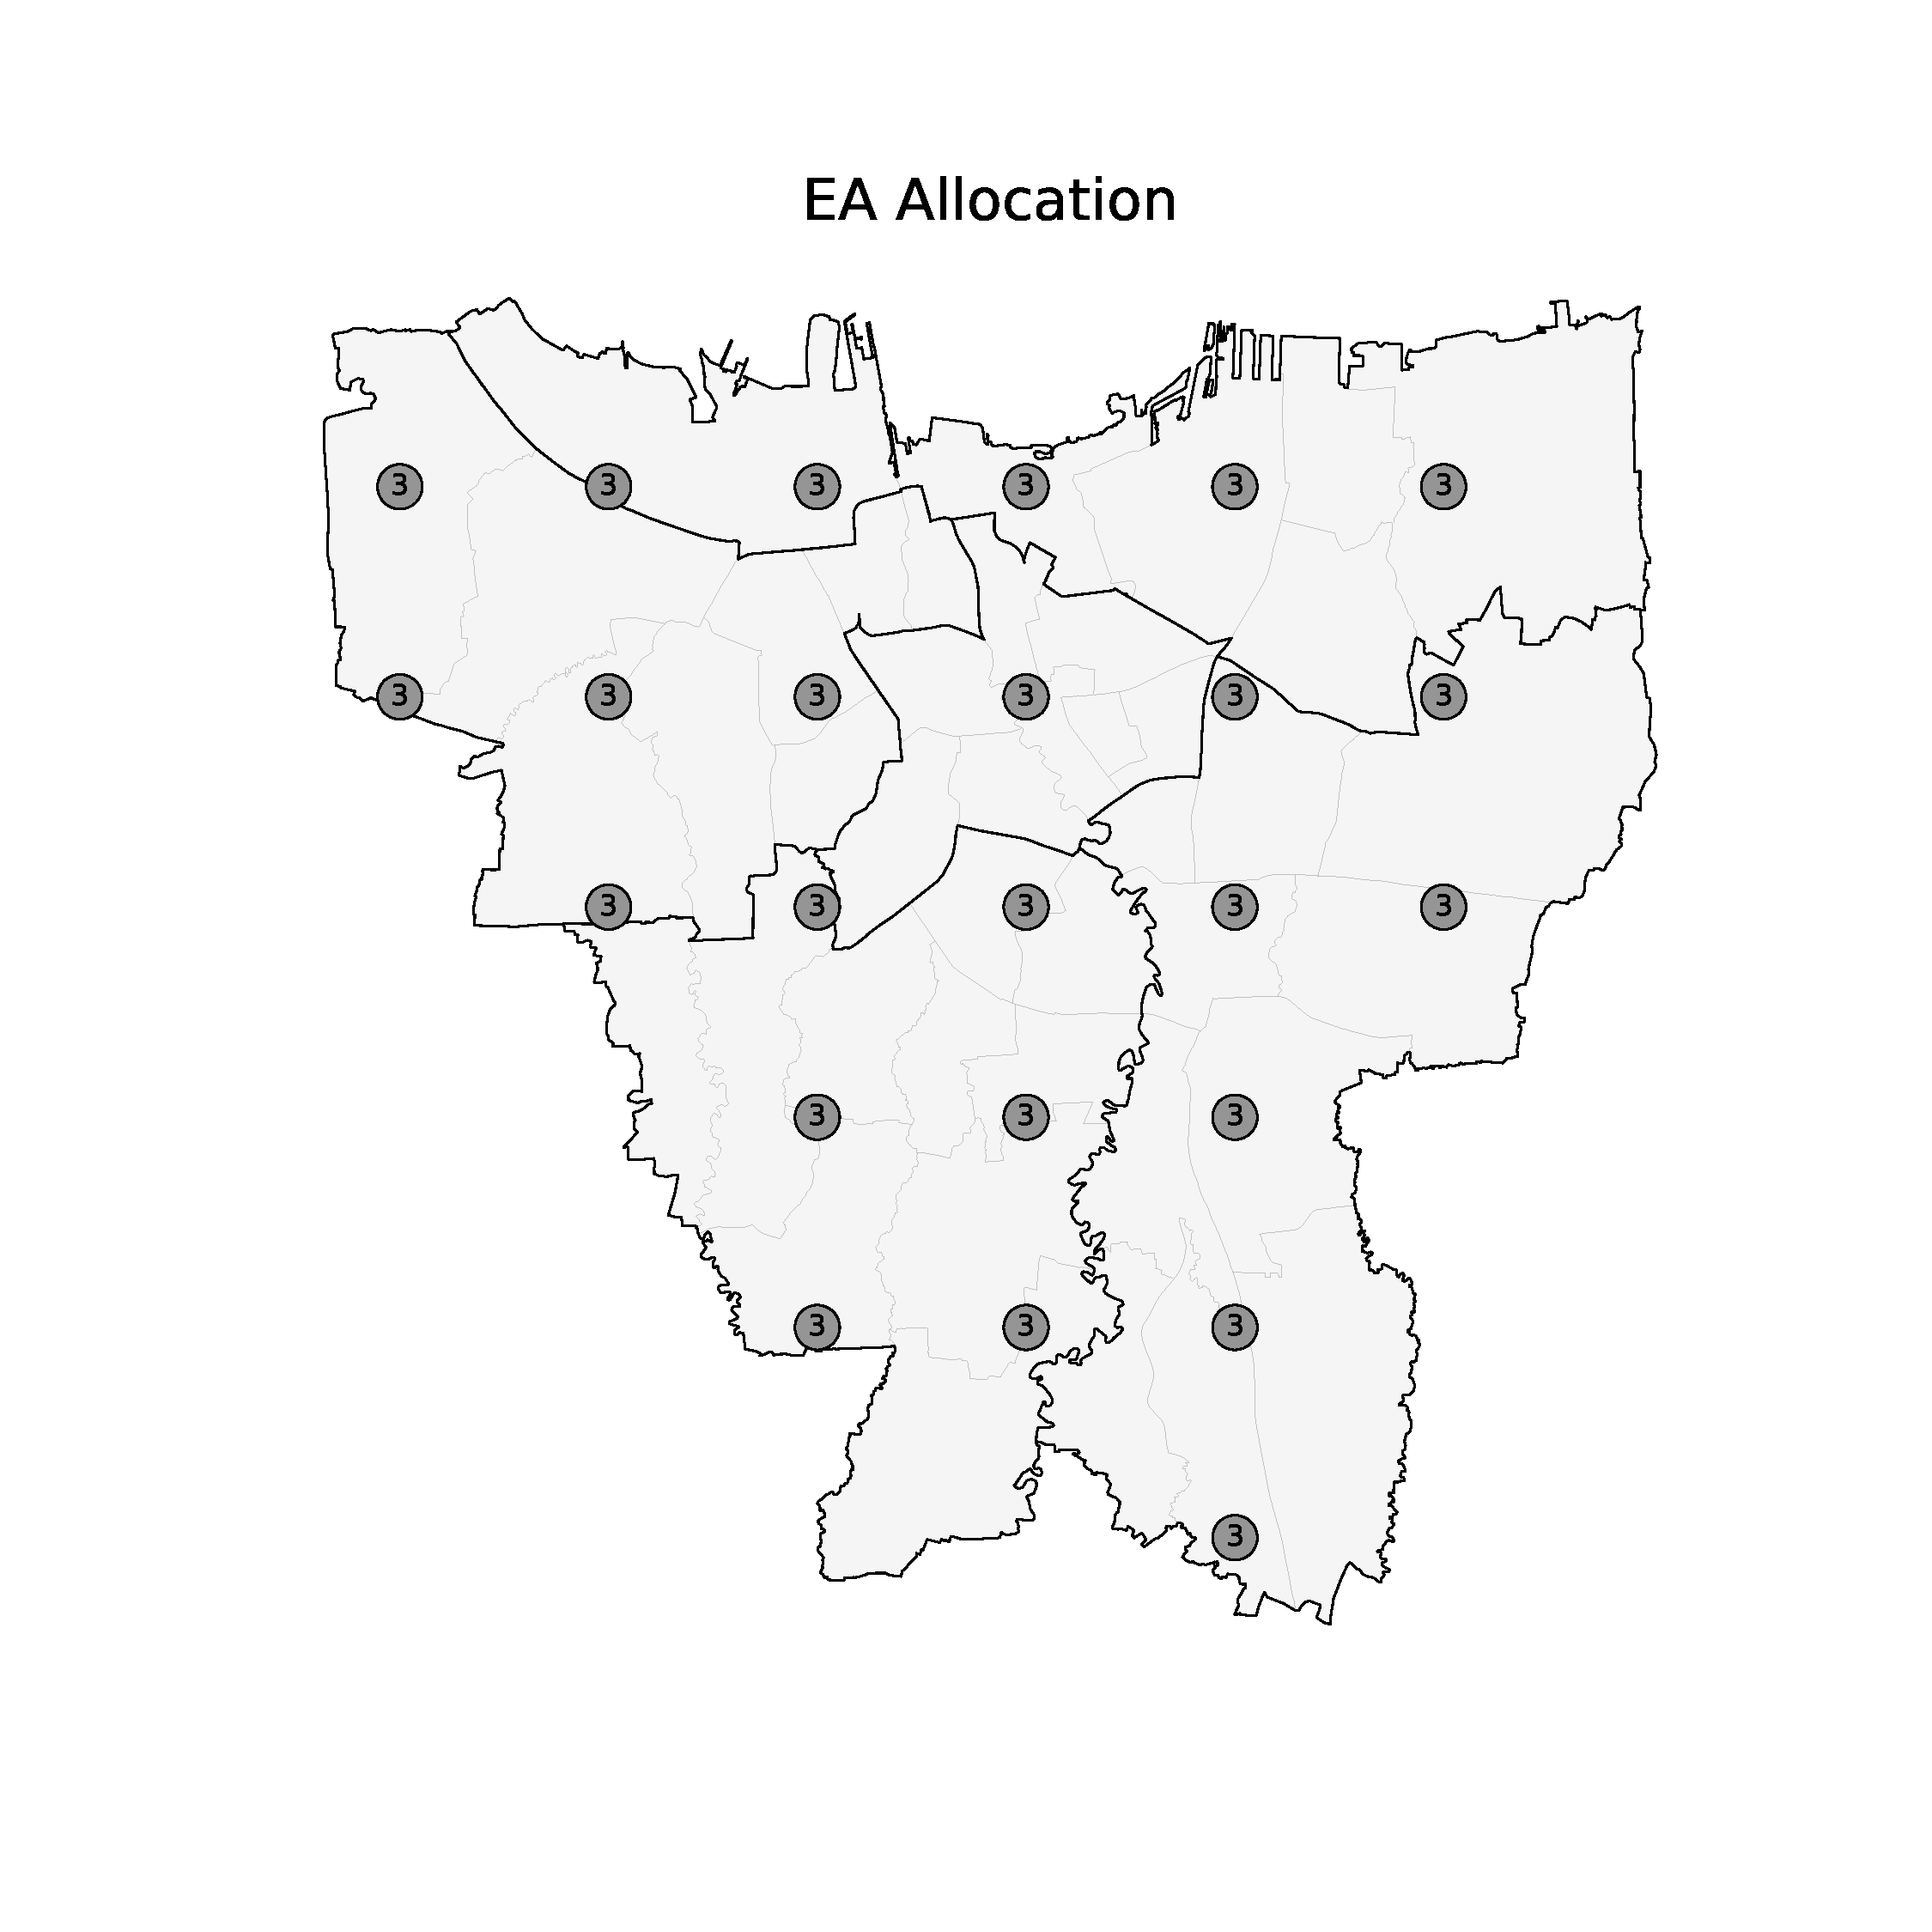
\includegraphics[width=\textwidth]{img/map_grid5km_proposed} \caption{5km
grid.} \end{subfigure} \caption{Proposed grid allocations.}
\label{fig:grid_allocations} \end{center} \end{figure}

\begin{table} \begin{center} \begin{tabular}{rrrr} \toprule Allocation &
    Baseline & Grid 3km & Grid 5km \\ \midrule Number of EAs & 81 & 70 & 71 \\
    Number of RRVs & 13 & 0 & 0 \\ Ambulance Utilisation & 31.7\% & 37.4\% &
    36.6\% \\ RRV Utilisation & 40.9\% & - & - \\ Mean Response Time (mins) &
    16.80 & 22.39 & 24.14 \\ Overall Survival & 75.5\% & 63.7\% & 61.0\% \\
    Percent Abandoned & 0.034\% & 0.430\% & 1.028\% \\ \bottomrule \end{tabular}
    \caption{Calculated KPIs for the current and proposed grid allocations.}
    \label{tbl:current_grid_results} \end{center} \end{table}

The simulation was run for both current  and proposed grid allocations and
results are shown and compared in Table~\ref{tbl:current_grid_results}.  We
observe that the two proposed grid allocations perform much worse than the
current allocation as measured by mean response time, survival, and percentage
of calls abandoned.

\subsection{Planning for Future Demand}\label{sec:demand_scenarios} Similarly to
many other cities worldwide, ambulance services in Jakarta anticipate that
demand for services will grow in future years, not least that there is now a
coordinated service accessible via a single common number `119' to call. This
should help raise awareness and visibility of an ambulance service. In the case
of Jakarta, certainly increased use of 119 and therefore increased demand would
be a desired outcome resulting from proactive actions by the Indonesian
Government. 

We consider four different demand scenarios, developed by considering the result
of our cross-sectional study of patients attending EDs in Jakarta
\cite{BriceSyaribahNoor2022Esui}. As part of the survey, randomly selected
patients arriving at each emergency department were asked whether they had used
an ambulance to attend, and reasons for not using an ambulance. For those
patients who were categorised by the medical staff as emergency and for whom
therefore an ambulance might have seemed a sensible option, the responses are
given in Table~\ref{table:survey_results}.

\begin{table} \centering \begin{tabular}{rr} \toprule Reason & \% of emergency
    respondents \\

\midrule Used Ambulance & 13.0\\ Too expensive & 5.2  \\ Not available  & 13.1
    \\ Would take too long & 16.5 \\ Not necessary & 15.7  \\ Not aware of
    service & 33.1\\ Other &3.5 \\

 \bottomrule \end{tabular} \caption{Barriers to use of an ambulance service in
 Jakarta, from \cite{BriceSyaribahNoor2022Esui}.} \label{table:survey_results}
 \end{table}

The survey confirmed three major barriers to use, namely: the service's
visibility (33.1\% of respondents were unaware of the service), the service's
reliability (13.1\% of respondents reported that there was no ambulance
available and 16.5\% of respondents believed it would take too long), and the
service's cost (5.2\% of respondents cited cost as a deterrent). Therefore, four
demand scenarios were considered, corresponding to addressing each of these
barriers in turn:

\begin{itemize} \item \textbf{demand\_13}: this represents the current situation
            where approximately 13\% of emergency patients (specialities A1 and
        A2) do use an ambulance.  \item \textbf{demand\_19}: this represents the
            situation where visibility is addressed. Here, we distribute the
            33.1\% of the respondents who were unaware of the service
            proportionally between using the ambulance and amongst the remaining
            issues. Using this methodology we would expect 19.4\% of emergency
            patients to now use an ambulance.  \item \textbf{demand\_34}: this
                represents the situation where reliability and visibility are
                addressed. Using the same methodology we would expect 34.8\% of
                emergency patients to now use an ambulance.  \item
                    \textbf{demand\_45}: this represents the situation where
                    cost, reliability and visibility are all addressed. Using
                    the same methodology we would expect 45.4\% of emergency
                    patients to now use an ambulance.  \end{itemize}

Guided by our findings in \cite{BriceSyaribahNoor2022Esui}, recent changes mean
that the 119 services is now free to use for Jakarta residents, so certainly the
highest demand (demand\_45) scenario is plausible in the near future.  After
discussions with our partners, it was agreed that for each of the scenarios we
should assume that non-emergency demand (speciality B) remains unchanged.  

Table~\ref{tbl:demand_results} gives the derived KPIs for the current allocation
for each of these demand scenarios in the simulation. In all measured KPIs, the
performance worsens as emergency demand increases, thus motivating the need to
find better allocations and investigate the effect of varying resource levels
and explict consideration of patient outcomes, detailed in
Section~\ref{sec:betterallocations}.

\begin{table} \begin{center} \small \begin{tabular}{rrrrr} \toprule Demand
    Scenario & \textbf{demand\_13} & \textbf{demand\_19} & \textbf{demand\_34} &
    \textbf{demand\_45} \\ \midrule Ambulance Utilisation & 31.7\% & 38.9\% &
    54.9\% & 62.5\% \\ RRV Utilisation & 40.9\% & 47.7\% & 62.3\% & 68.5\% \\
    Mean Response Time (mins) & 16.80 & 17.98 & 22.18 & 23.97 \\ Overall
    Survival & 75.5\% & 67.7\% & 52.6\% & 46.0\% \\ Percent Abandoned & 0.034\%
    & 0.315\% & 3.910\% & 10.004\% \\ \bottomrule \end{tabular}
    \caption{Calculated KPIs for the current allocation under the four possible
    demand scenarios.} \label{tbl:demand_results} \end{center} \end{table}


\section{Finding Better Allocations}\label{sec:betterallocations} In this
section we propose a heuristic approach of finding ambulance allocations for a
given resource level. A cross-entropy optimisation approach is used to find
allocations that maximise the expected survival of the patients served. These
allocations are also simulated using the developed simulation  described in
Section~\ref{sec:simulation} and demonstrated in Section~\ref{sec:jakarta}, to
obtain their equivalent simulation based KPIs.

First, in Section~\ref{sec:objective_function} a maximal expected survival score
is given for heterogeneous patients and heterogeneous vehicles, to be used an
objective function. Then in Section~\ref{sec:cross_entropy} a cross-entropy
heuristic algorithm is described to find better fleet allocations, while
Section~\ref{sec:experiment} describes the design of the numerical experiments
across the relevant scenarios. Section~\ref{sec:optimisation_results} provides
the results of the optimisation based on the KPIs obtained through the discrete
event simulation.


\subsection{MESLMHPHF Objective Function}\label{sec:objective_function} The
intent of the objective function used for the heuristic optimisation algorithm
is to maximise patient survival. Here we formulate a weighted expected survival
function as the objective function which considers heterogeneous patients
(different specialities) and heterogeneous fleets (both primary vehicles, EAs,
and secondary vehicles, RRVs), called the Maximal Expected Survival Location
Model with Heterogeneous Patients and Heterogeneous Fleet (MESLMHPHF). It is an
extension of the MESLMHP model given in \cite{Knight2012918}, which did not
consider heterogeneous fleets.

% A key concept here is the survival curve of a patient.  In reality, some
% emergency incidents do not result in a substantive deterioration of a
% patient’s status over time; however, in all situations, there is a reasonable
% cut-off beyond which a patient should not expect to have to wait for care, and
% mixture of theoretical survival functions and step functions can be utilised.
% Survival probabilities for critical incidents, calculated from a theoretical
% monotonically decaying survival function reported in the literature
% \cite{Valenzuela20001206} are used to demonstrate an attainable level of
% success from a response. One particular survival curve $s_1(t)$ of
% Equation~\ref{eqn:survival_curve}, represents survival until hospital
% discharge following cardiac arrest; its origins are explained in detail by
% \cite{Knight2012918}. It is used here for critical A1 patients.
% Figure~\ref{fig:survivalfunction} shows the difference between using this
% survival curve and a hard cut-off of 8 minutes.  However, hard cut-off curves
% like Equation~\ref{eqn:survival_cutoff} can still be used to represent meeting
% artificially selected targets and are used here for the survival of A2 and B
% patients, with targets of 15 and 60 minutes respectively.

% \begin{equation}\label{eqn:survival_curve} s_1(t) = \left(1 +
% e^{0.26+0.139t}\right)^{-1} \end{equation}

% \begin{equation}\label{eqn:survival_cutoff} s_2(t) = \begin{cases} 1 \text{ if
% } 0\leq t \leq 8 \\ 0 \text{ if } t > 8 \end{cases} \end{equation}

% \begin{figure}[ht] \centering
% 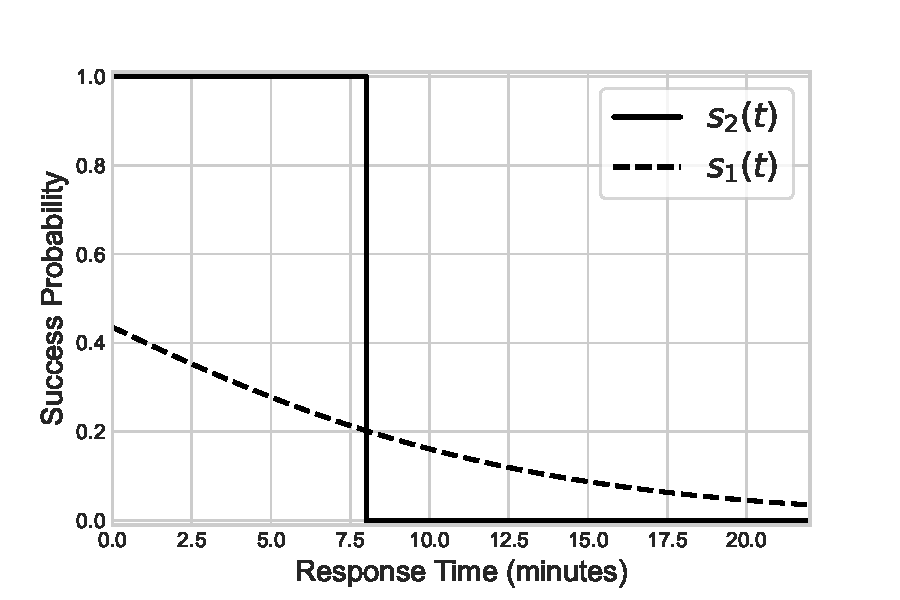
\includegraphics[width=0.6\textwidth]{img/Survival_Function_(new).pdf}
% \caption{Survival function $s_1(t)$, estimated by \cite{Valenzuela20001206}
% compared with a current EMS target, $s_2(t)$, represented as a step function
% (binary coverage).} \label{fig:survivalfunction} \end{figure}

Our maximal survival function is constructed by appropriately summing these
survival curves, described in Section~\ref{sec:survival}, across the population,
multiplying by ambulance availability where appropriate.  We let $Z_a$ and
$\tilde{Z}_a$ denote the number of primary vehicles and secondary vehicles at
ambulance station $a$, respectively, that is, the allocation. To incorporate
heterogeneous fleets, as was modelled by the simulation in
Section~\ref{sec:simulation}, the set of specialities $\mathcal{K}$ is
partitioned into two sets, $\mathcal{K}_A$, those patients that can be seen by
secondary vehicles (in the Jakarta case including specialities A1 and A2), and
$\mathcal{K}_B$, those patients who are seen by primary vehicles only (in the
Jakarta case including speciality B only). Then, the MESLMHPHF objective
function is given by Equation~\ref{eqn:meslmhphf},

\begin{equation}\label{eqn:meslmhphf} g\left(Z_a, \tilde{Z}_a\right) = \sum_{p
    \in \mathcal{P}} \sum_{a \in \mathcal{A}} \left( \sum_{k \in \mathcal{K}_A}
    w_k \lambda_{pk} \hat{\Psi}_{kpa} + \sum_{k \in \mathcal{K}_B}  w_k
    \lambda_{pk} \Psi_{kpa} \right) \end{equation}

where $w_k$ is a weight associated with patient speciality type $k$ (for this
study we assume $w_k = 1$ for all $k$), $\lambda_{pk}$ is the rate of demand of
patients of speciality $k$ at pick-up location $p$. Now $\Psi_{kpa}$ is the
expected survival of patients of speciality $k \in \mathcal{K}_B$ at location
$p$ from station $a$, while $\hat{\Psi}_{kpa}$ is the expected survival of
patients of speciality $k \in \mathcal{K}_A$ at location $p$ from station $a$.
Equation~\ref{eqn:meslmhphf} is the weighted sum over the expected survival
functions of all patient specialities, all patient pick-up locations, and all
ambulance stations. These expected survival functions are given by
Equations~\ref{eqn:survival_A} and~\ref{eqn:survival_B} respectively,

\begin{equation}\label{eqn:survival_A} \Psi_{kpa} = s_k\left( t_{pa} \right)
\left(1 - \pi_{a}^{Z_a} \right) \prod_{\alpha \in \mathcal{A}}
\pi_{\alpha}^{\left(Z_{\alpha} \beta_{p\alpha a} \right)} \end{equation}

\begin{align}\label{eqn:survival_B} \hat{\Psi}_{kpa} &=
    s_k\left(\hat{t}_{pa}\right) \left(1 - \tilde{\pi}_{a}^{\tilde{Z}_a} \right)
    \prod_{\alpha \in \mathcal{A}}
    \tilde{\pi}_{\alpha}^{\left(\tilde{Z}_{\alpha} \beta_{p\alpha a}\right)}
    \pi_{\alpha}^{\left(Z_{\alpha} R_{p \alpha a}\right) } \nonumber \\ &+
    s_k\left(t_{pa}\right) \left(1 - \pi_{a}^{Z_a} \right) \prod_{\alpha \in
    \mathcal{A}} \pi_{\alpha}^{\left(Z_{\alpha}\beta_{p\alpha a}\right)}
    \tilde{\pi}_{\alpha}^{\left(\tilde{Z}_{\alpha} \left(1 - R _{p
    a\alpha}\right)\right)} \end{align}

% TODO Modify the text after modifactions made to the above equation (for
    % example: we no longer need Q).

Here $s_k$ denotes the survival functions of patients of speciality $k$
(Equation~\ref{eqn:survival_curve} when $k$ represents A1 patients, and
Equations~\ref{eqn:survival_cutoff_15} and~\ref{eqn:survival_cutoff_60} when $k$
represents A2 and B patients respectively); $t_{pa}$ and $\hat{t}_{pa}$ denote
the expected time to travel from $a$ to $p$ for primary vehicles and secondary
vehicles respectively; and $\pi_{a}$ and $\tilde{\pi}_{a}$ is the utilisation at
ambulance station $a$ of primary and secondary vehicles respectively.  $R_{p a_1
a_2}$ and $\beta_{p a_1 a_2}$ are binary variables indicating the preference of
sending a vehicle from one station to another: $\beta_{p a_1 a_2}$ indicates if
a vehicle of the same type can reach $p$ quicker from $a_1$ than $a_2$, defined
in equation~\ref{eqn:beta}, while $R_{p a_1 a_2}$ indicates if a primary vehicle
at $a_1$ can reach $p$ quicker than a secondary vehicle at $a_2$, defined in
equation~\ref{eqn:R}.

\begin{equation}\label{eqn:beta} \beta_{p a_1 a_2} = \begin{cases} 0 & \text{if
} a_1 = a_2\\ 1 & \text{if } t_{p a_1} \leq t_{p a_2}\\ 0 & \text{otherwise.}
\end{cases} \end{equation}

\begin{equation}\label{eqn:R} R_{p a_1 a_2} = \begin{cases} 1 & \text{if } t_{p
a_1} \leq \hat{t}_{p a_2}\\ 0 & \text{otherwise.} \end{cases} \end{equation}

Equation~\ref{eqn:survival_A} is the probability of a patient surviving (their
survival function), multiplied by the availability of primary vehicles at that
ambulance station, multiplied by the unavailability of vehicles at closer
stations.  Equation~\ref{eqn:survival_B} extends this to two vehicles types, the
first part of the sum repeating the logic for the faster secondary vehicles, and
the second part of the sum adapting that logic for primary vehicles, who will
only be contribute the patient's survival if all faster secondary vehicles are
also busy. These interpretations are given as annotations to the equations in
\ref{apx:annotated}.

\subsection{A Cross-Entropy Optimisation Approach}\label{sec:cross_entropy}
Cross-entropy was first proposed as a method for finding the optimal solution of
combinatorial and continuous non-convex optimisation problems with convex
bounded domains \cite{RubinsteinReuven1999TCMf}. It has since been applied to a
broad range of problem types \cite{deBoerPieter-Tjerk2005ATot}. Here a
population-based heuristic is implemented to find allocations that maximise the
MESLMHPHF score, using cross-entropy. The full implementation is given at
\url{https://github.com/MarkTuson/ej_hphf}. The central idea behind this
approach is a matrix of probabilities, with entries $p_{az}$, representing the
probability that $z$ is the optimal number of ambulances required at ambulance
station $a$.

The heuristic progresses iteratively, with each iteration generation a new
population of ambulance allocations by sampling from the probability matrix.
That population is ranked according to the MESLMHPHF score, and a proportion of
the best performing allocations are used to update the $p_{az}$ values according
to a smoothing factor. This is repeated until no improvement is found in the
score of the top-ranking allocation between iterations.

% In \cite{Knight2012918} a genetic algorithm was used to optimise the function,
% when re-visiting this work as a prelude to the current research it was found
% that the cross-optimisation algorithm described below was able matched or
% improved on the original results. It functions as follows: \begin{enumerate}
% \item In the initial stage a large number ($m$) of combined random allocations
% of the available RRV's and EA's are generated.  \item These are evaluated
% using the MESLMHPHF function and ranked, a proportion ($\gamma$) of the
% highest scoring (most effective) allocations are selected.  \item The selected
% solutions are used to generate a pair of multinomial probability matrices (See
% Fig.\ref{table:probability_matrix} ), one for EA's and one for RRV's.  \item
% In the second stage, the probability matrices are used to stochastically
% generate $m$ new combined allocations.  \item These are evaluated using the
% MESLMHPHF function and ranked.  \item The best score from the current stage is
% subtracted from the best of the previous stage and if the value is less than
% the stopping condition value, the algorithm stops and reports the results.
% \item Otherwise, a proportion ($\gamma$) of the highest scoring allocations
% are selected and used to generate a revised pair of multinomial probability
% matrices, one for EA's and one for RRV's. After the application of a smoothing
% parameter ($\alpha$), these become the probability matrices for the next
% stage.  \item Subsequent stages repeat steps 4 to 7 until either the stopping
% condition is met or the maximum number of stages is reached \end{enumerate}



% \begin{table} \centering \begin{tabular}{ lllllllllc  } \toprule Probability
% best EA  & 0 & 1 & 2 & 3 & 4 & ... & 59 & 60 & $\sum_{Row}$\\ allocation is:&
% &  &  &  &  &  &  & & \\ \midrule Ambulance station 1& 0.1 & 0.5 & 0.2 & 0.001
% & 0.0  & ... &0.0  &0.0  &1 \\ Ambulance station 2& 0.3 & 0.05 & 0.01 & 0.1 &
% 0.4  & ... &0.0  &0.0  &1 \\ Ambulance station 3& 0.0 & 0.5 & 0.5 & 0.0 & 0.0
% & ... &0.0  &0.0  &1 \\ Ambulance station 4&  0.3 & 0.6 & 0.0.05 & 0.001 & 0.0
% & ... &0.0  &0.0  &1 \\ ...&...  & ... & ... & ... & ... & ... & ... & ... &
% ...\\ Ambulance station 20&  0.1 & 0.005 & 0.7 & 0.1 & 0.0.05  & ... &0.0
% &0.0  &1 \\ \bottomrule \end{tabular} \caption{Example multinomial probability
% matrix for EA's with 60 ambulances and 20 ambulance stations. Each row entry
% represents the probability that the column value is the correct allocation for
% that ambulance station, row entries sum to 1.}
% \label{table:probability_matrix} \end{table}


% The parameter values used in the applications described here are:
% \begin{itemize} \item[] $m$ - 5,000 \item[] Maximum stages - 10
% \item[]$\gamma$ - 0.02 (varies with the value of $m$) \item[]$\alpha$ - 0.7
% \item[] Stopping condition value - 0 \end{itemize}

\subsection{Improving the Current Allocation}\label{sec:improve_current}
\textcolor{red}{The results here are not real, this is a placeholder section for
when we get the results from Mark.}

Applying the cross-entropy heuristic to the current allocation re-allocates the
81 EAs and 13 RRVs. Figure~\ref{fig:optimal_current_allocation} shows the new
allocation (in comparison to Figure~\ref{fig:current_allocation}.
Table~\ref{tbl:current_optimal_compare} compares the simulation derived KPIs
between the current and the optimised allocations; it can be seen that a number
of them increase.

\begin{figure} \begin{center}
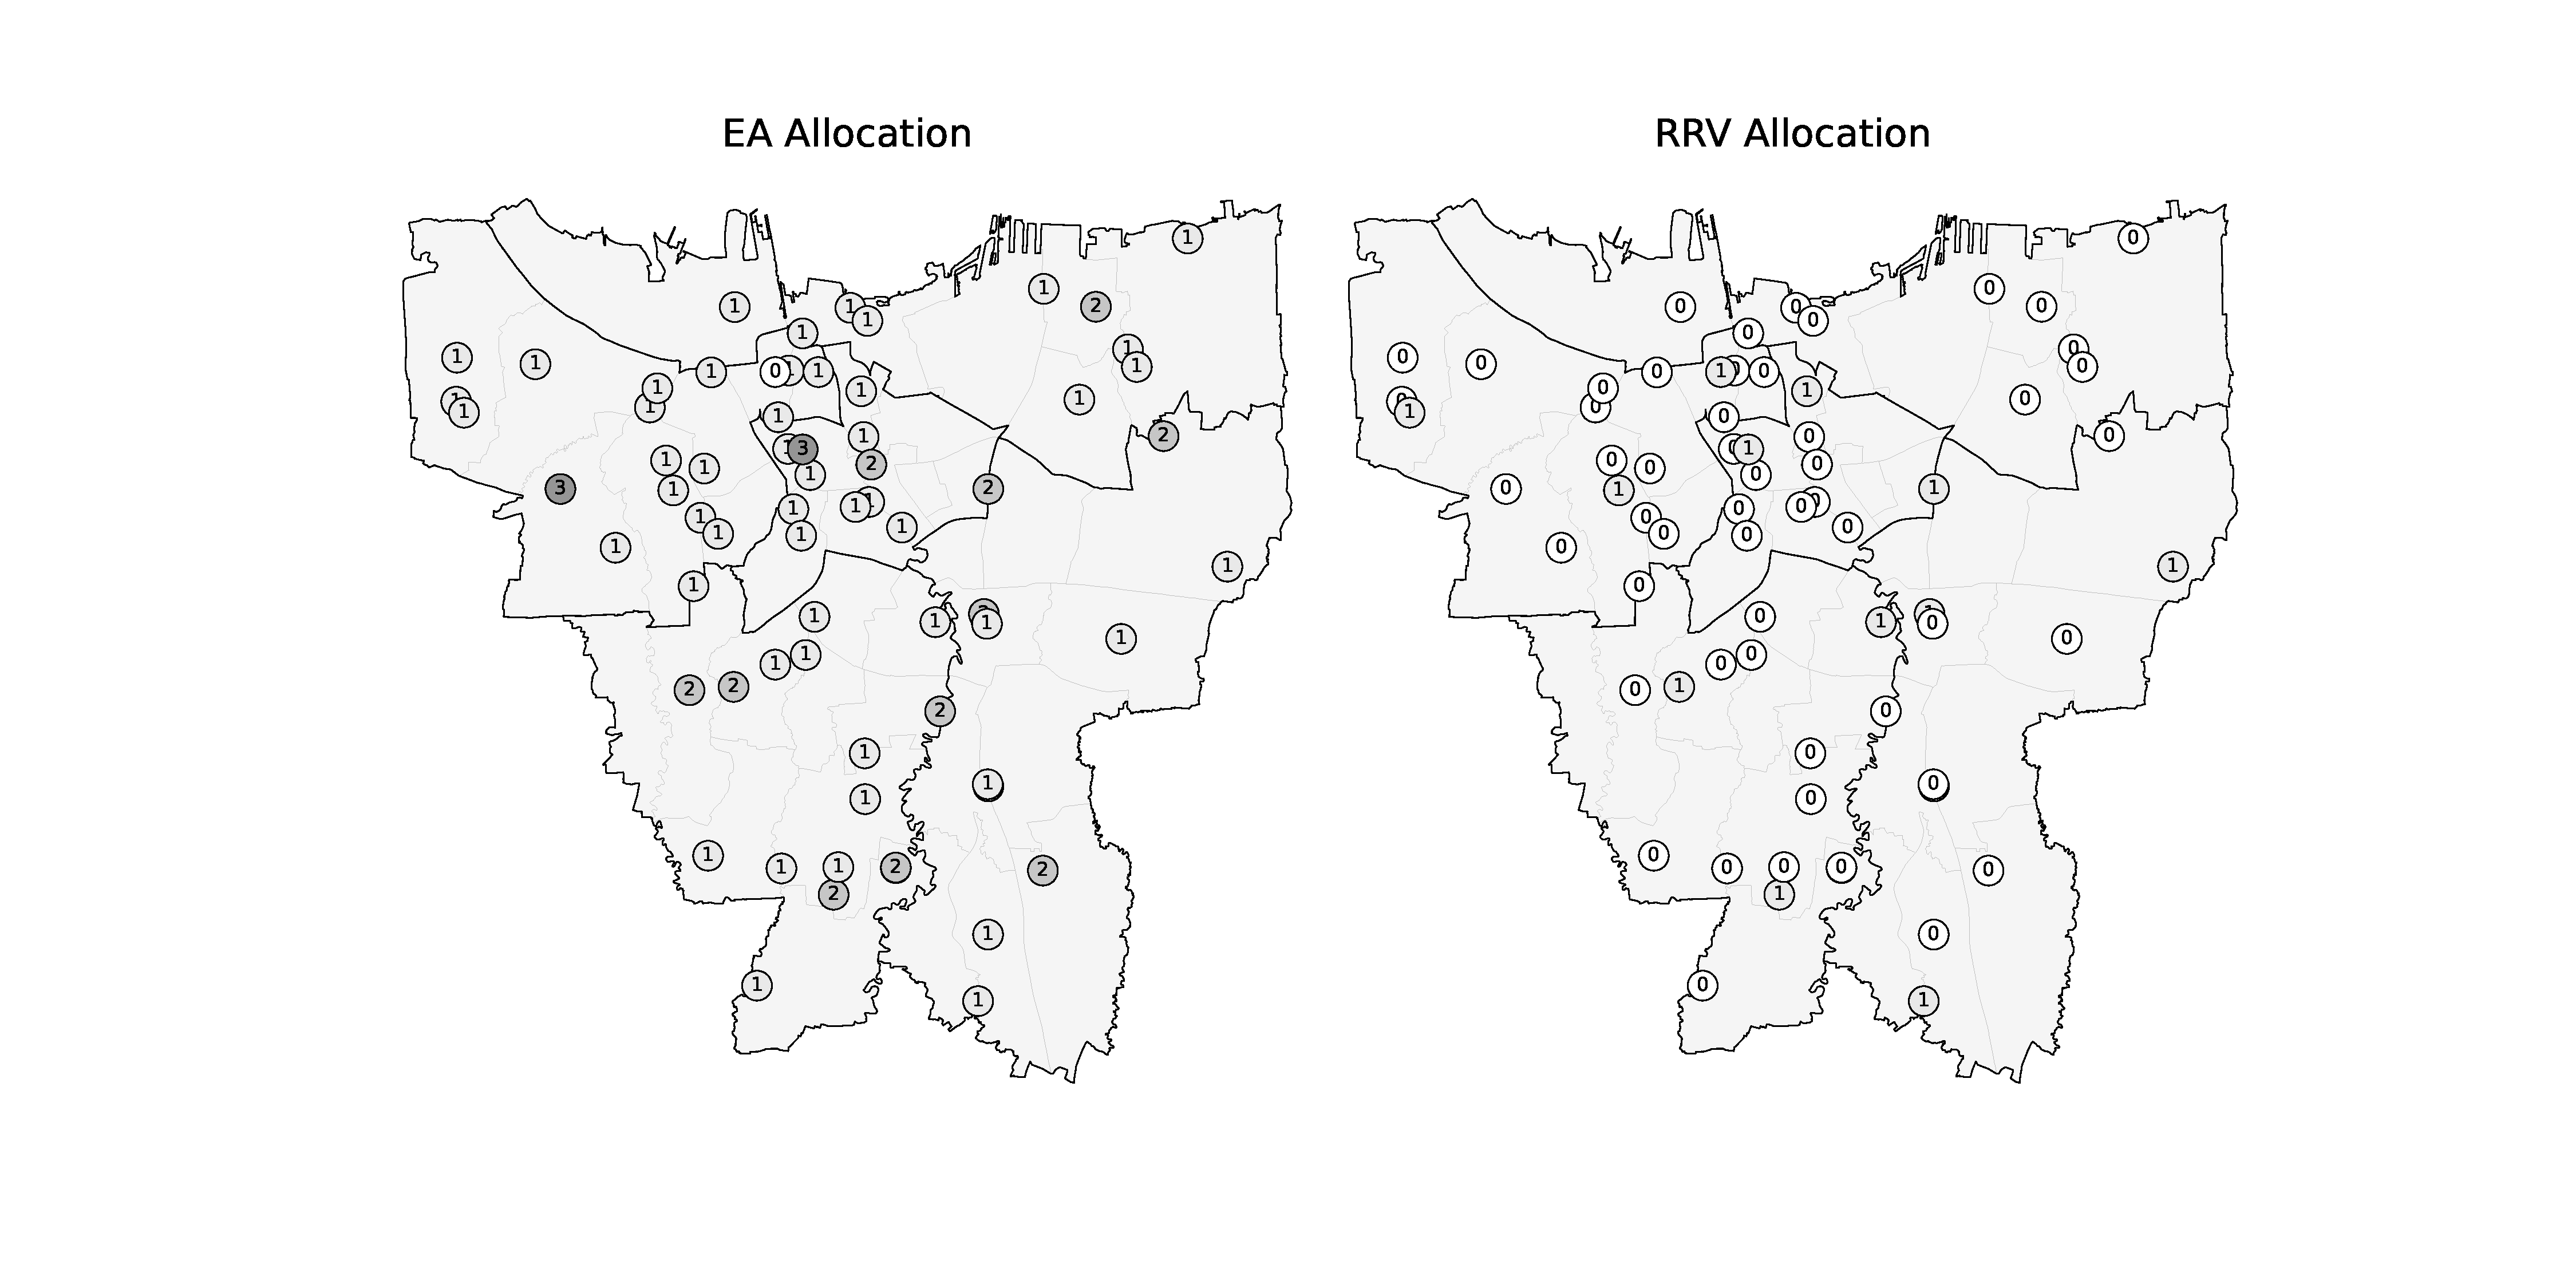
\includegraphics[width=\textwidth]{img/map_current} \caption{Improved allocation
of 81 EAs and 13 RRVs.} \label{fig:optimal_current_allocation} \end{center}
\end{figure}

\begin{table} \begin{center} \begin{tabular}{rrr} \toprule Allocation & Baseline
    & Improved \\ \midrule Ambulance Utilisation & 31.7\% & 31.7\% \\ RRV
    Utilisation & 40.9\% & 40.9\% \\ Mean Response Time (mins) & 16.80 & 16.80
    \\ Overall Survival & 75.5\% & 75.5\% \\ Percent Abandoned & 0.034\% &
    0.034\% \\ \bottomrule \end{tabular} \caption{Comparing KPIs for the current
    and improved allocations.} \label{tbl:current_optimal_compare} \end{center}
    \end{table}


\subsection{Experimental Design}\label{sec:experiment} The heuristic algorithm
described in Section~\ref{sec:cross_entropy} finds allocation of ambulances
across the 67 current ambulance stations for a given resource level, that is for
a given number of EAs and RRVs. We perform experiments to find allocations for
each demand scenario described in Section~\ref{sec:demand_scenarios}, for
resource levels between 60 and 124 EAs, and for two scenarios: a single vehicle
type scenario with no RRVs, and a multiple vehicle type scenario with both EAs
and RRVs. Information supplied by one of the ambulance operators suggested that
in terms of total running costs one EA was approximately equivalent to three
RRVs, and so we consider three RRVs to be one resource.

Run times of the cross-entropy heuristic for allocating all 67 ambulance
stations proved to be impractical. Therefore, working on the assumption that the
best allocations within each municipality were independent of one another, the
heuristic was run on each of the five municipalities (Table~\ref{tbl:jakarta})
independently and the allocations combined. Initially each municipality was
allocated a resource level proportional to their population, and as the
experiments increased the overall resource level, this was added to the
municipality with the worst resource-population ratio, and then the heuristic
was re-ran with it's new resource level.

% In our case study we have 67 ambulance stations, 261 demand locations, we
% considered resource levels between 60 and 100 ambulance equivalents (AE's) in
% various combinations of EA's and RRV's and 4 demand scenarios. 

% Information supplied by one of the ambulance operators suggested that in terms
% of total running costs one EA was approximately equivalent to 3 RRV's. So for
% each resource level between 60 and 100 AE's we considered an equivalent range
% of EA/RRV combinations. In practise we limited this by implementing a rule
% that the number of RRV's could not exceed the number of EA's.

% Experimentation confirmed the assumption that running the optimisation
% algorithm using MESLMHPHF was computationally too expensive when applied to
% the whole problem, so we devised an approach that allowed us to consider each
% municipality (North, South, East, West and Central Jakarta) in turn and then
% combine the results: \begin{enumerate} \item Initially ambulance equivalents
% (AE's) were allocated to each municipality based on demand, with 60 AE's
% available for allocation between the 5 municipalities.  \item Each of the 5
% municipalities was subjected to a series of optimisation runs applying the
% optimisation algorithm to a range of different combinations of EA's and RRV's
% based on their initial AE allocation. Thus for Northern Jakarta the initial
% allocation was 9 AE's and optimisation runs were carried out for 9EA's, 8EA's
% and 3 RRV's, and 7EA's and 6 RRV's. The best result was retained as the
% allocation for that municipality.  \item The results from each municipality
% were then combined to give the optimum initial allocation (for 60 AE's) and a
% combined MESLMHPHF score.  \item The resource level (total AE's) was then
% raised by one, with the additional resource allocated to the municipality with
% the lowest MESLMHPHF score from the previous round, the optimisation runs
% using the different EA/RRV combinations were re-run for this municipality
% only, to get a revised optimal allocation and MESLMHPHF score.  \item The
% result for the chosen municipality was combined with the existing allocations
% from the other 4 municipalities to give the revised optimum allocation, and
% the associated scores for the new resource level.  \item Steps 4 and 5 were
% repeated for each additional resource level until the maximum (100 AE's) was
% reached.  \end{enumerate}



\subsection{Optimisation Results}\label{sec:optimisation_results} Allocations
were found for each resource level between 60 and 124 EA equivalents, for both
single and multiple vehicle scenarios, for each of the four demand scenarios.
Figures~\ref{fig:results_ambulance_utilisation}-\ref{fig:results_overall_survival}
display the obtained KPIs for each of these allocations. It can immediately be
seen that increasing the resource level has a positive effect on all KPIs, with
vehicle utilisations, mean response times, and percentage abandoned decreasing,
and overall survival increasing. Similarly, as expected increasing the demand of
emergency calls has a negative impact on all KPIs.

% \begin{figure} \begin{center} \begin{subfigure}{0.41\textwidth}
% 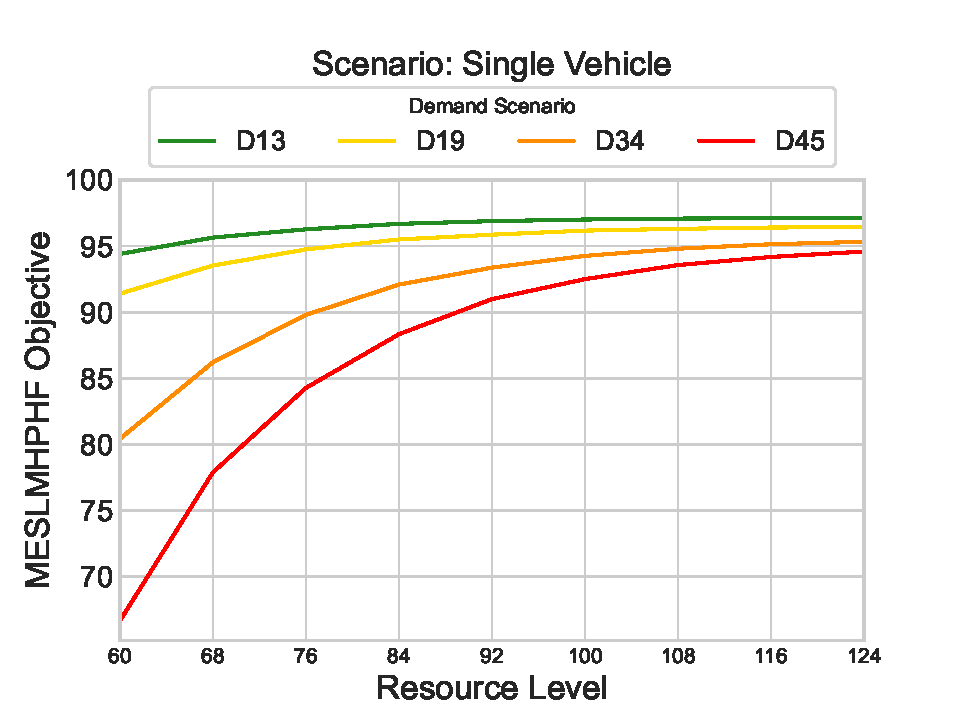
\includegraphics[width=\textwidth]{img/results/single_Objective}
% \caption{Single vehicle type scenario.} \label{fig:results_objective_single}
% \end{subfigure} \begin{subfigure}{0.41\textwidth}
% 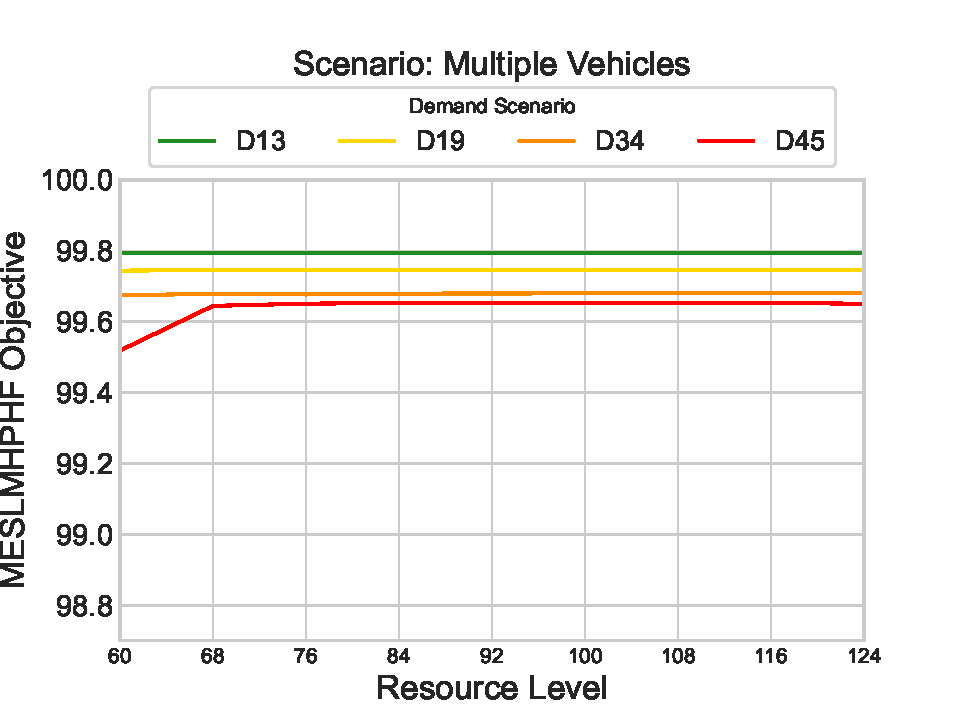
\includegraphics[width=\textwidth]{img/results/multiple_Objective}
% \caption{Multiple vehicle type scenario.}
% \label{fig:results_objective_multiple} \end{subfigure} \end{center}
% \caption{MESLMHPHF score results.} \label{fig:results_objective} \end{figure}

\begin{figure} \begin{center} \begin{subfigure}{0.48\textwidth}
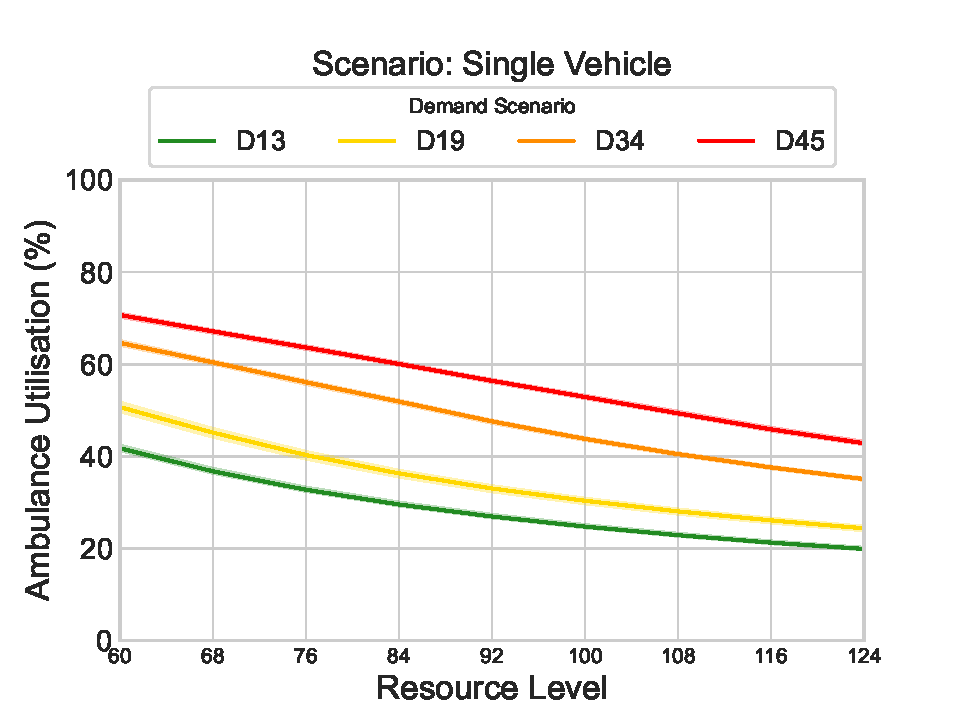
\includegraphics[width=\textwidth]{img/results/single_AmbulanceUtilisation}
\caption{Single vehicle type scenario.}
\label{fig:results_ambulance_utilisation_single} \end{subfigure}
\begin{subfigure}{0.48\textwidth}
    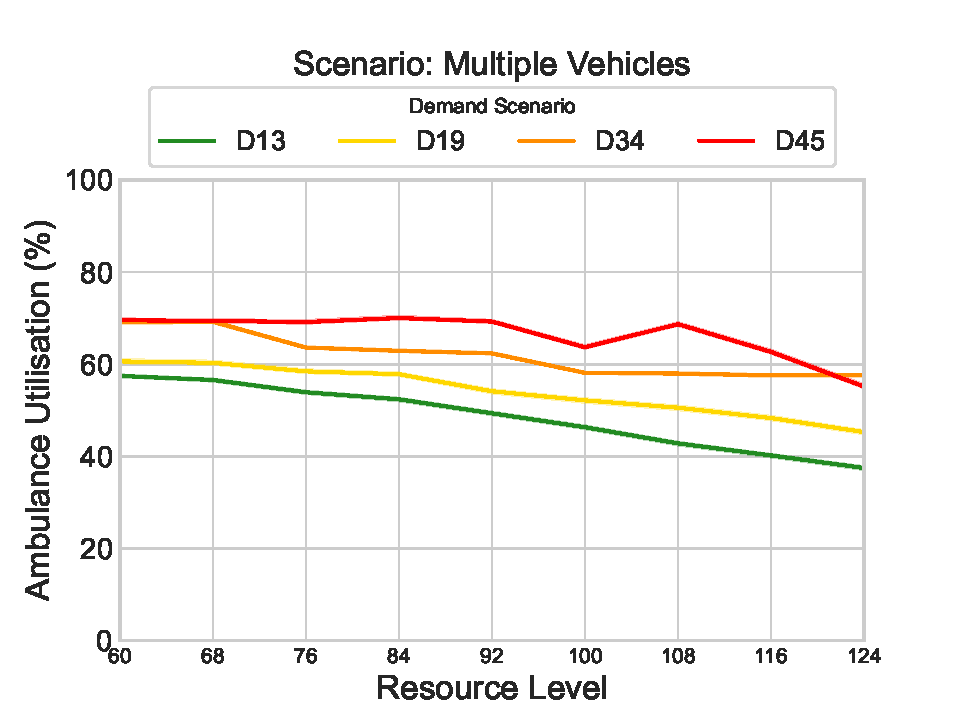
\includegraphics[width=\textwidth]{img/results/multiple_AmbulanceUtilisation}
    \caption{Multiple vehicle type scenario.}
    \label{fig:results_ambulance_utilisation_multiple} \end{subfigure}
    \end{center} \caption{Ambulance utilisation results.}
    \label{fig:results_ambulance_utilisation} \end{figure}

\begin{figure} \begin{center}
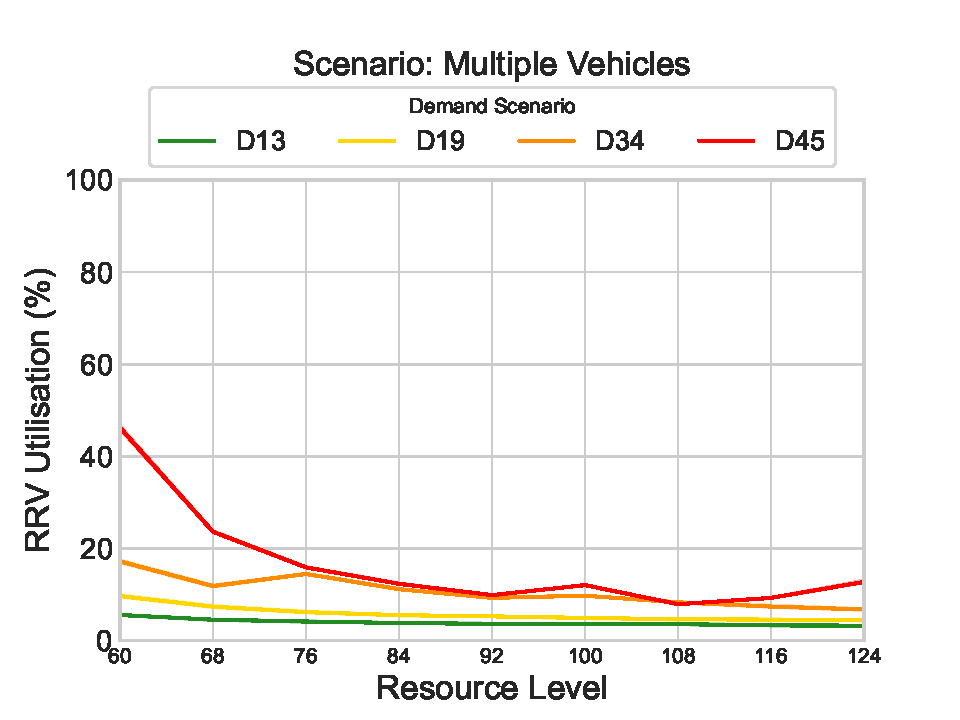
\includegraphics[width=0.48\textwidth]{img/results/multiple_RRVUtilisation}
\end{center} \caption{RRV utilisation results.}
\label{fig:results_rrv_utilisation_multiple} \end{figure}

\begin{figure} \begin{center} \begin{subfigure}{0.48\textwidth}
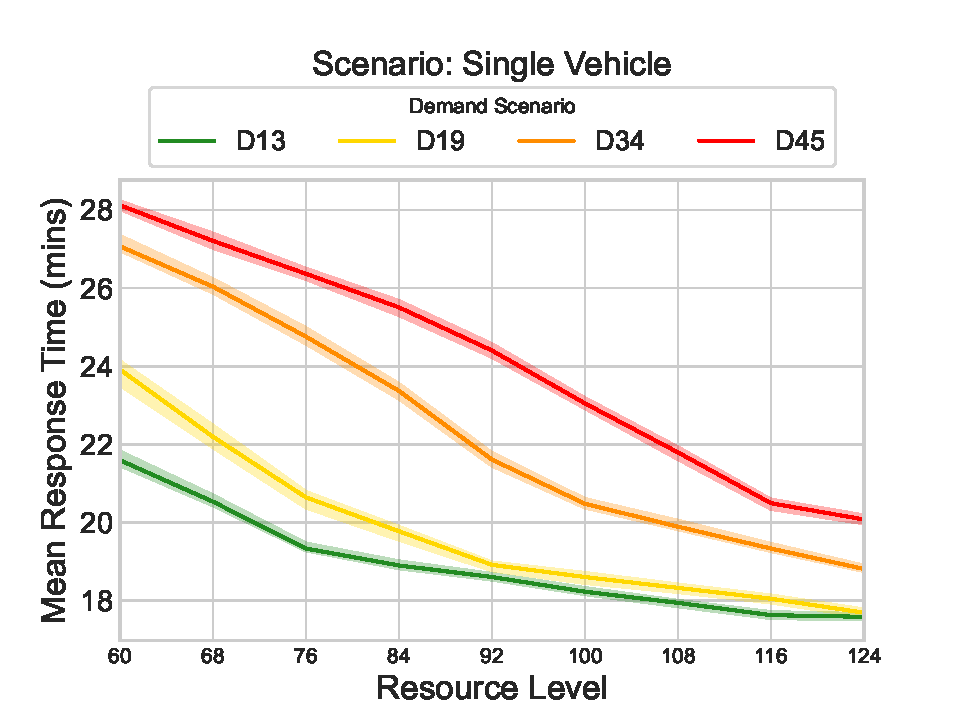
\includegraphics[width=\textwidth]{img/results/single_MeanResponseTime}
\caption{Single vehicle type scenario.} \label{fig:results_response_single}
\end{subfigure} \begin{subfigure}{0.48\textwidth}
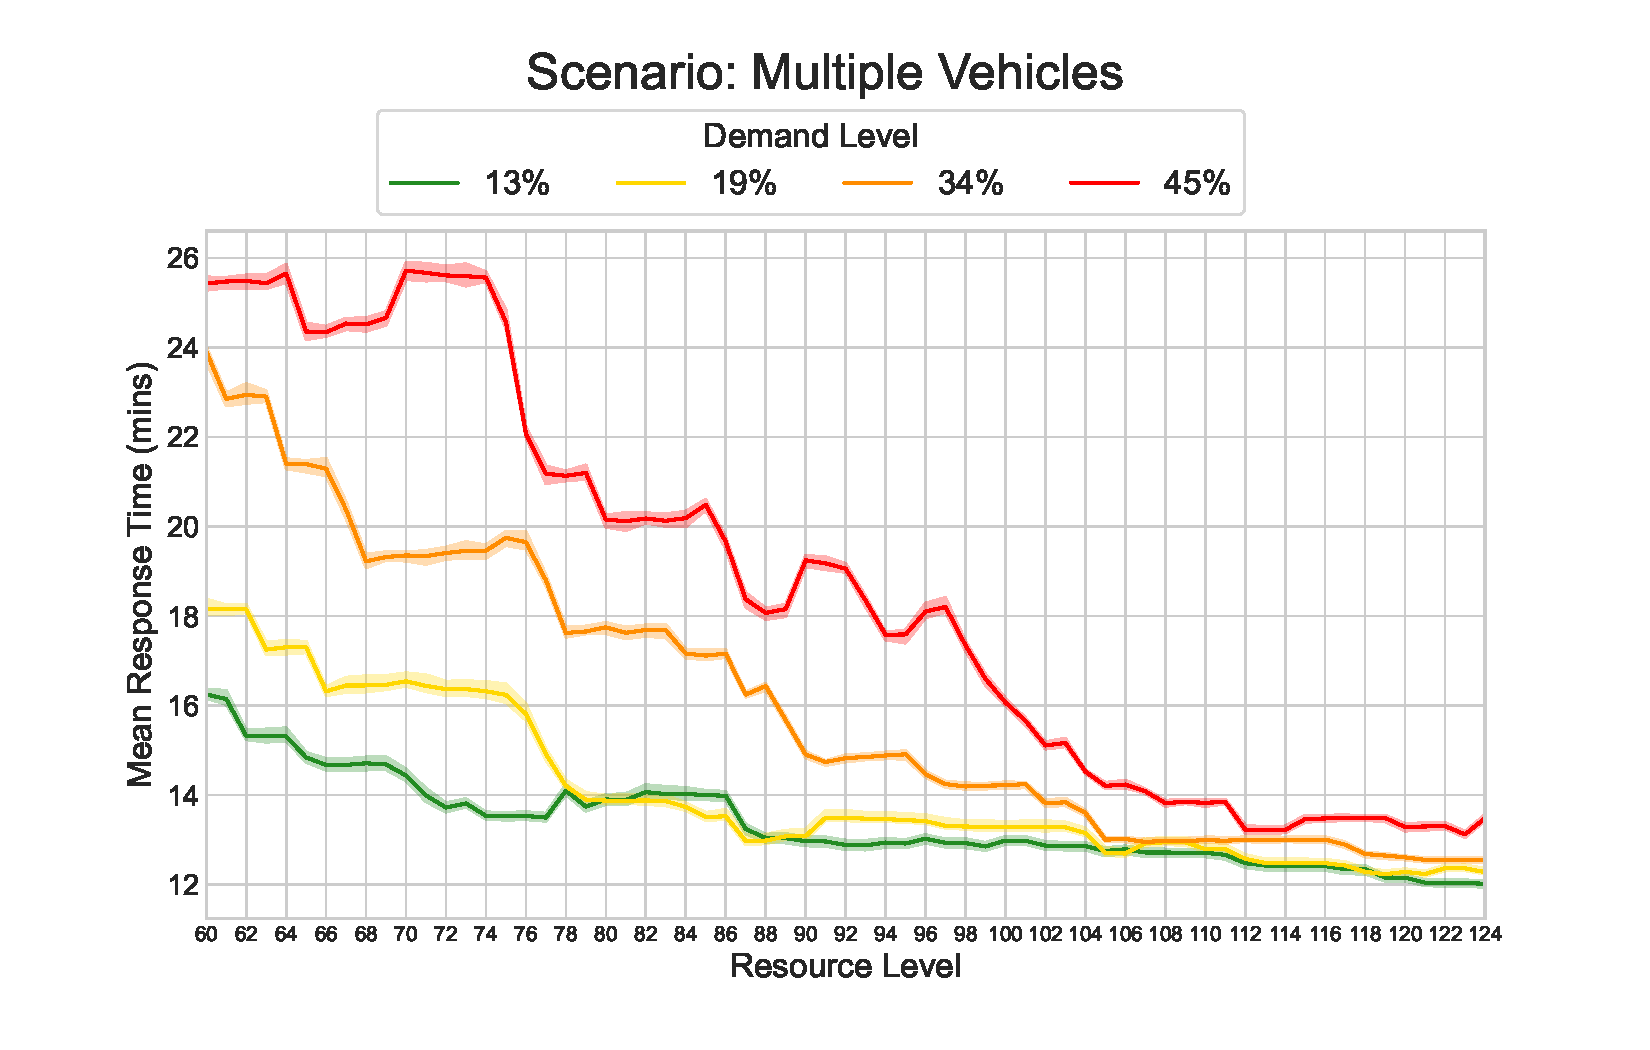
\includegraphics[width=\textwidth]{img/results/multiple_MeanResponseTime}
\caption{Multiple vehicle type scenario.} \label{fig:results_response_multiple}
\end{subfigure} \end{center} \caption{Mean response time results.} \end{figure}

\begin{figure} \begin{center} \begin{subfigure}{0.48\textwidth}
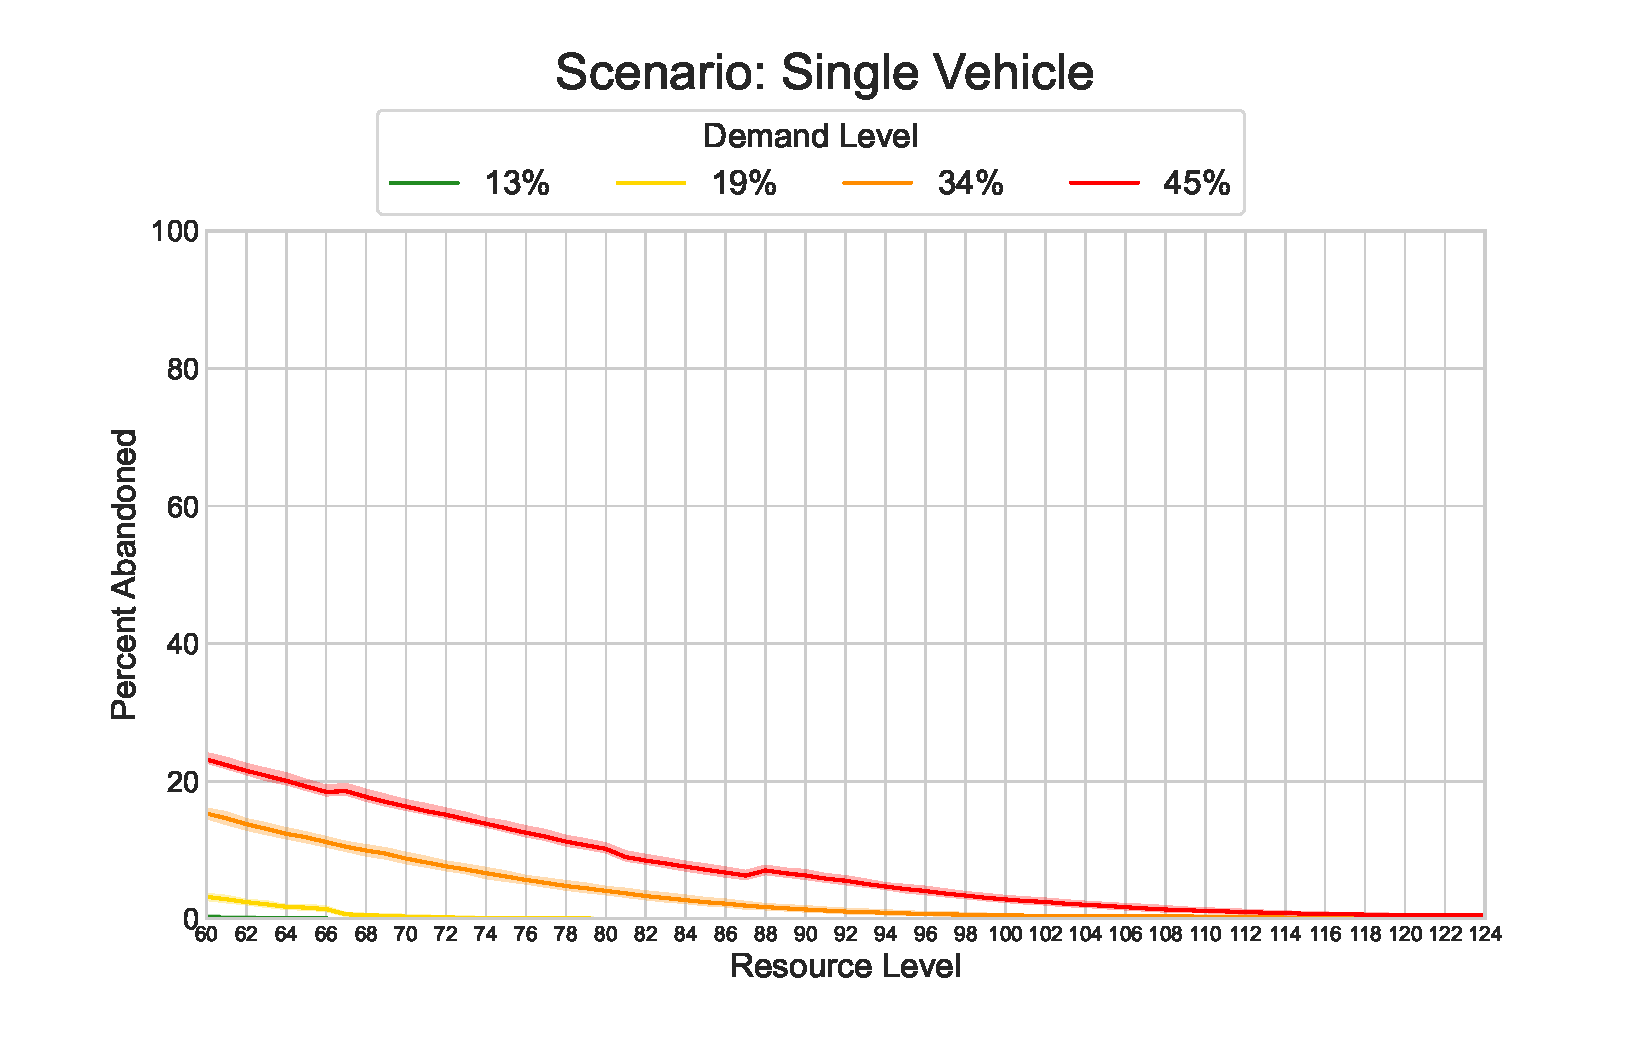
\includegraphics[width=\textwidth]{img/results/single_PercentAbandoned}
\caption{Single vehicle type scenario.} \label{fig:results_abandoned_single}
\end{subfigure} \begin{subfigure}{0.48\textwidth}
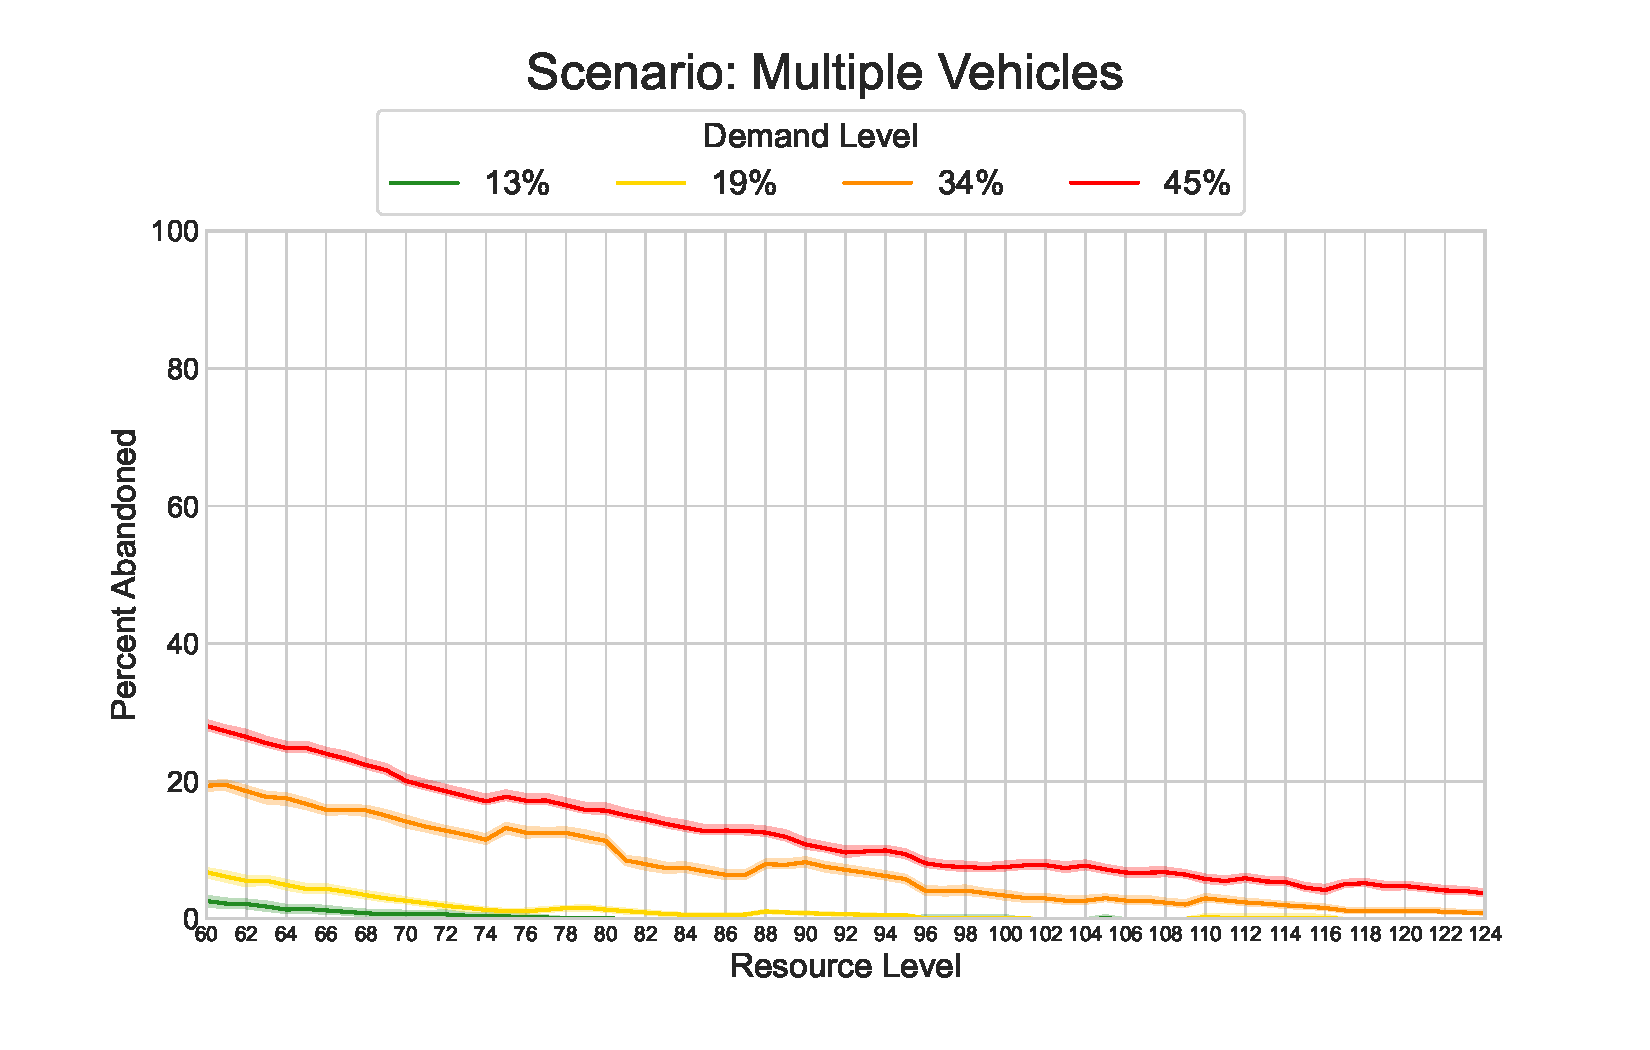
\includegraphics[width=\textwidth]{img/results/multiple_PercentAbandoned}
\caption{Multiple vehicle type scenario.} \label{fig:results_abandoned_multiple}
\end{subfigure} \end{center} \caption{Percent of abandoned calls results.}
\end{figure}

% \begin{figure} \begin{center} \begin{subfigure}{0.48\textwidth}
% 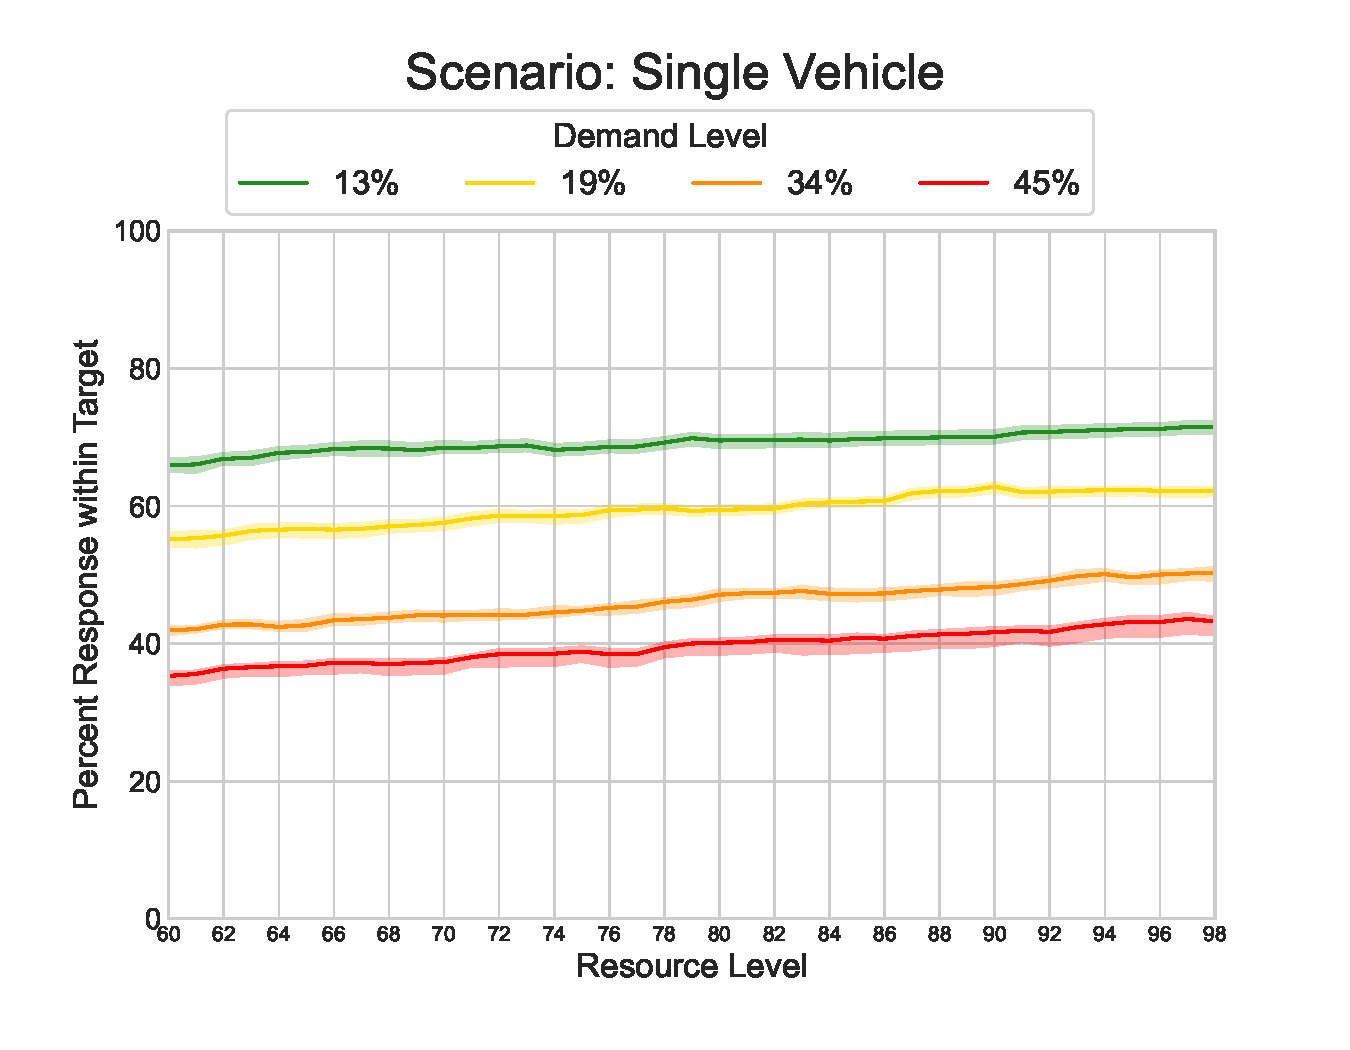
\includegraphics[width=\textwidth]{img/results/single_PercentResponsewithinTarget}
% \caption{Single vehicle type scenario.} \label{fig:results_target_single}
% \end{subfigure} \begin{subfigure}{0.48\textwidth}
% 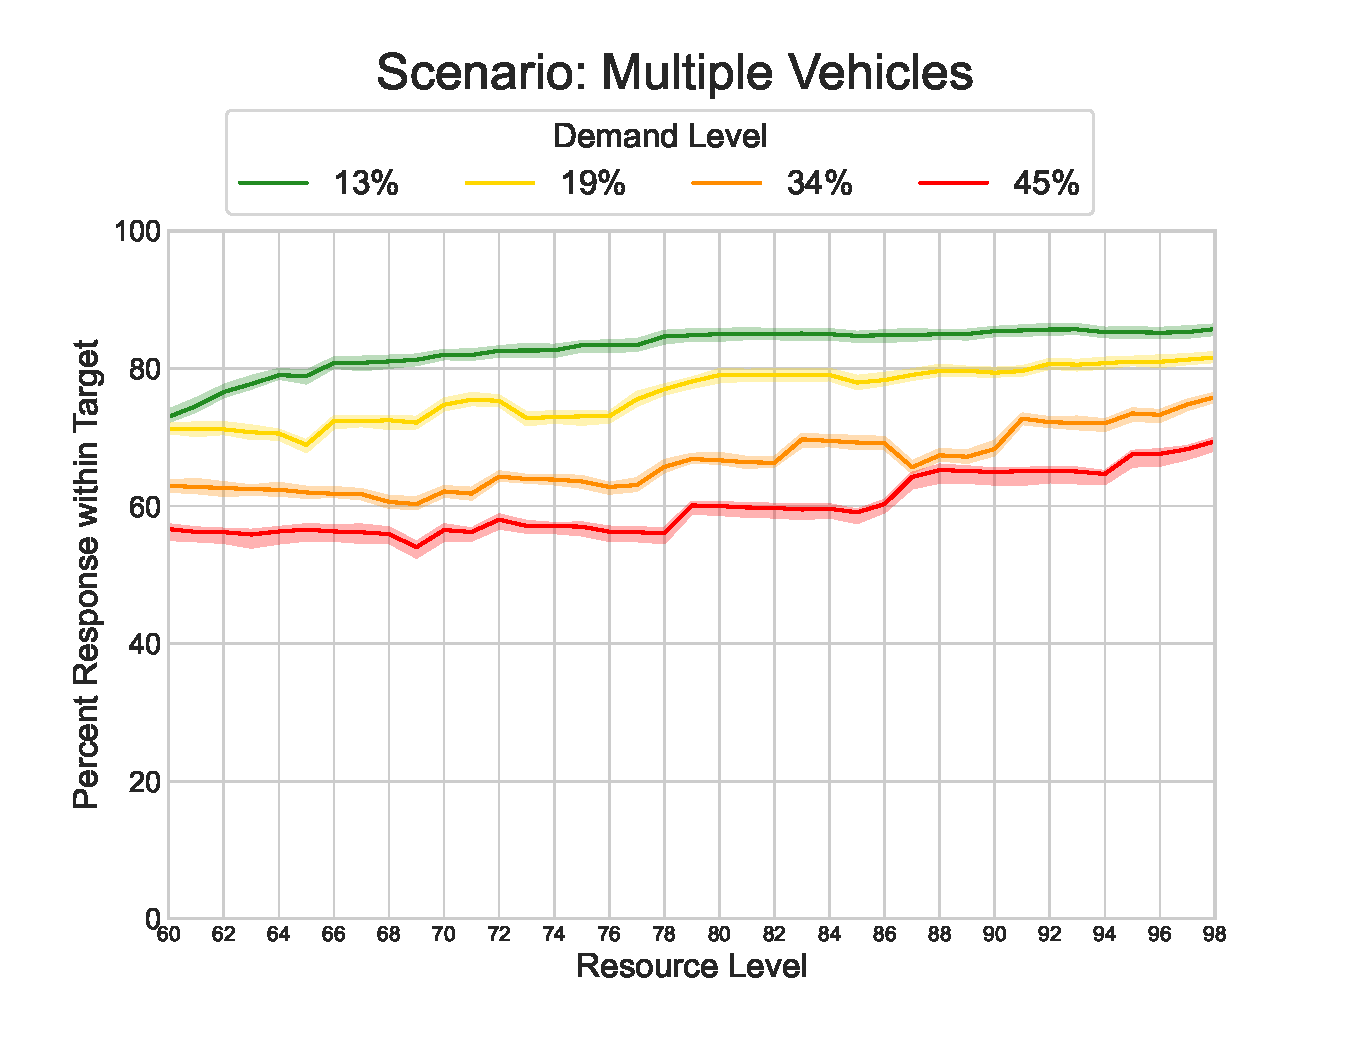
\includegraphics[width=\textwidth]{img/results/multiple_PercentResponsewithinTarget}
% \caption{Multiple vehicle type scenario.} \label{fig:results_target_multiple}
% \end{subfigure} \end{center} \caption{Percent seen within target results.}
% \label{fig:results_within_target} \end{figure}

\begin{figure} \begin{center} \begin{subfigure}{0.48\textwidth}
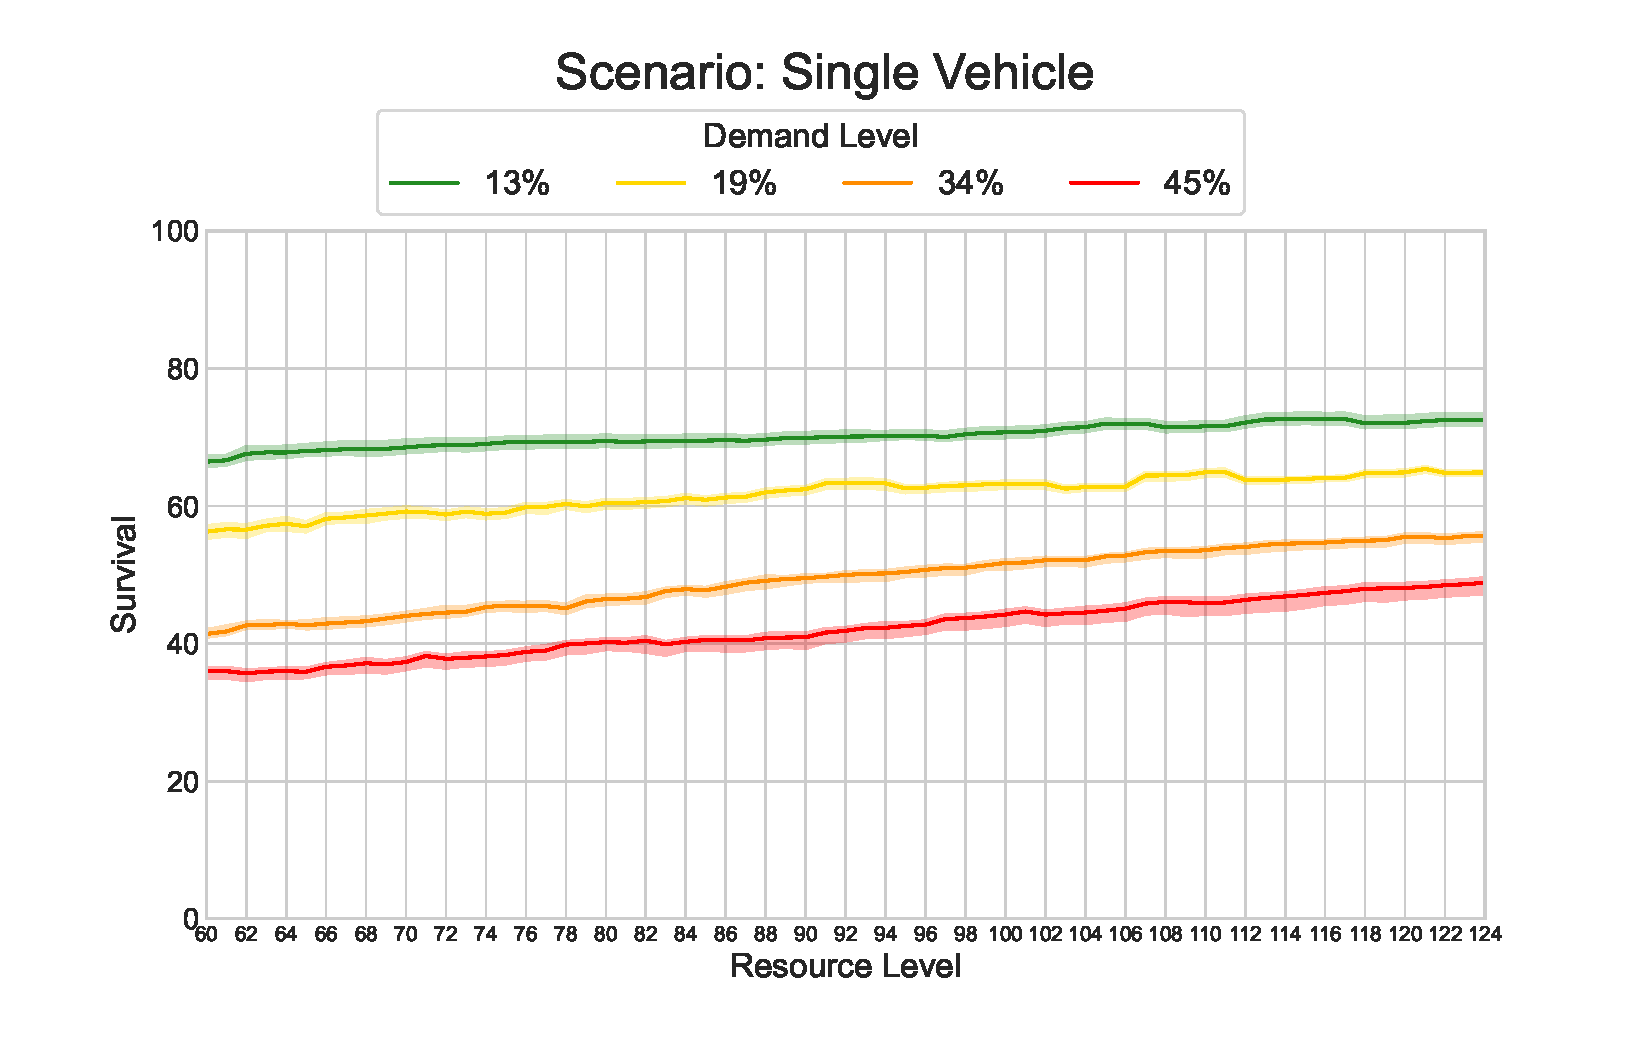
\includegraphics[width=\textwidth]{img/results/single_OverallSurvival}
\caption{Single vehicle type scenario.} \label{fig:results_survival_single}
\end{subfigure} \begin{subfigure}{0.48\textwidth}
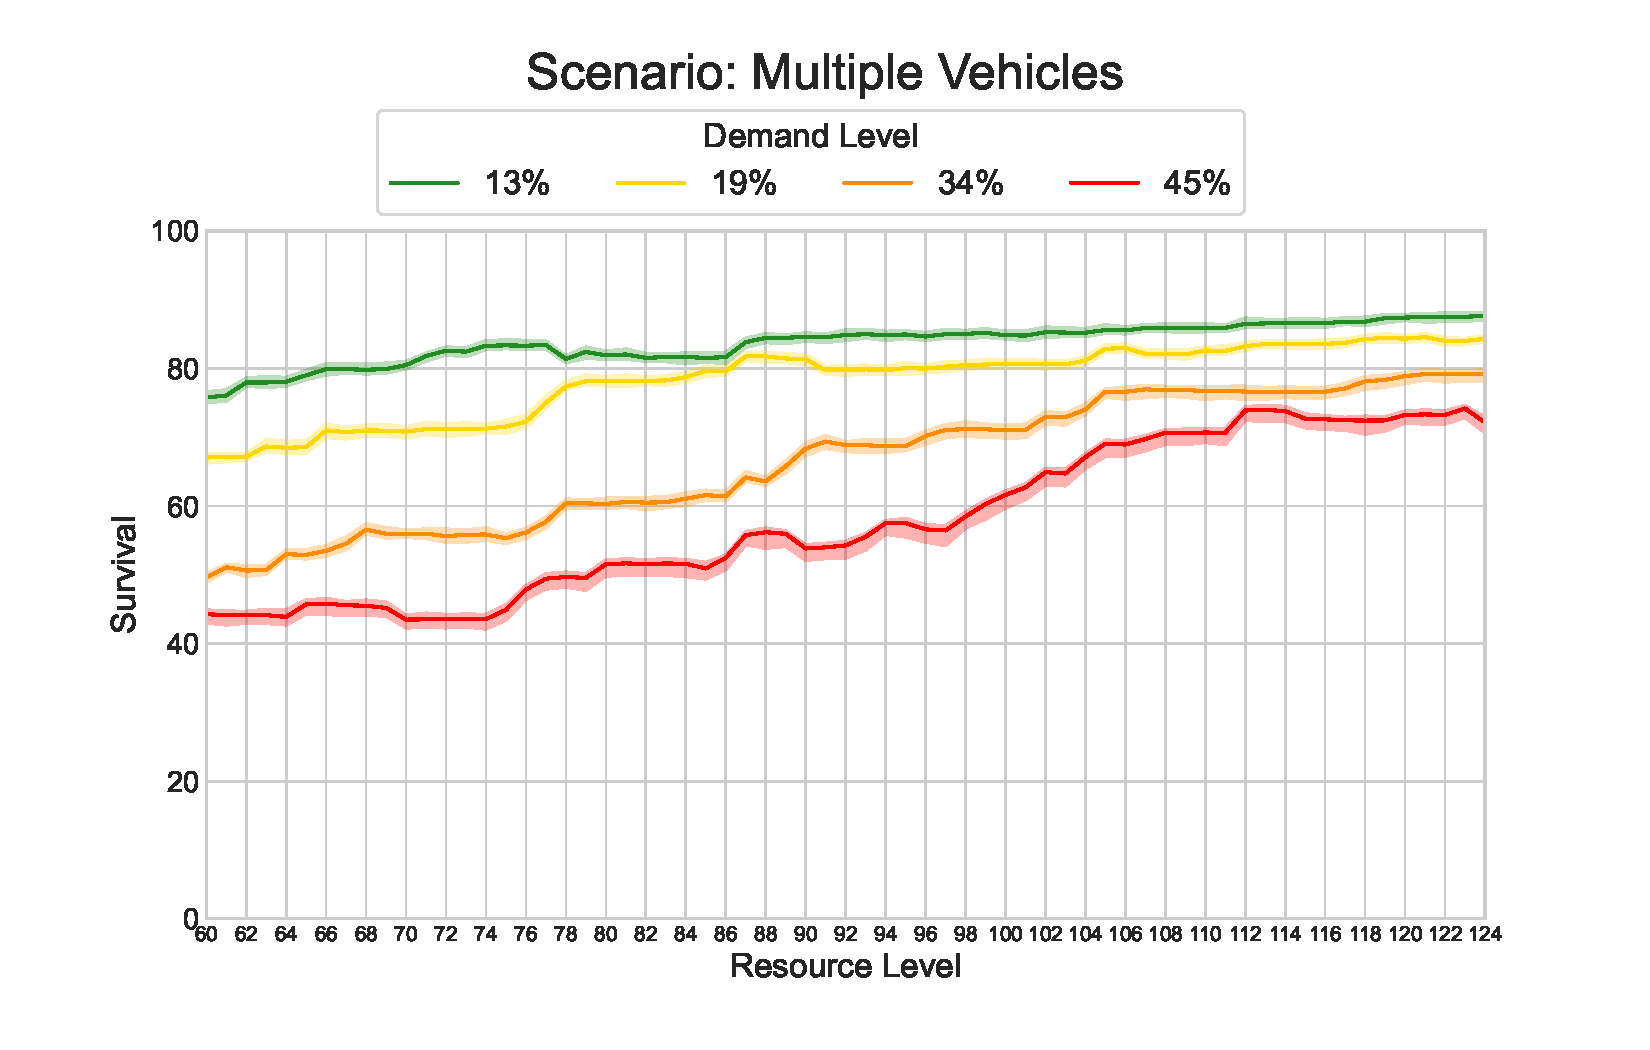
\includegraphics[width=\textwidth]{img/results/multiple_OverallSurvival}
\caption{Multiple vehicle type scenario.} \label{fig:results_survival_multiple}
\end{subfigure} \end{center} \caption{Overall survival results.}
\label{fig:results_overall_survival} \end{figure}

It is particularly interesting to compare the scenario in which single vehicle
types (only emergency ambulances) were allocated against the scenario where
multiple vehicle types (both emergency ambulances and rapid response vehicles)
were allocated. For equivalent resource levels, introducing secondary vehicles
increases ambulance utilisation, and so decreases availability, resulting in an
increase in abandoned calls. However, introducing secondary vehicles also
results in a large decrease in the mean response times, and so a large increase
in the percentage of patients seen within target.

It is also noticeable that the increases or decreases in the simulation derived
KPIs are not necessarily monotonic with increases in resource level. This is due
to the derived allocations being based on the MESLMHPHF score only, which is a
measure of survival, while the simulation derived KPIs are indirect measures of
performance. This may indicate that these indirect measures of performance, such
as mean response times or percentage within target, are not good indicators of
survival.

Crucially, the plots show that the allocations produced by the optimisation
algorithm perform better than the current allocation for the same demand and
resource levels. The current levels include 81 EAs and 13 RRVs, so a resource
level of 85.33, with multiple vehicles. Comparing the derived allocations for
this level in
Figures~\ref{fig:results_ambulance_utilisation}-\ref{fig:results_overall_survival}
to the results given in Table~\ref{tbl:current_grid_results}, the derived
allocations give lower ambulance and RRV utilisations, lower mean response
times, and a higher percentage of patients seen within target.

As experiments were run across all demand scenarios, we can see how much more
resources would be required, if optimally located, to achieve a similar level of
service as is currently offered, when demand increases.
Table~\ref{tbl:equivalent} shows, for each demand scenario, the minimum resource
level and vehicle type breakdown required to meet the current level in each of
the following KPIs: mean response time, overall survival, and percentage of
calls abandoned. For example, in order to maintain the current 75.48\% overall
survival, under the demand\_19 scenario the city would require 63 EAs and 45
RRVs.  It is noticeable that fewer resources are required to maintain the
current mean response time than to maintain the current overall survival.

\begin{table} \begin{center} \resizebox{\textwidth}{!}{% \begin{tabular}{cccc}
        \toprule Demand Scenario & Mean Response Time & Overall Survival &
        Percent Abandoned \\ \midrule \textbf{demand\_13} & 60, (50, 30) & 60,
        (50, 30) & 80, (66, 42) \\ \textbf{demand\_19} & 70, (60, 30) & 78, (63,
        45) & 101, (79, 66) \\ \textbf{demand\_34} & 88, (75, 39) & 106, (83,
        69) & $>$ 124 \\ \textbf{demand\_45} & 99, (85, 42) & $>$ 124 & $>$ 124
        \\ \midrule Current Level & 16.8 mins & 75.48\% & 0.0339\% \\
\bottomrule \end{tabular}% } \caption{Resources required to maintain current KPI
levels when optimising locations under the four demand scenarios.}
\label{tbl:equivalent} \end{center} \end{table}

\section{Discussion \& Conclusions}\label{sec:discussion} This paper describes
the development of EMS demand and capacity models and their application to the
city of Jakarta, Indonesia. To our knowledge, this is the first such study of
analysing emergency ambulance services in Jakarta, and the work has directly
assisted and guided providers and the government to make investment decisions
for a coordinated and free to use EMS.

Firstly, a discrete event simulation model has been used to evaluate existing
and potential heterogeneous vehicle ambulance feet allocations in terms of key
performance measures, such as response times, response time targets, and vehicle
utilisation rates. This takes into consideration geospatial demand and travel,
and temporal variation in demand and traffic levels. A novel feature of our
approach is that the model comprises of sequential simulations, feeding data
directly from one into the other in order to simulate primary and secondary
vehicles separately while maintaining synchronicity, with the overall aim of
reducing the complexity of the simulation logic.

Secondly, we have considered patient survival and outcomes within a developed
cross-entropy heuristic. By considering geospatial travel times and accounting
for the varying needs of different patient types though categorising patients by
priority and through using different survival function profiles, an expected
overall survival was given. This could be used within a optimisation processes,
in this case a cross-entropy heuristic, to find vehicle fleet allocations that
maximise expected survival. This expected survival function extends previous
work in \cite{Knight2012918} to include more than one vehicle type.

Both models investigate ambulance service activity in the case of heterogeneous
patients and heterogeneous fleets. Heterogeneous patient groups consider those
with distinct demand profiles, priorities, and survival functions. Heterogeneous
fleets concern different types of vehciles, in our case emergency ambulances
(EAs) which respond to every patient, and Rapid Response Vehicles (RRVs) which
can be utilised to reach patients faster, despite being unable to transport
patients themselves.

Using a combination of models has permitted an approach that can capture
performance measures or take into account factors that each model in isolation
can not. For example, the maximum expected survival model is a lot more
appropriate for use within an optimisation process as the runtimes are a far
more reasonable than the simulation. On the other hand, the simulation allows
for greater complexity such as temporal demand, and is able to capture a greater
range of KPIs.

A key feature of both models, and their novelty, is the consideration of
heterogeneous fleets. In a highly populated area such as Jakarta (around 16,000
population per km$^2$), the inclusion of RRVs such as paramedics on motorbikes
is very important, given RRVs can access areas that cannot easily or quickly be
accessed by ambulances. Results from both the optimisation and simulation
research showed that the RRVs can help increase the overall survival and reduce
the response times, especially crucial when responding to life threatening
events such as cardiac arrests \cite{holmen2020shortening}. 

The results of our research also suggest that allocation strategies may not be
intuitive to ambulance service managers, further emphasising the value of a
modelling approach. For example, senior managers suggested the use of a grid
allocation to maximise geographic coverage, with ambulances equally spread
across the city. This was shown to be sub-optimal because neighbourhoods have
different population densities and characteristics. For example, the number of
daily commuters in Jakarta is considerably high during day time due to work and
education \cite{BPS_Jakarta_migrasi}. Municipalities where trading, educational
institutions, and offices are concentrated may become more populated during day
time. The model has quantified the deterioration in response times and patient
outcomes should a fixed grid system be implemented, leading to 119 to drop this
consideration.

The ambulance posts in Jakarta depend on the service provider. Those ambulances
provided by the government are in various locations including government
buildings as well as community clinics and sub-district hospitals. In our case,
we used current ambulance posts as the locations for allocating the resources.
As demands for ambulances may change from time to time, future work could
evaluate different (and perhaps dynamic) ambulance posts that depend on changing
demand volumes in neighbourhoods by time of the day.

The data used for ambulance demand covered one year from 1 January to 31
December 2019, prior the COVID-19 pandemic. Recent studies related to ambulance
demand indicate that the  pandemic has severely impacted on the utilisation of
EMS, for examples in call volumes \cite{csan2021effects} and in specific medical
conditions such as trauma \cite{ azbel2021effects}, and possibly still continue
to affect demand. Ambulance providers, such as 118 and 119, may use our
modelling tools to incorporate future demand data and re-evaluate resource
needs. To aid this, we are currently working on interfacing the simulation and
optimisation into a single easy to use decision support tool with a dashboard
(data visualiser). 

Studies have shown that the quality in pre-hospital data collection varies
considerably in Indonesia \cite{hooper2019_datacollection}. We encountered
similar challenges and have suggested to 119 and the Indonesian Government that
they should continue to strive to improve the coverage and quality of data
collection. Future work could explore in more depth unmet demand that is not
recorded in the ED or in the ambulance data.

Indonesia is a vast country with an uneven population density and varying
quality of available healthcare resources. The models have been parameterised
with data from a high population, high density urban area which is also
relatively well resourced with healthcare facilities compared to other regions
in the country. Ambulance services in rural areas of Indonesia may not have the
same quality in management and organisation compared to the capital, Jakarta. We
intend to conduct future studies to apply the developed models to analyse
ambulance demand and allocations in different areas of Indonesia, including in
rural regions.

In conclusion, the developed models have demonstrated a novel approach in
modelling ambulance allocations that incorporate multiple vehicle types and
health conditions, whilst also capturing patient survival. Our work has already
informed major decisions on the design of a free to use and coordinated EMS
system for Jakarta. Ongoing collaboration will continue to assist ambulance
providers and the Indonesian Government in providing evidence-based decision
making for the benefit of patients and the population they serve, including the
exploration of the roll-out of 119 beyond Jakarta to other regions of Indonesia. 

\section*{CRediT authorship contribution statement}

From Computers and OR, select from:\\

Conceptualisation; Funding acquisition; Investigation; Methodology; Project
administration; Resources; Software; Supervision; Validation; Writing - original
draft; Writing - review \& editing.\\


{\bf Geraint Palmer:} Conceptualisation, Investigation, Methodology, Software,
Writing – original draft\\

{\bf Sarie Brice:} Conceptualisation, Investigation, Methodology, Writing –
original draft\\

{\bf Daniel Gartner:} Conceptualisation, Funding acquisition, Methodology,
review \& editing.\\

{\bf Paul Harper:} Conceptualisation, Investigation, Methodology, Funding
acquisition, Resources, Project administration, Writing – review \& editing.\\

{\bf Vince Knight:} Conceptualisation, Funding acquisition, Methodology,
Software, review \& editing.\\

{\bf Leanne Smith:} Methodology.\\

{\bf Mark Tuson:} Conceptualisation, Investigation, Methodology, Software,
Writing – original draft\\



\section*{Acknowledgements} The study was funded by EPSRC with grant no:
EP/T003197/1. We would like to express our sincere gratitude to Indonesian
emergency ambulance providers including 118 and 119 for their support, insights
and provision of data. In particular we wish to thank Professor Aryono Djuned
Pusponegoro and Ms Asti Puspita Rini, Founder and Director of 118 Ambulance
Service Foundation and Dr Winarto, Head of the 119 Ambulance Service in Jakarta.

% \section*{Supplementary material} Simulation model documentation, based on
% Strengthening the reporting of empirical simulation studies (STRESS)
% guidelines \cite{Monks2019} is provided.


\appendix

\section{Annotated Objective Function}\label{apx:annotated}
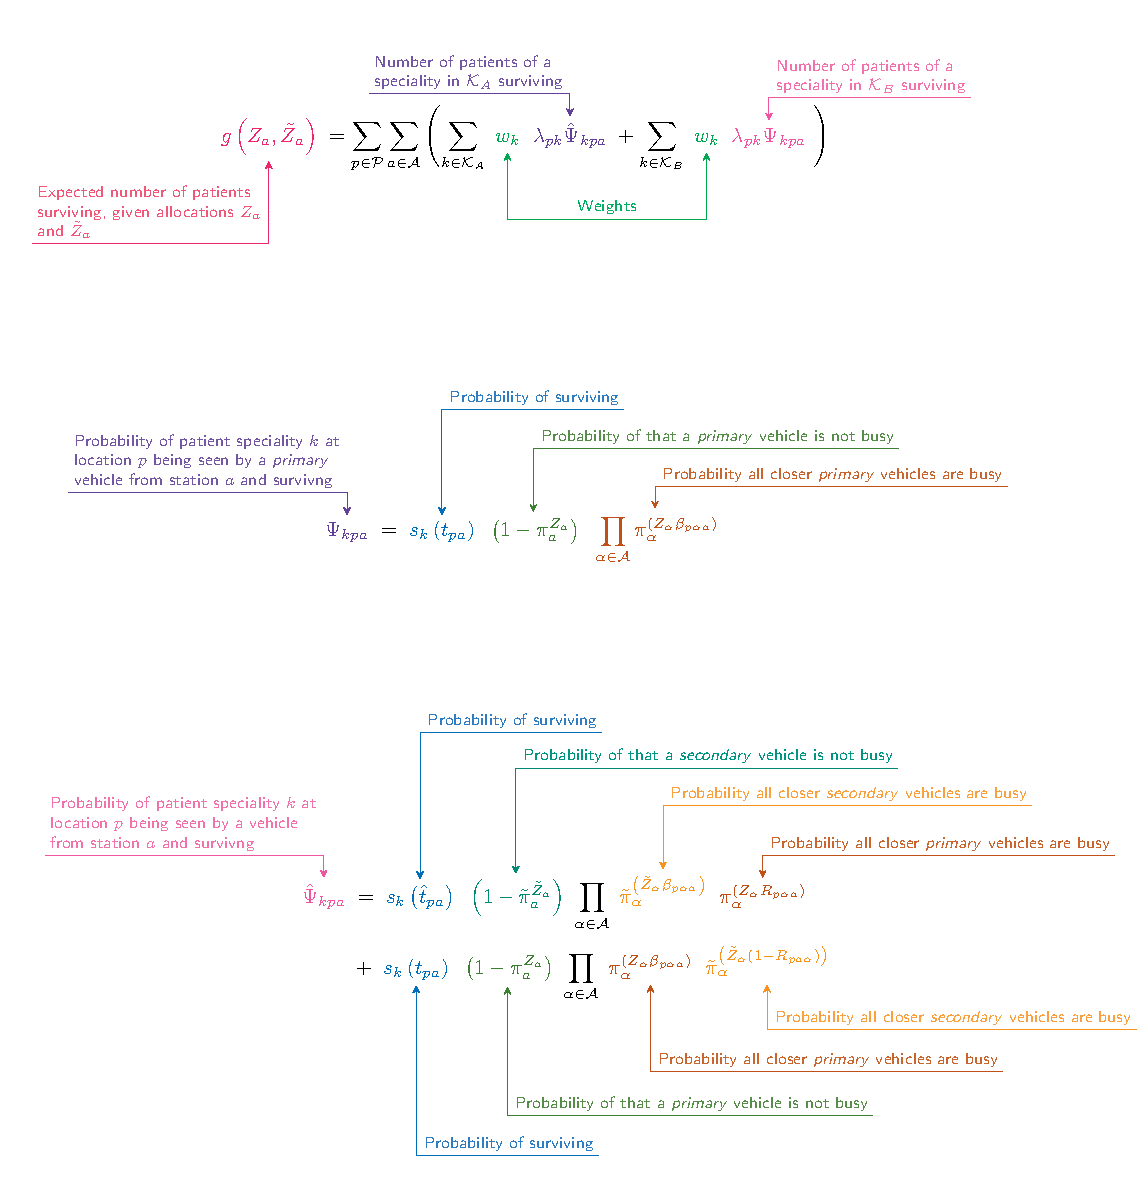
\includegraphics[width=\textwidth]{img/annotate}

\section{Model Parameters} \label{apx:parameters} Call arrival rates
$\lambda_{pk}$ are derived from 2019 demand data slit by municipality and
speciality, and time of day. Probabilities $q_{pky}$ are similarly derived from
the 2019 data of transit journeys. All traffic-free travel times are found using
Google Maps API, while time-dependent traffic delays are found from the TomTom
website. The other models are parameterised in the following way:
\begin{itemize} \item From a sample of calls the time at site $G_k$ was found to
            follow a lognormal distribution with parameters $\mu = -0.6219$ and
            $\sigma = 0.8048$. For the case of Jakarta this was modelled
            identically for all specialities $k$. Comparison between the
            lognormal fit and the sampled times are given in
            Figure~\ref{fig:lognorm_fit}.  \item From discussions with staff at
                the ambulance service in Jakarta, the time at hospital $J_k$ was
                modelled as a Uniform distribution between 40 and 60 minutes for
                the emergency specialities A1 and A2, and between 20 and 30
                minutes for non-emergency speciality B.  \item From discussions
with staff at the ambulance service in Jakarta, the refill time $\Theta$ is
taken to be 60 minutes for an emergency ambulance, and 15 minutes for an RRV.
\end{itemize}

\begin{figure}[ht] \centering
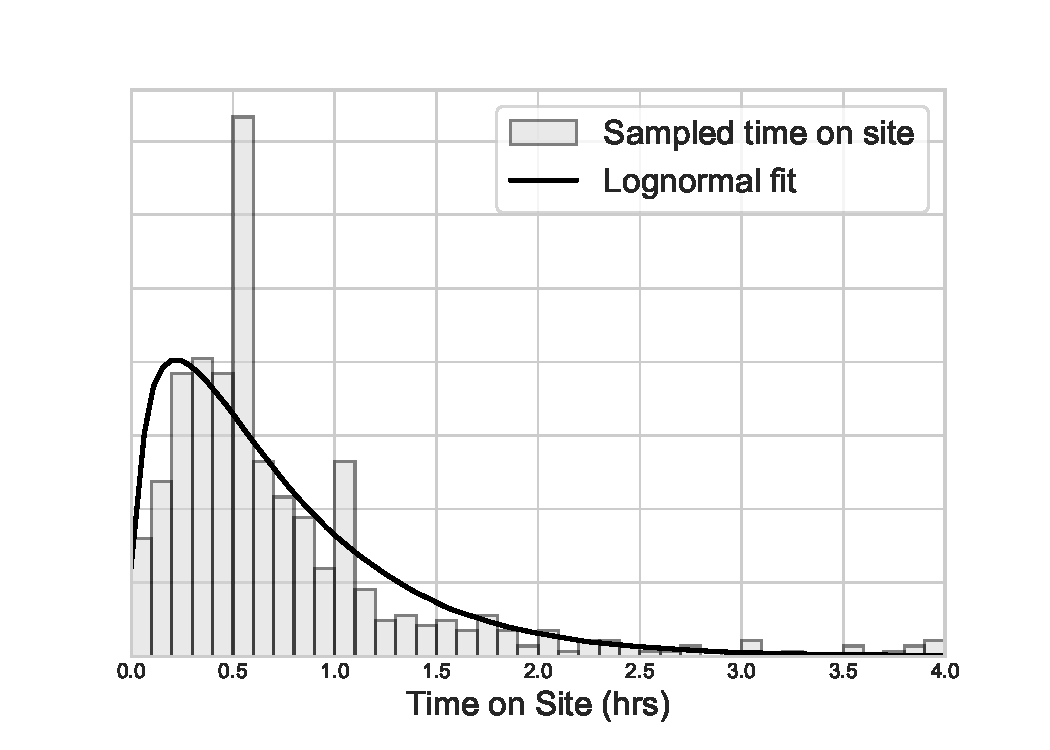
\includegraphics[width=0.6\textwidth]{img/time_on_site_fit.pdf}
\caption{Comparison between the sampled time on site and the lognormal fit.}
\label{fig:lognorm_fit} \end{figure}

% \footnotesize

\bibliographystyle{plainnat}

% AUTHOR: Include your bib file here
\bibliography{literature}

%\section*{AUTHOR BIOGRAPHIES}



\end{document}
